% kaobook
% LaTeX Template
% Version 1.2 (4/1/2020)
%
% This template originates from:
% https://www.LaTeXTemplates.com
%
% For the latest template development version and to make contributions:
% https://github.com/fmarotta/kaobook
%
% Authors:
% Federico Marotta (federicomarotta@mail.com)
% Based on the doctoral thesis of Ken Arroyo Ohori (https://3d.bk.tudelft.nl/ken/en)
% and on the Tufte-LaTeX class.
% Modified for LaTeX Templates by Vel (vel@latextemplates.com)
%
% License:
% CC0 1.0 Universal (see included MANIFEST.md file)
%
%%%%%%%%%%%%%%%%%%%%%%%%%%%%%%%%%%%%%%%%%

%----------------------------------------------------------------------------------------
%	PACKAGES AND OTHER DOCUMENT CONFIGURATIONS
%----------------------------------------------------------------------------------------

\documentclass[
	fontsize=10pt, % Base font size
	twoside=false, % Use different layouts for even and odd pages (in particular, if twoside=true, the margin column will be always on the outside)
	%open=any, % If twoside=true, uncomment this to force new chapters to start on any page, not only on right (odd) pages
	%chapterprefix=true, % Uncomment to use the word "Chapter" before chapter numbers everywhere they appear
	%chapterentrydots=true, % Uncomment to output dots from the chapter name to the page number in the table of contents
	numbers=noenddot, % Comment to output dots after chapter numbers; the most common values for this option are: enddot, noenddot and auto (see the KOMAScript documentation for an in-depth explanation)
	%draft=true, % If uncommented, rulers will be added in the header and footer
	%overfullrule=true, % If uncommented, overly long lines will be marked by a black box; useful for correcting spacing problems
]{kaobook}

% Set the language
\usepackage[english]{babel} % Load characters and hyphenation
\usepackage[english=british]{csquotes} % English quotes

% frontpage 
\usepackage{ae,aecompl}
\usepackage{eso-pic}
\usepackage{array}

% Load packages for testing
\usepackage{blindtext}
\usepackage{lscape}
%\usepackage{showframe} % Uncomment to show boxes around the text area, margin, header and footer
%\usepackage{showlabels} % Uncomment to output the content of \label commands to the document where they are used

% Load the bibliography package
\usepackage{styles/kaobiblio}
\addbibresource{main.bib} % Bibliography file

% Load mathematical packages for theorems and related environments. NOTE: choose only one between 'mdftheorems' and 'plaintheorems'.
\usepackage{styles/mdftheorems}

%\usepackage{styles/plaintheorems}

\graphicspath{{examples/documentation/images/}{images/}} % Paths in which to look for images

\makeindex[columns=3, title=Alphabetical Index, intoc] % Make LaTeX produce the files required to compile the index

%\makeglossaries % Make LaTeX produce the files required to compile the glossary

%\makenomenclature % Make LaTeX produce the files required to compile the nomenclature

% Reset sidenote counter at chapters
%\counterwithin*{sidenote}{chapter}

%----------------------------------------------------------------------------------------

\makeatletter
\def\@ecole{école}
\newcommand{\ecole}[1]{
  \def\@ecole{#1}
}

\def\@specialite{Spécialité}
\newcommand{\specialite}[1]{
  \def\@specialite{#1}
}

\def\@ED{\'{E}cole Doctorale}
\newcommand{\ED}[1]{
  \def\@ED{#1}
}

\def\@doctorat{Doctorat}
\newcommand{\doctorat}[1]{
  \def\@doctorat{#1}
}

\def\@adresse{Adresse}
\newcommand{\adresse}[1]{
  \def\@adresse{#1}
}

\def\@directeur{directeur}
\newcommand{\directeur}[1]{
  \def\@directeur{#1}
}

\def\@encadrant{encadrant}
\newcommand{\encadrant}[1]{
  \def\@encadrant{#1}
}
\def\@jurya{}{}{}
\newcommand{\jurya}[3]{
  \def\@jurya{#1,	& #2	& #3\\}
}
\def\@juryb{}{}{}
\newcommand{\juryb}[3]{
  \def\@juryb{#1,	& #2	& #3\\}
}
\def\@juryc{}{}{}
\newcommand{\juryc}[3]{
  \def\@juryc{#1,	& #2	& #3\\}
}
\def\@juryd{}{}{}
\newcommand{\juryd}[3]{
  \def\@juryd{#1,	& #2	& #3\\}
}
\def\@jurye{}{}{}
\newcommand{\jurye}[3]{
  \def\@jurye{#1,	& #2	& #3\\}
}
\def\@juryf{}{}{}
\newcommand{\juryf}[3]{
  \def\@juryf{#1,	& #2	& #3\\}
}
\def\@juryg{}{}{}
\newcommand{\juryg}[3]{
  \def\@juryg{#1,	& #2	& #3\\}
}
\def\@juryh{}{}{}
\newcommand{\juryh}[3]{
  \def\@juryh{#1,	& #2	& #3\\}
}
\def\@juryi{}{}{}
\newcommand{\juryi}[3]{
  \def\@juryi{#1,	& #2	& #3\\}
}
\makeatother

\newcommand\BackgroundPic{ %
	\put(0,0){ %
		\parbox[b][\paperheight]{\paperwidth}{ %
			\includegraphics[height=3cm]{./images/bordure.png} %
			\vfill
		}
	}
}
\newcommand\EtiquetteThese{ %
	\put(0,0){ %
		\parbox[t][\paperheight]{\paperwidth}{ %
			\hfill
			\colorbox{blue}{		
				\begin{minipage}[b]{3em}
					\centering\Huge\textcolor{white}{T\\H\\E\\S\\E\\}
					\vspace{0.2cm}
				\end{minipage}
			}
		}
	}
}

\makeatletter
\newcommand{\pagedegarde}{
\newgeometry{top=2.5cm, bottom=2cm, left=2cm, right=1cm}
%\AddToShipoutPicture*{\BackgroundPic}
%\AddToShipoutPicture*{\EtiquetteThese}
  \begin{titlepage}
  \centering
      
\includegraphics[height=2cm]{images/SU.pdf}
      \hfill
      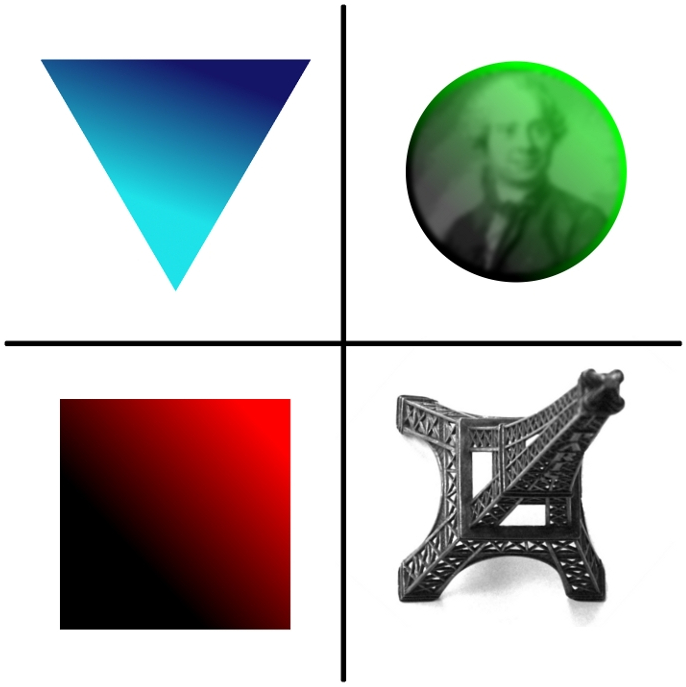
\includegraphics[height=2cm]{images/IJLRDA.jpg}\\
    \vspace{1cm}
      {\Large \@ED}\\
    \vspace{1cm}
      {\huge 
      	%{\bfseries \@doctorat}\\
    %\vspace{0.5cm}
      	TH\`{E}SE}\\
    \vspace{1cm}
   		{\bfseries pour obtenir le grade de docteur délivré par}\\
    \vspace{1cm}
    	{\huge\bfseries \@ecole}\\
    \vspace{0.5cm}
    	{\Large{\bfseries Spécialité doctorale “\@specialite''}}\\
    \vspace{1.2cm}
    	\textit{présentée et soutenue publiquement par}\\
    \vspace{0.5cm}
    	{\Large {\bfseries \@author}} \\
    \vspace{0.5cm}
    	le \@date \\
    \vfill
       {\LARGE \color[rgb]{0,0,0.4} \bfseries{\@title}} \\
\vspace{0.2cm}
       {\large \color[rgb]{0,0,0.4}{\@subtitle}}\\ 
    \vfill
        Directeur de thèse : {\bfseries \@directeur}\\
        Co-encadrant de thèse : {\bfseries \@encadrant}\\
    \vfill
	\begin{tabular}{>{\bfseries}lll}
		\large Jury\\
		\@jurya
		\@juryb
		\@juryc
		\@juryd
		\@jurye
		\@juryf
		\@juryg
		\@juryh
		\@juryi
	\end{tabular}
	\vfill
	
	\@adresse
  \end{titlepage}




\restoregeometry  
}


\author{Sagar \textsc{Pal}}
\title{Investigation of complex liquid-gas interfacial flows}
\subtitle{A numerical study using advanced Volume-of-Fluid methods}
\ED{ \'{E}cole doctorale n$^\circ$ 391 : Sciences m\'{e}canique, acoustique, \'{e}lectronique et robotique de Paris (SMAER)}
\doctorat{Doctorat Sorbonne}
\specialite{M\'{e}canique}
\directeur{St\'{e}phane \textsc{Zaleski}}
\encadrant{Daniel \textsc{Fuster}}
\date{29 septembre 2020}
\jurya{M. Jean-Luc Estivalezes}{Ma\^{i}tre de Recherche, ONERA}{Rapporteur}
\juryb{Mme. Lydia Bourouiba}{Associate Professor, MIT}{Rapporteur}
\juryc{M. Heinz Pitsch}{Professor, RWTH Aachen}{Examinateur}
\juryd{M. St\'{e}phane Popinet}{Directeur de Recherche, CNRS}{Examinateur}
\ecole{Sorbonne Universit\'{e}}
\adresse{
	\textbf{Institut Jean le Rond $\partial$ 'Alembert} \\
	UMR CNRS 7190, Campus Pierre et Marie Curie, Paris , France
}

\begin{document}
\pagedegarde

%----------------------------------------------------------------------------------------
%	BOOK INFORMATION
%----------------------------------------------------------------------------------------

%\titlehead{PhD Thesis}
%%\subject{Use this document as a template}
%
%\title[]{Investigation of complex liquid-gas interfacial flows}
%
%\subtitle{A numerical study using \\ advanced Volume-of-Fluid methods}
%
%\author[]{Sagar Pal}
%
%\date{\today}
%
%\publishers{Institut Jean le Rond $\partial$'Alembert \\ Sorbonne Universit\'e}

%----------------------------------------------------------------------------------------

\frontmatter % Denotes the start of the pre-document content, uses roman numerals


%----------------------------------------------------------------------------------------
%	OPENING PAGE
%----------------------------------------------------------------------------------------
%
%\makeatletter
%\extratitle{
%	% In the title page, the title is vspaced by 9.5\baselineskip
%	\vspace*{9\baselineskip}
%	\vspace*{\parskip}
%	\begin{center}
%		% In the title page, \huge is set after the komafont for title
%		\usekomafont{title}\huge\@title
%	\end{center}
%}
%\makeatother
%
%----------------------------------------------------------------------------------------
%	COPYRIGHT PAGE
%----------------------------------------------------------------------------------------

%\extratitle{
%	% In the title page, the title is vspaced by 9.5\baselineskip
%	\vspace*{9\baselineskip}
%	\vspace*{\parskip}
%	\begin{center}
%		% In the title page, \huge is set after the komafont for title
%		\usekomafont{title}\huge Acknowledgement \\ 
%	\end{center}
%}
%
%\blindtext

%
%----------------------------------------------------------------------------------------
%	DEDICATION
%----------------------------------------------------------------------------------------

%\dedication{
%	The harmony of the world is made manifest in Form and Number, and the heart and soul and all the poetry of Natural Philosophy are embodied in the concept of mathematical beauty.\\
%	\flushright -- D'Arcy Wentworth Thompson
%}

%----------------------------------------------------------------------------------------
%	OUTPUT TITLE PAGE AND PREVIOUS
%----------------------------------------------------------------------------------------

% Note that \maketitle outputs the pages before here

% If twoside=false, \uppertitleback and \lowertitleback are not printed
% To overcome this issue, we set twoside=semi just before printing the title pages, and set it back to false just after the title pages
\KOMAoptions{twoside=semi}
%\maketitle
\KOMAoptions{twoside=false}

%----------------------------------------------------------------------------------------
%	PREFACE
%----------------------------------------------------------------------------------------

\chapter*{Acknowledgement}
\addcontentsline{toc}{chapter}{Acknowledgement} % Add the preface to the table of contents as a chapter

I am of the opinion that every \LaTeX\xspace geek, at least once during 
his life, feels the need to create his or her own class: this is what 
happened to me and here is the result, which, however, should be seen as 
a work still in progress. Actually, this class is not completely 
original, but it is a blend of all the best ideas that I have found in a 
number of guides, tutorials, blogs and tex.stackexchange.com posts. In 
particular, the main ideas come from two sources:

\begin{itemize}
	\item \href{https://3d.bk.tudelft.nl/ken/en/}{Ken Arroyo Ohori}'s 
	\href{https://3d.bk.tudelft.nl/ken/en/nl/ken/en/2016/04/17/a-1.5-column-layout-in-latex.html}{Doctoral 
	Thesis}, which served, with the author's permission, as a backbone 
	for the implementation of this class;
	\item The 
		\href{https://github.com/Tufte-LaTeX/tufte-latex}{Tufte-Latex 
			Class}, which was a model for the style.
\end{itemize}

The first chapter of this book is introductive and covers the most 
essential features of the class. Next, there is a bunch of chapters 
devoted to all the commands and environments that you may use in writing 
a book; in particular, it will be explained how to add notes, figures 
and tables, and references. The second part deals with the page layout 
and design, as well as additional features like coloured boxes and 
theorem environments.

I started writing this class as an experiment, and as such it should be 
regarded. Since it has always been indended for my personal use, it may 
not be perfect but I find it quite satisfactory for the use I want to 
make of it. I share this work in the hope that someone might find here 
the inspiration for writing his or her own class.

\begin{flushright}
	\textit{Federico Marotta}
\end{flushright}


%----------------------------------------------------------------------------------------
%	TABLE OF CONTENTS & LIST OF FIGURES/TABLES
%----------------------------------------------------------------------------------------

\begingroup % Local scope for the following commands

% Define the style for the TOC, LOF, and LOT
%\setstretch{1} % Uncomment to modify line spacing in the ToC
%\hypersetup{linkcolor=blue} % Uncomment to set the colour of links in the ToC
\setlength{\textheight}{23cm} % Manually adjust the height of the ToC pages

% Turn on compatibility mode for the etoc package
\etocstandarddisplaystyle % "toc display" as if etoc was not loaded
\etocstandardlines % toc lines as if etoc was not loaded

\tableofcontents % Output the table of contents

%\listoffigures % Output the list of figures

% Comment both of the following lines to have the LOF and the LOT on different pages
\let\cleardoublepage\bigskip
\let\clearpage\bigskip

%\listoftables % Output the list of tables

\endgroup

%----------------------------------------------------------------------------------------
%	MAIN BODY
%----------------------------------------------------------------------------------------

\mainmatter % Denotes the start of the main document content, resets page numbering and uses arabic numbers
\setchapterstyle{kao} % Choose the default chapter heading style

\setchapterpreamble[u]{\margintoc}
\chapter{Introduction} 
\labch{intro}

% Importance of multiphase interfacial flows 
\begin{marginfigure}
\centering
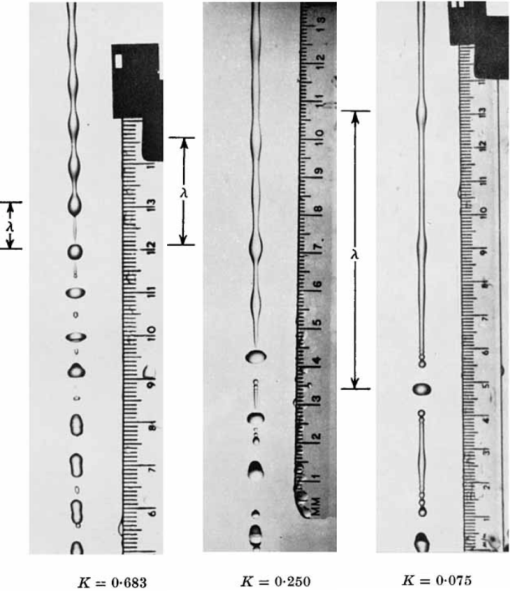
\includegraphics{plots/intro/jet.pdf}
\caption{Decay of a liquid jet into droplets due to the growth of capillary instabilities corresponding 
	to different excitation frequencies. Image reproduced from Rutland and Jameson \cite{rutland1971non}.
	} 
\label{jet}
\end{marginfigure}

The dynamics of liquid-gas interfacial flows play a critical role in several processes in nature, 
as well as in myriad industrial applications. 
The key elements of surface tension dominated flows such as droplets and bubbles constitute the  
fundamental mechanisms governing the exchange of heat and mass at the ocean-atmosphere interface \cite{seinfeld1998air,deike}, 
mixing/separation in context of metallurgical processes \cite{johansen1988fluid,metal},  
conventional modes of heat transfer \cite{deckwer1980mechanism,bubble}
and ever so importantly, the tranmission of pathogens \cite{lydia_1,lydia_2}. 
One of the most fascinating features of multiphase flows is the process of atomization, 
in which a liquid volume transitions into smaller fragments via a series of topological 
changes of varying complexity, ultimately resulting in the emergence of drops of various sizes
driven by the action of capillary forces at the interface separating the fluids.  
Such processes are ubiquitous in a diverse range of applications spanning from combustion related processes 
(\cite{lefebvre2017atomization,bayvel1993liquid}) to agricultural irrigation (\cite{lake1977effect,reichenberger2007mitigation}).    

% Decay of jets, shear induced atomization, expansion of sheets , hole expansion in sheets, secondary atomization of drops 

\begin{marginfigure}
\centering
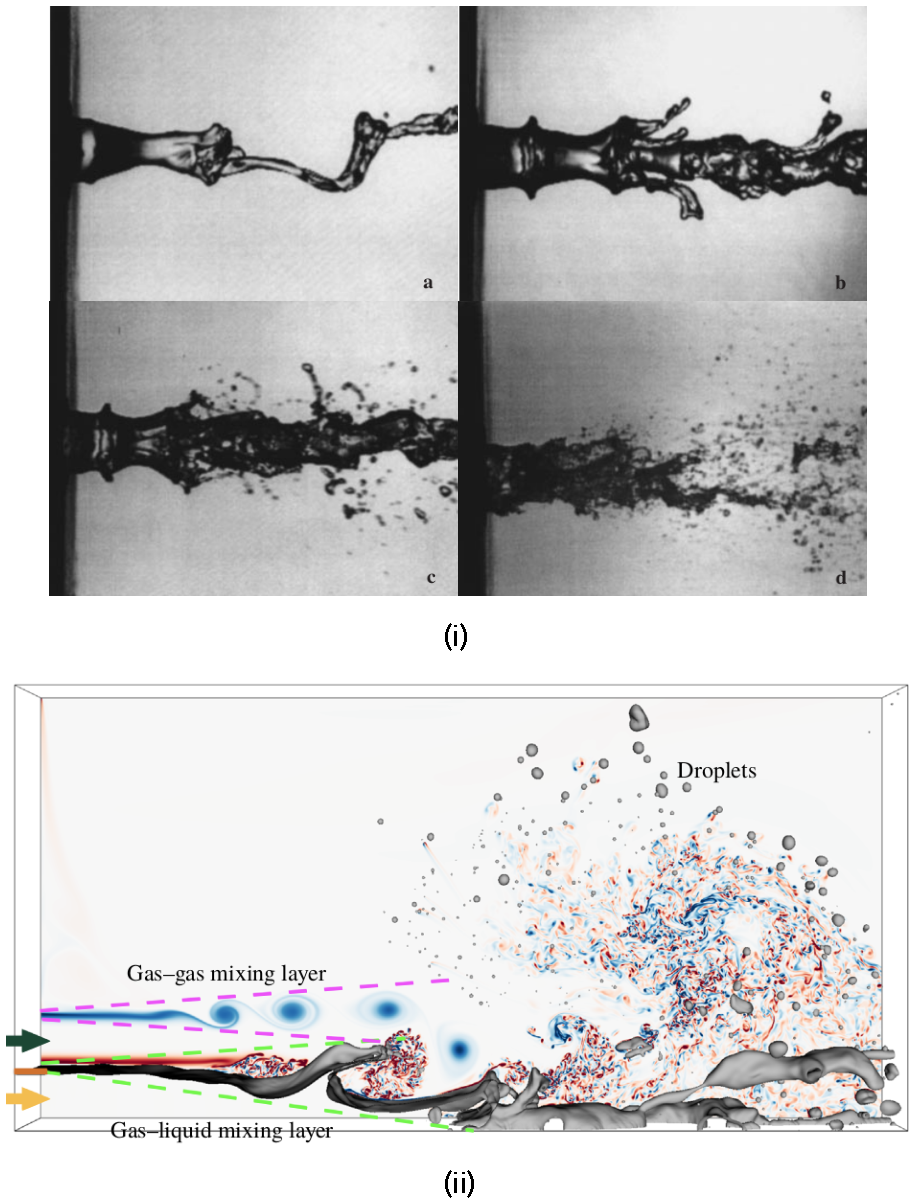
\includegraphics{plots/intro/shear.pdf}
	\caption{ Experimental (i) and numerical (ii) investigations of liquid atomization 
	in which the primary stages of topological change are driven by shear instabilities. 
	(i) Jet disintegration due to a high speed coaxial gas flow, image reproduced from Lasheras and Hopfinger \cite{lasheras}.
	(ii) Atomization of a two-phase mixing layer between parallel liquid and gas streams, image 
	reproduced from Ling et al. \cite{ling}.
	}
\label{shear}
\end{marginfigure}

\section*{Challenges in Numerical Modeling}

% Utility of numerical simulations, general info on interfacial tracking, Navier-Stokes 

% Artifical Atomization at low resolutions (raindrop crashes).

% Literature review of different attempts at momcons + summary tables

% Our Approach 


\section*{Polydispersity in Drop Sizes}

% Ligament mediated paradigm
% Breakup Regimes : Keller-Miksis inviscid, Paparouglou viscous, Eggers universal (inertio-visco) 

% Log-Normal, Gamma , Poisson distributions and underlying mechanisms

% Our approach


% Summary of parts and chapters in thesis


\pagelayout{wide} % No margins
\addpart{Numerical Development}

\pagelayout{margin} % Restore margins

\setchapterpreamble[u]{\margintoc}
\chapter{Methodology}
\labch{momcons}
 
In this chapter, we describe the our numerical methodology behind modeling 
the dynamics of immiscible incompressible liquid-gas interfacial flows under isothermal conditions. 
The numerical implementation is based on finite volume discretizations on uniform Cartesian grids, 
utilizing state of the art methods in interfacial reconstruction coupled with geometric
transport of the corresponding fluxes, curvature computation and surface tension modeling. 
A detailed exposition of our class of mass-momentum consistent numerical methods is provided, 
which are specifically designed to circumvent or suppress the uncontrolled and rapid  
growth of numerical instabilities that arise when dealing with flows entailing marked density contrasts . 
The implementations of the algorithms are developed on the free and open-source 
numerical platform called `PARIS Simulator' \cite{paris}, with the detailed descriptions 
of the general capabilities of the solver to be found in the previously cited reference. 

\section{Governing Equations}

We use the one-fluid formulation for our system of governing equations, thus solving 
the incompressible Navier-Stokes equations throughout the whole domain including regions 
of variable density and viscosity, which itself depend on the explicit 
location of the interface separating the two fluids.
In the absence of mass tranfer, the velocity field is continuous across
the interface at the incompressible limit, with the interface evolving according to the local velocity vector.  
Thus, the equations are as follows :  

% in incompressible flows, the velocity field is continuous in the absence of mass transfer across the interface 

\begin{align} 
	\frac{\partial \rho}{\partial t} + \nabla\cdot \left(\rho\boldsymbol{u}\right) &= 0 \label{mass} \\
	\frac{\partial}{\partial t} \left(\rho\boldsymbol{u}\right) + \nabla \cdot \left(\rho\boldsymbol{u}\otimes\boldsymbol{u}\right)  &= -\nabla p + \nabla \cdot \left(2 \mu \boldsymbol{D}\right) + \sigma \kappa \delta_{s}\boldsymbol{n} + \rho \boldsymbol{g}
\label{nseqn}
\end{align}


with $\rho$ and $\mu$ being the density and dynamical viscosity respectively. 
The volumetric sources are modeled by the acceleration $g$, and the 
deformation rate tensor $\boldsymbol{D}$ used to model the viscous stresses is defined as:  

\begin{align}
	\boldsymbol{D} = \frac{1}{2}\left[\nabla \boldsymbol{u} + \left(\nabla \boldsymbol{u}\right)^{T}\right]  
\end{align}


The term $\sigma \kappa \delta_{s}\boldsymbol{n}$ models the surface tension forces in the 
framework of the continuum surface-force (CSF) method. The normal vector to the interface 
is $\boldsymbol{n}$, with $\sigma$ being the coefficient of surface tension and $\kappa$ the 
local interfacial curvature. The operator $\delta_{s}$ is the Dirac delta function, 
the numerical approximation of which allows us to map the singular surface force distribution
along the interface onto their volumetric equivalents for our Cartesian control volumes. 
At the incompressible limit, the advection of mass given by equation \ref{mass} can be 
treated as equivalent to that of the advection of volume.

\subsection*{Material Properties}

Within the framework of interface capturing schemes, the 
temporal evolution of the interface separating the two fluids
can be tracked by the following advection equation : 

\begin{align} 
	\frac{\partial \chi}{\partial t} + \boldsymbol{u}\nabla\chi = 0 	
\label{chi}
\end{align}

where $\chi$ is the phase-characteristic function, that has different values 
in each phase \sidenote{Generally, $\chi$ is assigned values of $0$ in one phase and $1$ in the other. } . Mathematically, the function $\chi$
is equivalent to a Heaviside function in space and time. 
At the macroscopic length scales under consideration, the interface evolution
as described by equation \ref{chi} is modeled as having infinitesimal thickness
under the continuum hypothesis. The coupling of the interfacial evolution with
the equations of fluid motion as described in \ref{mass} and \ref{nseqn} is provided by :  

\begin{align}
	\rho &= \rho_{1}\chi + \left(1 - \chi\right)\rho_{2} \label {rho_chi} \\ 
	\mu  &= \mu_{1}\chi  + \left(1 - \chi\right)\mu_{2}  
  \label{mu_chi}
\end{align}

where $\rho_{1}$, $\rho_{2}$ are the densities of fluids 1 and 2 respectively, 
likewise for viscosities $\mu_{1}$ and $\mu_{2}$. For certain flow configurations, 
it might be beneficial to opt for a weighted harmonic mean description of the 
variable dynamic viscosity \sidecite{harmonic_mean}, instead of the weighted arithmetic mean as in equation \ref{mu_chi}. 

The two main (and most popular)
approaches in the context of interface capturing schemes are the 
volume-of-fluid (VOF) method first developed by Hirt and Nichols \cite{hirt1981volume}, 
and the level set class of methods pioneered by Osher and Sethian \cite{osher1988fronts}.
The principal difference between the two approaches lies in the manner in which
the Heaviside function $\chi$ is modeled in the discrete sense, 
either as a smooth differentiable field in
the case of level sets, or as a sharp discontinuous field in the volume-of-fluid (VOF) context.  
Each class of methods has its own set of merits (and demerits) relative to each other. 
Generally speaking, volume-of-fluid based methods display superior mass conservation
\sidenote{VOF based methods implicitly track the evolution of the discontinuous density field, 
which is not the case in level set based methods. }
whereas in terms of interface curvature computation, level set based methods hold an advantage
\sidenote{The differentiable nature of the level set function lends itself
to straightforward curvature computation routines. } . 
A detailed exposition into the different classes of interfacial transport
methods can be found in the seminal monograph by Tryggvason, Scardovelli and Zaleski \cite{zaleskibook}

%--------------------------------------------------------------------------------------------------------------------------
%--------------------------------------------------------------------------------------------------------------------------


\section{Interfacial Transport : VOF}

Our numerical studies are based on the Volume-of-Fluid methodology. 
We refer to the discontinuous approximation to the Heaviside function
\sidenote{A comprehensive discussion about the different types of approximations
to the interface Heaviside function can be found in Popinet \cite{popinet2018numerical}}
$\chi$ as the volume fraction field or colour function interchageably, which 
is defined below in the context of finite volume discretization : 

\begin{align} 
	C_{ijk}\left(t\right) = \frac{1}{\Delta V} \displaystyle\int_{\Delta V} \chi(\boldsymbol{x},t) \,d\boldsymbol x 
\end{align}

where $C$ is the colour function with its values lying between $0$ and $1$, 
with $i$,$j$ and $k$ being the indices to the corresponding discretized control volume of volume $\Delta V$.  
There are two steps involved in the VOF method, the reconstruction of the interface and its 
subsequent propagation (advection). We present a brief overview of the two steps in the following sections,
as going into detailed descriptions of the reconstruction and propagation procedures are 
not the focus of the present body of work \sidenote{In-depth explanations into these numerical 
techniques can be found in \cite{zaleskibook, zaleskiannual,vof_1,vof_2}.}.  


\subsection*{PLIC representation}
We use geometric reconstructions to explicitly define the 
interface location using the discrete colour function information. 
The interface is represented by disjointed line segments under 
the PLIC (piecewise linear interface construction)
framework as illustrated in figure \ref{vof_plic}, with the images reproduced 
from the the review by Scardovelli and Zaleski \sidecite{zaleskiannual}. 
Such reconstructions involve the determination of interface normals 
using the Mixed Youngs Centered method, the detailed description 
of which can be found in \cite{zaleskibook}. 

\begin{figure}[!h]
\begin{center}
\begin{tabular}{cc}
\hspace*{-1.0cm}
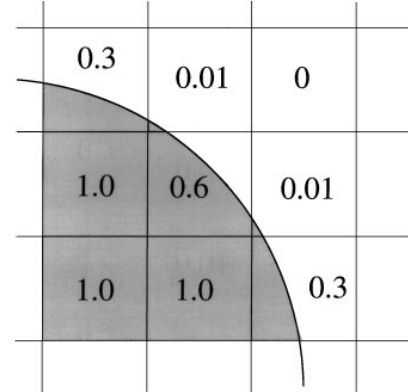
\includegraphics[width=0.5\textwidth]{plots/methodology/vof_basic.png} &
\hspace{-0.2cm}%
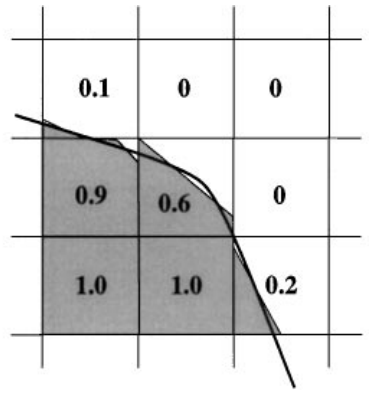
\includegraphics[width=0.473\textwidth]{plots/methodology/vof_plic.png} \\ 
\hspace{-0.2cm}%
(a) & (b) \\
\end{tabular}
\end{center}
\caption{ Exlicit definition of the interface location using the volume-of-fluid approach. 
These images are reproduced with permission from Scardovelli and Zaleski \cite{zaleskiannual}.
(a) The exact discrete representation of a circular arc on a regular Cartesian grid using the colour function field (volume fraction).
(b) The piecewise linear (PLIC) approximation to the smooth circular arc shown in (a), which entails second-order spatial accuracy.   
}
\label{vof_plic}
\end{figure}

\subsection*{Flux Computation}
Once the geometric PLIC reconstructions have been carried out, 
the interface segments are advected using the the velocity field. 
This entails computation of fluxes of the colour function, which 
can be computed via algebraic transport schemes (generally less accurate), 
or by using geometric reconstructions in either Eulerian, Lagrangian or hybrid frameworks.
In the context of our numerical platforms (`PARIS' and `Basilisk'), 
state-of-the-art \sidenote{The reader can refer to 
\cite{paris,basilisk} for further details}  
geometrical flux reconstruction procedues are utilised. 
The temporal integration of the fluxes could be carried out either as a 
series of one dimensional propagations along each of the spatial directions, 
termed as direction-split, or carried out in one single sweep, 
termed as multidimensional or unsplit.

Direction-split methods are more intuitive and easier to develop 
(extension of the one dimensional algorithm to 3D), 
but suffer from lack of conservation (to the order of 
machine precision) when it comes to 3D \sidenote{
A detailed exposition of this problem along with a noteworthy solution  
can be found in the work by Weymouth and Yue \cite{wy}}. 
Multidimensional (unsplit) methods have an advantage in that respect due to the 
fact that they are conservative by nature of their design, but are inherently 
more complicated to develop and implement, with no straightforward extension from 2D to 3D.    
For a more detailed and nuanced evaluation of the comparitive advantages of 
interfacial transport methods, we refer the reader to the recent review by 
Mirjalili et al. \cite{mirjalili2017interface} on the given subject.     
The propagation of the interface can be described by the evolution of
the colour function (volume fraction field) as  

\begin{align} 
	\frac{\partial C}{\partial t} + \boldsymbol{u} \cdot \nabla C = 0  	
\label{cvof_non}
\end{align}

We can express the left hand side of \eqref{cvof_non} in the conservative form as  

\begin{align} 
	\frac{\partial C}{\partial t} + \nabla \cdot \left(C \boldsymbol{u}\right) = C \left(\nabla \cdot \boldsymbol{u}\right) 	
\label{cvof_con}
\end{align}

As one can observe, the ``compression'' term on the right hand side of equation 
\ref{cvof_con} equals to zero in the context of incompressible flows without mass 
transfer, but it is important to keep this term in our numerical formulation within 
the direction-split framework. Discretization of the above equation results in :

\begin{align}
	C_{i,j,k}^{n,d+1} = C_{i,j,k}^{n,d} - F_{+}^{n,d}\left(C \right) - F_{-}^{n,d}\left(C \right) + \overline{C}_{i,j,k}^{n,d}\left(\frac{\Delta u_q}{\Delta x}\right)^{n,d}_{i,j,k}  
  \label{cvof_discrete}
\end{align}

The above equation represents an advection substep, the superscripts $n$ and $d$ refer to the timestep and 
direction of integration respectively. The notation $d=0$ refers to the field 
at the $n^{th}$ timestep, before any integration is performed along any direction. 
The fluxes $F_{\pm}^{n,d}(C)$ in equation \ref{cvof_discrete} are derived through geometrical reconstructions
\sidenote{For details regarding geometric flux reconstruction, refer to \cite{zaleskibook, zaleskiannual}}.
The $+$ and $-$ subcripts refer to the orientation with respect to the central cell ($i,j,k$).
The subscript $q$ refers to the direction corresponding to that given advection substep 
i.e either $X$, $Y$ or $Z$. In our case, our numerical platforms are based on cubic 
(regular Cartesian) grids, consequently there is no requirement for a subscript with $\Delta x$. 
After each substep, the interface is reconstructed once again with the updated 
volume fraction field in order to compute the fluxes for the next advection substep.  
Finally, the volume fraction field for the next timestep is given by 

\begin{align}
	 C^{n+1}_{i,j,k} = C^{n,3}_{i,j,k}  
\end{align}

The interpretation and numerical approximation of the prefactor $\overline{C}_{i,j,k}^{n,d}$ 
to the directional divergence, as well as the fluxes $F_{\pm}^{n,d}(C)$, depend 
on the exact nature of the geometrical advection scheme in question, 
which in our context is either CIAM (Lagrangian explicit) or Weymouth-Yue (Eulerian implicit) 
\sidenote{The classification of Lagrangian explicit and Eulerian implicit 
are in accordance with the paper by Aulisa et al. \cite{aulisa2003}}.
A brief outline of these two methods is presented in the subsequent sections.   

\paragraph{Lagrangian Explicit} 
This scheme was originally described in the work of Li \cite{li95}, `CIAM' being an 
abbreviation for the French title `\textit{Calcul d'interface affine par morceaux}', 
which can be thought of as a straightforward Lagrangian transport of the interface Heaviside function. 
After the interface segments are reconstructed from the discrete colour function 
at the start of the time-step, the interfacial points are transported by the component of the 
velocity field corresponding to the direction of transport. A geometrical interpretation of the scheme
is illustrated in figure \ref{fig:ciam}, reproduced from the seminal work of Gueyffier et al. \cite{gueyffier}. 

\begin{figure}[!h]
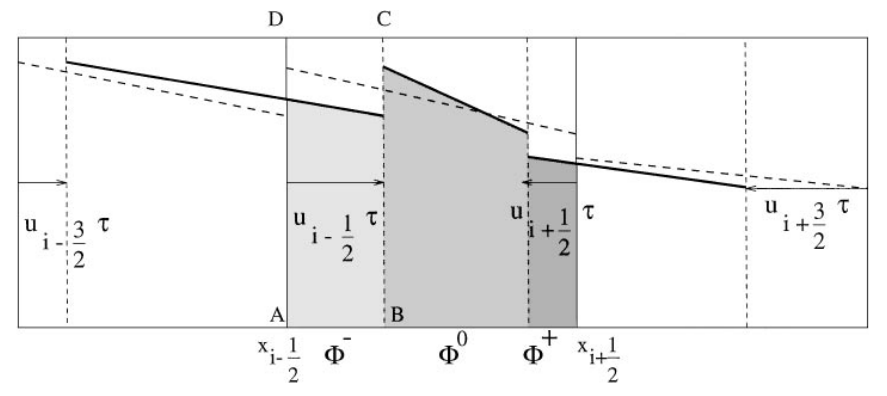
\includegraphics[width=1.0\textwidth]{plots/methodology/ciam.png} 
\caption{
Lagrangian transport of the interface segments using the CIAM scheme, the image
is reproduced with permission from Gueyffier et al. \cite{gueyffier}. 
A 2D schemetic of the geometric calculation of the fluxes of the volume 
fraction field is shown, for the advection substep along the horizontal direction.
The central cell ($i,j,k$) undergoes a net compression during this substep.
The fluxes $\Phi^{-}$ , $\Phi^{0}$ and $\Phi^{+}$ are the volumes under the 
advected interface segments advected by the interpolated velocity field,
intersected by the $(i,j,k)$ cell boundaries.
}
\label{fig:ciam}
\end{figure}

As one can infer from the geometrical representation in figure \ref{fig:ciam}, 
the fluxes $F_{\pm}^{n,d}(C)$ correspond to the volumes $\Phi^{-}$ and $\Phi^{+}$. 
Thus, the updated field $C_{i,j,k}^{n,d+1}$ is the sum of the 
three contributions $\Phi^{-}$ , $\Phi^{0}$ and $\Phi^{+}$. 
We can rewrite equation \ref{cvof_discrete} specifically for the CIAM scheme as   

\begin{align}
C_{i,j,k}^{n,d+1} =  C_{i,j,k}^{n,d}\left[1 + \left(\frac{\Delta u_q}{\Delta x}\right)^{n,d}_{i,j,k} \right] - F_{+}^{n,d}\left(C \right) - F_{-}^{n,d}\left(C \right)   
\label{ciam_discrete}
\end{align}

where the compression coefficient $\overline{C}_{i,j,k}^{n,d}$ is simply equal 
to the value of the colour function $C_{i,j,k}^{n,d}$ at the start of the 
corresponding advection substep. Although the flux terms cancel upon integration 
throughout the whole domain, one can clearly see that the compression terms do 
not sum up to zero due to the changing prefactor in front of the directional divergences. 
This precise issue brings us to the next advection scheme.      

\paragraph{Eulerian Implicit}
This advection scheme was developed by Weymouth and Yue \cite{wy} in order to 
specifically tackle the problem of discrete conservation when it comes to direction-split 
geometrical advection schemes \sidenote{By `discrete conservation' we mean that the sum of 
the directional divergences sum upto zero, to the accuracy of machine precision.}. 
The scheme fundamentally employs a forward Eulerian method in order to carry out temporal 
integration of the fluxes, with the fluxes themselves computed as the quantity of the substance 
entering or exiting a given control volume through its fixed surfaces, as shown in figure \ref{fig:wy}. 
This is in contrast with the flux computation method in the case of CIAM, 
where the interface segments are propagated forward in time in a Lagrangian fashion. 

\begin{figure}[!h]
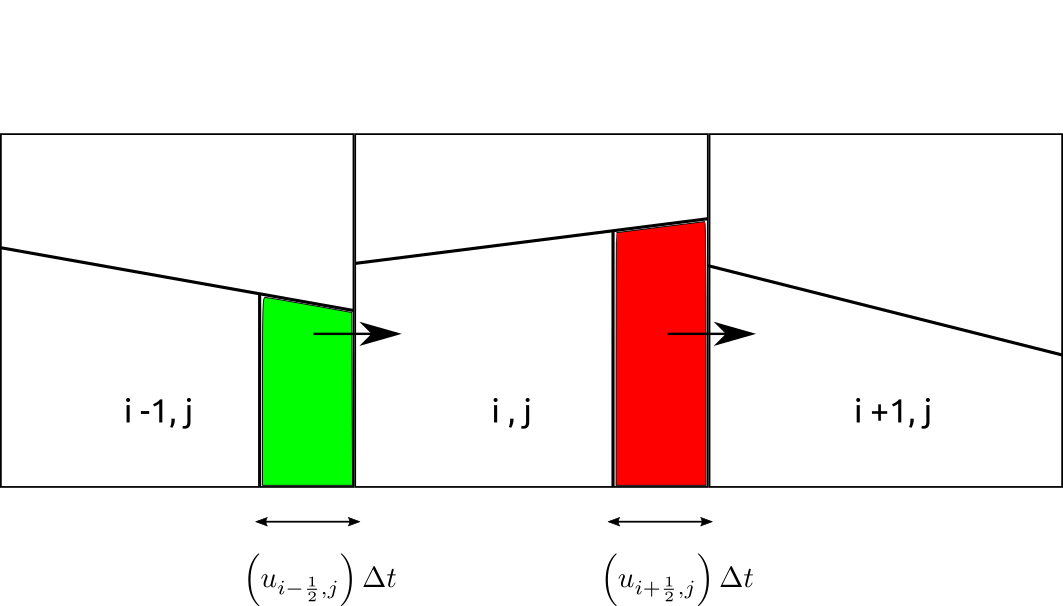
\includegraphics[width=1.0\textwidth]{plots/methodology/wy.png} 
\caption{ A 2D schemetic of the Eulerian (geometric) flux calculation  
using the Weymouth-Yue \cite{wy} scheme for the advection substep
along the horizontal direction, with the interface reconstructed 
using the volume fraction field at the start of the substep.
The colour fraction of the central cell ($i,j$) is updated during this substep
through the addition of the fluxes (coloured regions), with the green polygon corresponding
to the volume entering the cell $i,j$ from the $i-1,j$ and the red one corresponding to
that exiting $i,j$ into $i+1,j$. The geometric flux calculations are made on the basis
of the interfacial positions at the start of the substep, and the face centered velocities 
of the cell in question.}
\label{fig:wy}
\end{figure}

The subtle but important tactic used in this scheme lies in the manner in which the 
prefactor to the compression term \sidenote{Compression coefficient is used 
as a short-hand version of 'prefactor to the compression term'.}  is treated, with its definition being : 

\begin{align}
\overline{C}_{i,j,k}^{n,d} = H \left( C_{i,j,k}^{n,0} - 1/2 \right)
\label{wy_cond}
\end{align}

where $H$ is a one-dimensional Heaviside function. This renders the compression coefficient 
independent of the direction of the advection substep, consequently enabling the 
three discrete directional divergences to sum up to zero \sidenote{In numerical terms, we
can only ensure that they sum up to the accuracy of the Poisson solver $\sim 10^{-3} - 10^{-6}$
, with the limiting factor being the level of machine accuracy ($\sim 10^{-14} - 10^{-17}$). }
Therefore, the scheme is able to demonstrate volume conservation, subject to local 
CFL restrictions \sidenote{For a proof of discrete volume conservation subject to certain
CFL criteria, refer to the appendix of Weymouth and Yue \cite{wy}.}. To summarise, we can rewrite equation \ref{cvof_discrete}
for the Weymouth-Yue scheme as  

\begin{align}
C_{i,j,k}^{n,d+1} =  C \left[1 + \left(\frac{\Delta u_q}{\Delta x}\right)^{n,d}_{i,j,k} \right] - F_{+}^{n,d}\left(C \right) - F_{-}^{n,d}\left(C \right)   
\label{wy_discrete}
\end{align}

where $C$ is a constant with a value of either $0$ or $1$, determined by the value of $C_{i,j,k}^{n,0}$ according to equation \ref{wy_cond}.  

%--------------------------------------------------------------------------------------------------------------------------
%--------------------------------------------------------------------------------------------------------------------------

\section{Consistent Transport of Mass and Momentum}

Generally, we have a choice regarding how to discretize 
the convective operator of the incompressible Navier-Stokes equations. 
There is a well established corpus of numerical methods tailored specifically 
to deal with the non-conservative \sidenote{also referred to as the strong form, necessitating certain orders of smoothness of the primitive variable} form of the convective 
operator that appears in the transport equations of mass and momentum 
\sidenote{These methods are descendants of the class of numerical schemes used to solve hyperbolic partial differential equations.}
, which perform quite well in the context of single phase flows.
However, in interfacial flows we often deal with sharp discontinuities that 
arise as a consequence of the contrast in material properties between the two fluids. 
Therefore, even though the velocity field remains continuous throughout the domain, 
the otherwise smooth density (mass) and momentum fields 
contain sharp jumps localized at the interfacial position.     
Therefore, in regions of constant density and and viscosity, the standard non-conservative
form of the Navier-Stokes equations are discretized, whereas the discretization is
reformulated in a conservative form at locations in the vicinity of the interface.  

\subsection*{Spatiotemporal Discretization}

We start by describing the spatial arrangement of our
primary variables i.e. pressure ($p$) and velocity ($u_q$),
where $q = 1,2,3$ represents the $x$,$y$ and $z$ componenets respectively.
The control volume is in the form of a cube (3D) or a square (2D). 
The pressure and velocity variables are defined in a staggered arrangement, 
which means that the control volumes correpesponding to the velocity components 
$u_1$ and $u_2$ are shifted with respect to the control volume for pressure.
The staggered grid with the primary variables are represented in Figure \ref{stag-grid}.
The use of staggered control volumes has the advantage of
suppressing neutral modes (pressure oscillations) often observed in 
collocated methods but leads to more complex discretizations 
\sidenote{Refer to \cite{zaleskibook} for a more detailed discussion.}. 

In order to describe the overall numerical algorithm for the one-fluid 
Navier-Stokes equations with variable density and viscosity, 
we choose to the reframe our equations in a more convenient operator form, as presented below : 

\begin{align}
   \frac{\partial}{\partial t} \left( \rho \boldsymbol{u} \right) = L\left( \rho,\boldsymbol{u} \right) - \nabla p
\end{align}

The operator $L$ in the above expression can be decomposed as : 

\begin{align}
	L = L_{\textrm{adv}} + L_{\mu} + L_{\sigma} + L_{\textrm{g}} 
   \label{opr}
\end{align}

where the $L_{\textrm{adv}}$ represents the conservative advection, 
$L_{\mu}$ represents the diffusive forces generated by viscous stresses,
$L_{\sigma}$ represents the capillary forces arising from the surface tension model
and finally $L_{g}$ represents the volumetric (body forces) source term. 


\begin{figure}
\begin{center}
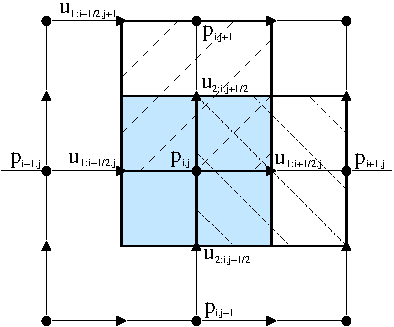
\includegraphics[width=\textwidth]{plots/stag-grid.pdf}
\end{center}
\caption{A 2D schematic of the staggered spatial configuration of the
pressure and velocity variables.
The pressure $p_{i,j}$ is based on the center of its control volume (light colour area);
the horizontal velocity component $u_{1;i+1/2,j}$ is defined in the middle of the
right edge of the pressure control volume and centered on its control volume
(dash-dotted area); the vertical velocity component $u_{2;i,j+1/2}$ is defined in the
middle of the top edge and centered on its corresponding control volume (dashed area).
The volume fraction is defined at the same location as that of the pressure, 
resulting in pressure and density being centered on identical control volumes.  
}
\label{stag-grid}
\end{figure}

We apply the spatially discretized versions of these operators (denoted by the superscript $h$) 
onto the primary variables ($C,\boldsymbol{u}$), and march forward in time using a small, 
possibly variable time-step $\tau$ such that $t_{n+1} = t_{n} + \tau$. 
In the first part of the algorithm, the volume fraction field $C^{n}$ is updated to the next timestep 
, with the superscript $n$ signifying discretization in time. 
The operation can be written as follows        

\begin{align}
	C^{n+1} = C^{n} + \tau L^{h}_{\textrm{vof}}\left( C^{n},\boldsymbol{u}^{n}\right)  
\label{cvof_update}
\end{align}

\marginnote{
The subscripts $i,j,k$ are dropped in equations \eqref{cvof_update} 
and \eqref{mom_update}, with the understanding that the operators in 
equation \ref{opr} apply uniformly to all control volumes. 
}

The temporal evolution of the volume fraction field represented above by the 
operator $L^{h}_{\textrm{vof}}$ is in accordance with the Lagrangian explicit or Eulerian implicit 
advection schemes, as described in the previous sections. 
Once we have obtained the updated field $C^{n+1}$, we can move on to 
the temporal update of our momentum field given by 

\begin{align}
	\rho^{n+1}\cdot \boldsymbol{u}^{*} &= \rho^{n}\cdot \boldsymbol{u}^{n} + \tau L^{h}_{\textrm{adv}}\left( C^{n},\boldsymbol{u}^{n} \right) + \nonumber \\
				      & \tau \left[ L^{h}_{\mu}\left(C^{n+1},\boldsymbol{u}^{n}\right) + L^{h}_{\sigma}\left(C^{n+1}\right) + L^{h}_{\textrm{g}}\left(C^{n+1}\right)\right]
\label{mom_update}
\end{align}

In regions of constant density. the advection operator $L^{h}_{\textrm{adv}}$ 
is implemented using higher order spatial schemes 
coupled with a choice of non-linear flux limiters such as 
QUICK, ENO, WENO, Superbee, Verstappen and BCG.
\sidenote{These high-order spatial schemes are based on well established methods 
developed to deal with hyperbolic conservation laws, for more details refer to the 
studies of Leveque \cite{flim_1} and Sweby \cite{flim_2}.}. 
For control volumes in the vicinity of the interface location, we revert to lower order 
schemes due to the sharp jumps in the material properties across the interface.  
The functionality of the operator $L^{h}_{\textrm{adv}}$ near the interface is tighly coupled
to that of $L^{h}_{\textrm{vof}}$ from equation \ref{cvof_update}, 
so as to ensure consistency in the discrete advection of mass and momentum.
The details regarding this coupling shall be the focus of this section. 

\subsection*{Advection of Conserved Quantities}

\newcommand{\dert}[1]{\frac{\partial #1}{\partial t}}
\newcommand{\cijk}{C_{i,j,k}}
\newcommand{\pijk}{\phi_{i,j,k}}
\newcommand{\X}{\boldsymbol{x}}
\newcommand{\N}{\boldsymbol{n}}
\newcommand{\rijk}{\rho_{i,j,k}}
\newcommand\mijk{(\rho u_{q})_{i,j,k}}

We start with the advection of the interface position, which in 
the VOF framework is given by - 

\marginnote{In the VOF approach, the approximation to the interface Heaviside 
function contains a sharp discontinuity, in contrast to the level set approach 
where the approximation is continuous in the discrete sense.}


\begin{align}
	\dert H + \nabla \cdot (\boldsymbol{u} H) = H\, \left(\nabla \cdot \boldsymbol{u} \right) \,
	\label{heaviside}
\end{align}


Integrating this equation in time after carrying 
out spatial discretization, one obtains -    


\marginnote{$\cijk^n$ is the colour function or volume fraction field at time step $n$ 
obtained through the finite volume discretization of the interface Heaviside function.}


\begin{align}
{\cijk^{n+1} - \cijk^{n}} = - \sum_{\textrm{faces} \, f} F^{(c)}_f + \int_{t_n}^{t_{n+1}}  
	{\textrm{d}}t \int_\Omega  H \, \left(\nabla \cdot \boldsymbol{u}\right) \,  {\textrm {d}}\X   \,,
\label{sumf}
\end{align}


where the first term on the right-hand side is the summation over the cell faces $f$  
of the fluxes $F^{(c)}_f$   
\sidenote{These fluxes of $(\boldsymbol{u} H)$ are computed via geometrical reconstructions,
and not via high-order non-linear interpolation schemes which are 
the standard (in the absence of discontinuities) . } . 
As one can clearly observe, the ``compression'' term on the 
right-hand side of equation \eqref{heaviside} disappears for incompressible flow, 
however it is essential in the context of direction-split geometric advection schemes.
The definition of the geometric fluxes in mathematical form is -  

\begin{align}
	F_f^{(c)} = \int_{t_n}^{t_{n+1}} {\textrm {d}}t \int_{f} u_f(\X,t) H(\X,t) \, {\textrm{d}}\X \,,
\label{faceint}
\end{align}

where $u_f = \boldsymbol{u}\cdot \N_f$ 
\sidenote{Component of the velocity normal to the control surface $f$.}.
Once an approximation for the evolution of $(\boldsymbol{u} H)$ during
the time step is chosen, a four-dimensional integral remains to be
computed in equation (\ref{faceint}).
The advection schemes used are CIAM and Weymouth-Yue, which have been 
described in the previous section. 
Directional splitting results in the breakdown of equation (\ref{sumf}) 
into three equations, one for each advection substep -


\begin{align}
{\cijk^{n,l+1} - \cijk^{n,l}} = - F^{(c)}_{m-} - F^{(c)}_{m+} 
+ c_m \partial_{m}^h u_m \,,
\label{sumf2}
\end{align}


\marginnote{The superscript $l=0,1,2$ is the substep index, i.e.
$\cijk^{n,0} = \cijk^{n}$ and $\cijk^{n,3} = \cijk^{n+1}$. 
The face with subscript $m-$ is the ``left'' face in direction $m$ with 
$F^{(c)}_{m-} \ge 0$ if the flow is locally from right to left. A similar reasoning 
applies to the ``right'' face $m+$.}

After each advection substep (\ref{sumf2}), the interface is reconstructed
with the updated volumes $\cijk^{n,l+1}$, then the 
fluxes $F^{(c)}_{f}$ are computed for the next substep. 
Importantly, we have approximated the compression term in (\ref{sumf}) by -

\begin{align}
	\int_{t_n}^{t_{n+1}}  {\textrm {d}}t \int_\Omega  H \partial_m u_m  {\textrm {d}}\X \simeq  c_m 
 \partial_{m}^h u_m \, 
 \label{comp}
\end{align}

\marginnote{There is no implicit summation carried out 
over $m$, and the superscript $h$
denotes the spatial discretization of the operator. } 

On the right hand sides of (\ref{sumf2}) and (\ref{comp}) 
the flux terms $F_{f}^{(c)}$ and the 
 partial derivative $\partial_{m} u_m$ must
be evaluated using identical discretized velocities.
The expression $\partial_{m}^h u_m$ is a finite volume approximation of the 
spatial derivative corresponding to the $m$th component 
of the velocity vector along direction $m$, and
the ``compression coefficient'' $c_m$ approximates the color fraction. 
Its exact expression is dependent on the advection method
\sidenote{Refer to chapter \ref{ch:method} to see the difference in
the definitions of the compression coefficient between  
the CIAM and Weymouth-Yue methods.}
and it also entails the desirable property of $C$-bracketing
\sidenote{The preservation of $0 \le \cijk \le 1$ 
is referred to as $C$-bracketing. }. 
Due to the possible dependence of the 
compression coefficient $c_m$ on the Cartesian direction
corresponding to the advection substep, 
the sum $\sum_m c_m \partial_{m}^h u_m$ may not necessarily vanish
even if the flow is incompressible.
As mentioned previously, the main appeal of the Weymouth-Yue method 
is its ability to keep this sum to zero, within the limits of machine precision. 
In order to achieve consistent transport of the discontinuous fields 
of mass and momentum, we start by trying to understand the advection 
of a generic \textit{conserved} scalar quantity $\phi$ by a continuous velocity field - 


\begin{align}
	\dert \phi + \nabla \cdot \left( \phi \, \boldsymbol{u} \right)  = 0 
\label{phiconv}
\end{align}


where the field $\phi$ is smoothly varying except 
at the interface position, where it may be discontinuous.
The essence of this study lies in the search of a scheme that  
propagates this discontinuity ($\phi$) at the same speed as 
that of the advection of volume fraction ($C$).

\marginnote{The smoothness of the advected quantity away from the interface
is verified for fields such as density $\rho$, momentum $\rho \boldsymbol{u}$ 
and internal energy $\rho e$.}

Temporal integration of the spatially discretized version of \eqref{phiconv} gives us - 

\begin{align}
\pijk^{n+1} - \pijk^{n} = - \sum_{\textrm{faces}\, f} F^{(\phi)}_f 
\label{sumfp}
\end{align}

\marginnote{The sum on the right-hand side is the sum over faces $f$ of cell $i,j,k$ 
of the fluxes $F^{(\phi)}_f$ of $\phi$, which are defined as the color function fluxes
$F^{(c)}_f$ in \eqref{faceint}.}


where the fluxes are defined as -

\begin{align}
	F_f^{(\phi)} = \int_{t_n}^{t_{n+1}} {\textrm {d}}t \int_{f} u_f(\X,t) \,\phi(\X,t) \,
	{\textrm {d}}\X
\label{pfaceint}
\end{align}

In order to ``extract'' the discontinuity we introduce the 
 interface Heaviside function $ H(\X,t) $

\begin{align}
F_f^{(\phi)} = 
\int_{t_n}^{t_{n+1}} {\textrm d}t \int_{f} \left[ u_f  \,H \,\phi  +  u_f \,(1-H) \,\phi \right] 
\, {\textrm d}\X \, 
\label{fluxphi}
\end{align}

Therefore, the flux can be decomposed into two components as -

\begin{align}
F_f^{(\phi)} = 
\bar \phi_1 \int_{t_n}^{t_{n+1}} {\textrm d}t \int_{f} u_f \,H \,{\textrm d}\X + 
\bar \phi_2 \int_{t_n}^{t_{n+1}} {\textrm d}t \int_{f} u_f \,(1-H) \,{\textrm d}\X \,,
\label{barphi}
\end{align}

where the face averages $\bar \phi_s$, $s=1,2$, are defined as - 


\begin{align} 
\bar \phi_s = \frac{\int_{t_n}^{t_{n+1}} {\textrm d}t \int_{f} \phi \,u_f \,H_s  
{\textrm d}\X}{\int_{t_n}^{t_{n+1}} {\textrm d}t \int_{f}  
u_f \,H_s\,{\textrm d}\X} \,,  
\label{barphi2}
\end{align}


and $H_1=H$, $H_2= 1-H$. 
The total flux can be rearranged as a sum of the constituents 
corresponding to the different `fluids' - 

\marginnote{Expression \eqref{barphi} can be written in terms 
of the fluxes $F^{(c)}_f$ and $F^{(1-c)}_f$, this second one being obtained by 
replacing $H$ with $1-H$ in \eqref{faceint}}

\begin{align}
F_f^{(\phi)} = \bar \phi_1 \,F_f^{(c)} +  \bar \phi_2 \,F_f^{(1-c)} \,.
\label{fluxphi12}
\end{align}



\subsubsection*{Advection of Density}
% VOF - rho consistency with compression term etc

The density field $\rho(\X,t)$ follows the 
temporal evolution of the generic conserved quantity
(\ref{phiconv}) by setting $\phi = \rho$. 
At the incompressible limit the velocity field is 
solenoidal (divergence-free), with constant densities 
in each phase. We can extract the density trivially from the integrals 
\eqref{barphi2} to \textit{exactly} obtain $\bar \rho_s = \rho_s$. 
The flux definitions corresponding to $\rho$ become    


\begin{align}
F_f^{(\rho)} = \rho_1 F_f^{(c)} +  \rho_2 F_f^{(1-c)}
\label{fluxrho}
\end{align}

\marginnote{We use the term `conservative' to express the fact
that eq. (\ref{sumfp}) computes the temporal evolution of $\rho$ 
as a difference of fluxes, instead of velocity times its gradient.}


Using the above definitions for density fluxes,
one can employ any VOF method to construct fluxes of the color 
function in order to obtain conservative transport for $\rho$
In principle, this should result in the conservation of total mass.  
However, as we have already pointed out the fact that the CIAM
method does not conserve volume exactly 
\sidenote{This again comes back to the dependence of the compression 
coefficient on the volume fraction field at the start of each
advection substep.}
, consequently, the advection of the density field (mass) 
is not consistent with that of the advection of $C$. 

This apparent paradox is resolved by including the 
compression term on the right hand side of \eqref{phiconv},
in order to ensure consistency. 
The advection equation for the conserved quantity now becomes - 


\begin{align}
\dert \phi + \nabla \cdot ( \phi \,\boldsymbol{u})  = \phi \, \left(\nabla \cdot \boldsymbol{u}\right) 
\label{phiconv2}
\end{align}


This equation can be decomposed into advection substeps corresponding to 
the direction-split integration framework as follows - 

\marginnote{The direction-split integration steps operations for $\phi$
mirror that of the volume fraction $C$. }


\begin{align}
{\pijk^{n,l+1} - \pijk^{n,l}} = - F^{(\phi)}_{m-} - F^{(\phi)}_{m+} 
+ \Big( \tilde \phi_1^m c^{(1)}_m + \tilde \phi_2^m c^{(2)}_m \Big) \, \partial_{m}^h u_m 
\label{sumfpconsistent}
\end{align}


\marginnote{$c^{(1)}_m=c_m$ is the compression coefficient corresponding 
to the particular VOF advection method for volume fraction $C$ ,
while $c^{(2)}_m= 1 -c_m$ corresponds to that of the 
symmetric color fraction  $1 - C$.}


The fluxes $F^{(\phi)}_{m\pm}$ follow the definition given in \eqref{fluxphi12}, 
, while the cell averages $\tilde \phi_s^m$ are defined as - 


\begin{align}
\tilde \phi_s^m = \frac{\int_{t_n}^{t_{n+1}} {\textrm{d}}t \int_{\Omega}  \phi  H_s  
\partial_{m}^h u_m  \,  {\textrm{d}}\X}
{\int_{t_n}^{t_{n+1}} {\textrm{d}}t \int_{\Omega} H_s  \partial_{m}^h u_m \,{\textrm{d}}\X} \,
\label{cellphi2}
\end{align}


Rewriting the direction-split integration operation for $\rho$ we get - 


\marginnote{In case of CIAM, the compression coefficient is defined as
$c_m = \cijk^{n,l}$, whereas in Weymouth-Yue the coefficient is independent
of the advection substep $l$, defined as  
$c_m = H\left(\cijk^{n} - 1/2 \right)$, where $H$ is the Heaviside function.}


\begin{align}
{\rijk^{n,l+1} - \rijk^{n,l}} = - F^{(\rho)}_{m-} - F^{(\rho)}_{m+} + C_m^{(\rho)}\,,
\label{sumfrho}
\end{align}


where the fluxes are given by (\ref{fluxrho}) and the compression term is

\marginnote{Again, there is no implicit summation rule on $m$.} 


\begin{align}
C_m^{(\rho)} =  \left( \rho_1 c^{(1)}_m + \rho_2 c^{(2)}_m \right) \,\partial_{m}^h u_m  
\label{central}
\end{align}



For the WY method, the compression terms eventually cancel upon 
summation over the substeps, therefore resulting in the conservation  
of mass at the same accuracy as the discrete incompressibility condition
$\sum_{m=1}^3 \partial_{m}^h u_m=0$ is verified 
\sidenote{This usually corresponds to the tolerance of the Poisson solver,
with a typical value being $10^{-6}$. }. 



\subsubsection*{Advection of Momentum}
% model of computing consistent mass-momentum fluxes

Within the framework of advection of a generic conserved scalar,
we consider momentum advection as transport of the scalar quantities  
$\phi=\rho u_q$, where $q=1,2,3$ is the component index. 
Using the definition given in \eqref{barphi2}, 
we obtain the expression -  

\marginnote{The expressions with the `bar' 
refer to face weighted averages of the varible in question. 
Here, $\bar \phi_s = \overline { \rho u_q}_s$ }


\begin{align} 
\overline{\rho u_q}_s = \rho_s \bar u_{q,s} 
\end{align}


where $\bar u_{q,s}$ is termed as the ``advected interpolated velocity'', 
whose precise definition is given as - 


\begin{align}
	\bar u_{q,s} =  \frac{\int_{t_n}^{t_{n+1}} {\textrm{d}}t \int_{f}  u_q u_f  H_s  \, {\textrm{d}}\X}{\int_{t_n}^{t_{n+1}} {\textrm{d}}t \int_{f}  u_f  H_s\,{\textrm{d}}\X} \label{barudef}
\end{align}

\marginnote{The subscript $s$ denotes the phase or fluid,
and $f$ represents the normal components defined on the face
centers.} 


Thus, the direction-split integration of the momentum can be represented as - 


\begin{align}
{\mijk^{n,l+1} - \mijk^{n,l}}  = - F^{(\rho u)}_{m-} - F^{(\rho u)}_{m+}
 + \Big( \rho_1 \tilde u_{q,1}^m  c^{(1)}_m +  \rho_2 \tilde u_{q,2}^m c^{(2)}_m 
 \Big) \, \partial_{m}^h u_m 
\label{sumfrou}
\end{align}


where the momentum fluxes are constructed in the following manner -


\begin{align}
 F^{(\rho u)}_{f} =  \rho_1 \,\bar u_{q,1}  \,F^{(c)}_{f}  +  
 \rho_2 \,\bar u_{q,2}  \,F^{(1-c)}_{f} \,,
\end{align}


The expression for the ``central interpolated velocity'' corresponding to the 
averages $\tilde \phi_s^m$ of \eqref{cellphi2} is -  

\marginnote{Notice that ``cloning'' the advected velocities 
$\bar u_{q,1}$ and $\bar u_{q,2}$ 
would make it easier to advect a velocity field 
with a jump on the interface, but would 
render the overall algorithm quite complicated. }


\begin{align}
	\tilde u_{q,s}^{m} = \frac{\int_{t_n}^{t_{n+1}} {\textrm{d}}t \int_{\Omega} u_q \, H_s \,  
	\partial_{m}^h u_m   \,  {\textrm{d}}\X}
	{\int_{t_n}^{t_{n+1}} {\textrm{d}}t \int_{\Omega} H_s \, \partial_{m}^h u_m \,{\textrm{d}}\X} 
\label{tildeudef}
\end{align}


The superscript $m$ is intentionally omitted  
for the velocities $\tilde u_q^m$ in order to avoid
cumbersome and complicated notations. 

\marginnote{Due to the viscous effects and 
the absence of phase change in our fluid dynamics model,   
the velocity filed maintains continuity across the interface.} 

As a reasonable approximation we choose to put 
$\bar u_q =  \bar u_{q,1} = \bar u_{q,2}$ for the 
``advected interpolated velocity'' and 
$\tilde u_q =  \tilde u_{q,1} = \tilde u_{q,2}$
for the ``central interpolated  velocity''. 
An important simplification which serves as  
the central model in our development is given by -  

\marginnote{To add clarity to the notion of ``central interpolated velocity'', 
one can understand this as the face-centered interpolations of the velocity field 
(component normal to control surface), which is required to compute the fluxes of volume. }


\begin{align}
 F^{(\rho u)}_{f} = \bar u_q F^{(\rho)}_{f} \label{frou}
\end{align}


Therefore, the advection substep for the momentum can finally we written as -   


\begin{align}
{\mijk^{n,l+1} - \mijk^{n,l}} =  -\bar u_q  F^{(\rho)}_{m-} - \bar u_q  F^{(\rho)}_{m+} 
+ \tilde u_q C_m^{(\rho)}
\label{sumfmom2}
\end{align}


where the density fluxes are defined in \eqref{fluxrho} and the compression term 
$C^{(\rho)}$ in \eqref{central}. 


\marginnote{ In the above expression the face-weighted 
average velocities $\bar u_q$ are defined
using (\ref{barudef}) on the corresponding
left face $m-$ or right face $m+$. 
}

Although the weighted averages $\bar u_q$ and $\tilde u_q$ have been defined,
the manner in which they are estimated shall be covered in the following section. 

In the context of the CIAM advection scheme, the compression coefficient
for the volume fraction field is $C^{n,l}$, similarly, for the 
central interpolated velocity we take $\tilde u_q = u_q^{n,l}$. 
Due to the summation of the directional divergences not cancelling out,
the resulting transport of the momentum field is not exactly conservative.
On the other hand, the compression coefficient is independent 
of the advection substep in the context of the Weymouth-Yue advection scheme. 
The final expression for the compression coefficient becomes - 

\marginnote{The Weymouth-Yue coefficient is a constant value $c$,
that is independent of direction $m$.}

\begin{align}
C_m^{(\rho)} =  \Big( \rho_1 c + \rho_2 (1-c ) \Big) \,\partial_{m}^h u_m  \,.
\label{central2}
\end{align}


Since there is no bracketing on any velocity component, 
we take $\tilde u_q = u_q^{n}$, which is independent of the substep $l$.


\marginnote{The compression terms sum up to  
the accuracy to which the solenoidal nature 
of the velocity field is discretely verified  
.}

The final expression after cancellation of the compression terms,
having undergone three advection substeps \eqref{sumfmom2} is  

\begin{align}
	{\mijk^{n,3} - \mijk^{n}} =  - \sum_{\textrm{faces} \, \textrm{f}}  \bar u_{q}  F^{(\rho)}_{f} . 
\label{sumfmomtotfracstep}
\end{align}


Therefore, the extension of the Weymouth-Yue mass (volume) 
advection scheme to the consistent
transport of momentum allows the discrete 
transport to be exactly conservative. 


\subsubsection*{Velocity Interpolations}

% computation of slope limiters with diagram, distinction in bulk and interfacial regions

The direction-split momentum transport given by \eqref{sumfmom2}
can be carried out in either of the bulk of the phases, or at
close proximity to the interface location. The treatment away 
from the interface is expressed as - 

\marginnote{
In the bulk, the expression simplifies considerably due to the 
density and volume fraction being constant, hence resulting in the
cancellation of the spurious compression terms. 
.}


\begin{align}
{u^{n,3}_q - u_q^{n}} =  - \sum_{\textrm{faces} \, \textrm{f}}  \bar u_{q} u_f 
\label{sumfmomtot}
\end{align}


Here, we distinguish between an ``advecting'' velocity 
$u_{f}= \boldsymbol{u} \cdot \N_f $
\sidenote{The ``advecting'' velocity computes the fluxes of volume fraction.},
and an ``advected velocity'' component $\bar u_{q,f}$, 
which is basically an average over the face $f$. 
Due to the momentum transport being carried out on 
staggered control volumes, both these velocity components
require some interpolations from their original positions
onto the necessary positions on the staggered grid.
Using this new nomenclature, \eqref{sumfmomtot} becomes -

\begin{align}
{u^{n,3}_q - u_q^{n}} =  - \sum_{\textrm{faces} \, \textrm{f}}  \bar u_{q}^{\textrm{(advected)}} 
u^{\textrm{(advecting)}}_f   
\label{sumfmomtotbulk}
\end{align}
	
Now, moving onto the approximation in the neighbourhood
of the interface, we get - 

\marginnote{
In the previous section we had derived a 
new expression for the momentum fluxes and the
compression term, i.e. the RHS of \eqref{advect-ed-ing-2}, 
that is consistent with the discrete transport of the volume fraction.  
.}


\begin{align}
	{(\rho u_q)^{n,3} - (\rho u_q)^{n}} =  - \sum_{\textrm{faces} \, \textrm{f}}  \bar u_{q}^{\textrm{(advected)}}  
F^{(\rho)}_{f} + \sum_{m=1}^3 \tilde u_q C_m^{(\rho)} \, 
\label{advect-ed-ing-2}
\end{align}


The crux of our model for momentum advection is described 
by these two equations (\eqref{sumfmomtotbulk} \& \eqref{advect-ed-ing-2}).
We start by pointing out the staggered spatial arrangement of our
primary variables (presssure, velocity, volume fraction), 
as illustrated by Fig. \ref{stag-grid} in a 2D representation.  
\sidenote{Figure \ref{stag-grid} has the same variables
arrangement that is found in 3D on a plane perpendicular to the $z$-axis and through the 
pressure point $p_{i,j,k}$. 
}


To estimate the advecting velocities $u_f^{\textrm{(advecting)}}$ we use a centered scheme.
Consider a face perpendicular to the horizontal direction $1$
\sidenote{
In particular , $f=1-$. 
}
There are two cases, the first corresponding to when 
the advected component is not aligned with the 
face normal, which is the case with $q=2$. 

\marginnote{
The $u_2$ control volume in Fig. \ref{stag-grid} is centered on $i,j+1/2,k$, and face $f=1-$ is then 
centered on $i-1/2,j+1/2,k$. 
}

The advecting velocity  $u_{1-}^{\textrm{(advecting)}}$ 
is not given on this point, therefore it has to be interpolated as - 


\begin{figure}
\begin{center}
    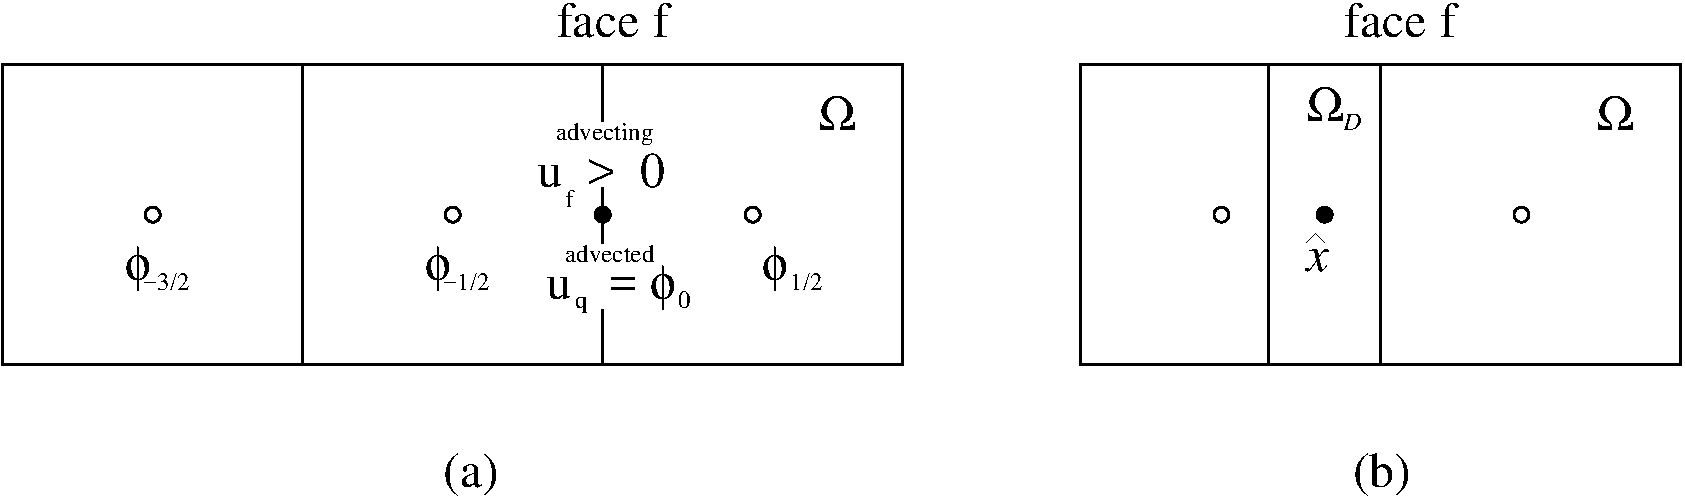
\includegraphics[width=\textwidth]{plots/advect-ed-ing.pdf}
\end{center}
\caption{The reference control volume $\Omega$ for the advected velocity component 
$\phi=u_q$ is shown. A horizontal advection is here considered and both the advecting velocity 
$u_f$ and the advected velocity require an interpolation for their value on the left face 
$f=1-$: (a) the value $\bar u_q = \phi_0$ (full circle) is interpolated 
(see \ref{appendix}) from the values $\phi=u_q$ on the nodes (open circles);
(b) a more sophisticated interpolation predicts the value $\phi(\hat x)$ where $\hat x$ is
at the center of the ``donating'' region $\Omega_D$ (see \ref{appendix}).}
\label{advect-ed-ing-fig}
\end{figure}




\begin{align}
 u_{1;i-1/2,j+1/2,k}^{\textrm{(advecting)}} = \frac12 \big( u_{1;i-1/2,j,k} + u_{1;i-1/2,j+1,k} 
\big) \,
\label{uf2}
\end{align}


In the second case the advected component is aligned with the 
face normal, corresponding to $q=1$. 
\marginnote{
The $u_1$ control volume 
in Fig. \ref{stag-grid} is centered on $i+1/2,j,k$ and face $f=1-$ is then 
centered on $i,j,k$.
}
In this case, the interpolation becomes -  


\begin{align}
	u_{1;i,j,k}^{\textrm{(advecting)}} = \frac12 \big( u_{1;i-1/2,j,k} + u_{1;i+1/2,j,k} \big) \,
\label{uf1} 
\end{align}
 

Thus far, we have covered only interpolations
concerning the ``advecting'' velocity, which is basically
used to compute fluxes of the volume fraction. 
Now we turn our attention to interpolations of the \textit{advected}
velocity $\bar u_{q}$ which appears in \eqref{advect-ed-ing-2}. 
\marginnote{
The interpolants we use in this case are
one-dimensional and operate on the velocities $u_q$, on the center of their 
control volumes, that are regularly spaced on a segment aligned 
with the direction of the advection, that is also perpendicular to face $f$. 
}
In Fig. \ref{advect-ed-ing-fig}, we demonstrate the principle 
behind our interpolation scheme along the horizontal direction $1$, 
with the lighter notation $\phi = u_q$.
The objective is to interpolate the ``advected'' velocity on the left face
of the reference control volume $\Omega$.
In case of advected velocity $u_1$ and the advecting velocity \eqref{uf1} on face
$f=1-$, the relationship with the $\phi$ values in Fig. \ref{advect-ed-ing-fig} is -


\begin{align}
\phi_{-3/2} = u_{1;i-3/2,j,k}, \quad \phi_{-1/2} = u_{1;i-1/2,j,k}, \quad   
\phi_{1/2} = u_{1;i+1/2,j,k}, \;\cdots
\end{align}


whereas in the case of the ``advected'' velocity $u_2$ and the advecting velocity \eqref{uf2},
the relationship turns out to be -


\begin{align}
\phi_{-3/2} = u_{2;i-2,j+1/2,k}, \quad  \phi_{-1/2} = u_{2;i-1,j+1/2,k}, 
\quad  \phi_{1/2} = u_{2;i,j+1/2,k}, \;\cdots
\end{align}

In order to get a prediction of $\phi_0$ on the 
face $f=1-$ in Fig. \ref{advect-ed-ing-fig}
\sidenote{ $\phi_0$ serves as an approximation of 
$\bar u_q$ given in \eqref{barudef}.
}
we use an interpolation function $f$ that computes 
this value as a function of the four nearest points,
and in an upwind manner based on the sign of the 
\textit{advecting} velocity $u_f$. Thus, the interpolation
can be expressed in functional form as - 

\marginnote{
The extension of these approximations to advection along 
the other two directions $q=2,3$ is straightforward. 
}

\begin{align}
\phi_0 = f \left( \phi_{-3/2}, \phi_{-1/2}, \phi_{1/2},\phi_{3/2},\textrm{sign}(u_f) \right)
\label{simpleinterp}
\end{align}


Throughout this body of work, we have extensively tested and used 
two variants of such interpolation functions, the exact implementation 
of which can be found in Appendix A. The interpolation functions are :


\marginnote{The reader can refer to influential works of 
LeVeque \cite{flim_1} and Sweby \cite{flim_2} regaring the role
of non-linear flux limiters such as QUICK, Superbee, WENO/ENO etc 
in the context of numerical methods for hyperbolic conservation laws. 
}

\begin{enumerate}
\item A scheme based on the QUICK 
third order interpolant in the bulk, away from the interface 
and a simple first order upwind flux near the interface. 
\item A scheme based on the Superbee slope limiter \sidecite{roe1985some} for the flux in the 
bulk and a modified Superbee limiter tuned to a shifted interpolation point near the 
interface.  
\end{enumerate}


\section{Advection on Staggered Grids}

The development of the consistent transport schemes should be integrated into
the broader context of our numerical algorithm which deals with the 
coupling between the conservative formulation of the 
one-fluid Navier-Stokes equations and the geometric transport of the interface.  
In this section, we describe two distinct strategies that we have implemented in order to achieve 
discrete consistency between mass (VOF) and momentum transport, specifically 
in the context of our staggered Cartesian grid (see Fig. \ref{stag-grid}). 


\subsection*{Shifted Fractions Method}
% algorithm, flow chart , how to reconstruct on shifted grid, lack of conservation 

This strategy tackles the problem of staggered control volumes by reconstructing 
\sidenote{The reconstructions involve geometrical operations, thus are not
easily translated into equations.}
the centered volume fraction field onto the staggered control volumes 
, thereby resulting in a field of \textit{shifted} fractions. 


\begin{figure}
\begin{center}
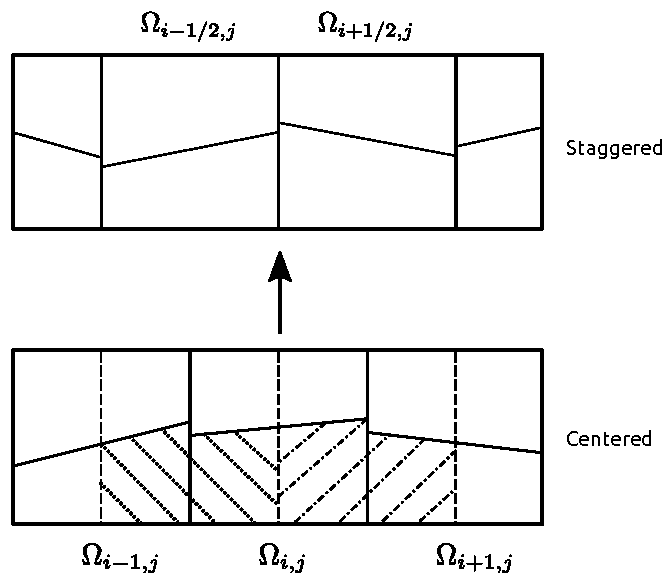
\includegraphics[width=\textwidth]{plots/shifted_fractions.pdf}
\end{center}
\caption{A 2D schematic of the reconstruction procedure 
used in the \textit{shifted fractions} method. 
In this case, advection of the horizontal component of momentum is considered.
The half-fractions from the centered control volumes 
$\Omega_{i,j}$ and $\Omega_{i+1,j}$ (dash-dotted area) are added together
to obtain the volume fraction in the shifted (staggered) volume $\Omega_{i+1/2,j}$.
Similarly, the half-fractions from $\Omega_{i-1,j}$ and $\Omega_{i,j}$ (dotted area)
are combined to obtain the volume fraction $\Omega_{i-1/2,j}$.
Once this horizontally shifted volume fraction field is reconstructed, 
the corresponding density, momentum and ``advected'' velocity fields can be 
computed in order to carry out consistent transport of mass and momentum
on this staggered configuration. 
}
\label{shift_frac}
\end{figure}


A 2D schematic of this reconstruction procedure is given in Fig. \ref{shift_frac} 
, considering the advection of the horizontal component of momentum. 
At the beginning of the operations summarized by $L_{\textrm{adv}}$, 
each velocity (momentum) control volume overlaps two pressure/VOF (centered)
control volumes i.e.  $\Omega_{i+1/2,j}$ overlaps $\Omega_{i,j}$ and $\Omega_{i+1,j}$
Therefore, the two half-fractions from $\Omega_{i,j}$ and $\Omega_{i+1,j}$ are 
added together to obtain an estimate
\sidenote{These estimations utilize the set of same set of geometric operations
that are used in the reconstruction of the interface and fluxed volumes.
.}
of the shifted fraction $C_{i+1/2,j}$ in $\Omega_{i+1/2,j}$. 
Once this key reconstruction step is carried out, the mass and momentum
fields, as well as their corresponding fluxes can all be derived using the information
from the shifted volume fraction field. These operations performed at each time step
are summarized in the following steps : 


\begin{enumerate}

\item Interface reconstruction at time $t_n$ using data $C^{n}$.
        
	\marginnote{$q=1,2,3$ is the component index, 
	e.g $\rho_1$ in $\Omega_{i+1/2,j,k}$ for the 
	horizontal momentum component $\rho_1 u_1$.
	}

\item Computation of half-fractions as shown in Fig. \ref{shift_frac},
	in order to obtain the ``shifted'' fraction field $C^{n}_q$ and $\rho^{n}_q$
	in the staggered control volumes.

\item Computation of all three momentum components $(\rho_q u_q)^{n}$
	at $t_n$.
	\marginnote{ The fluxes of momentum are derived from those of mass
		using the relation \eqref{frou} ,
		which in turn are obtained in a consistent fashion from 
		the fluxes corresponding to `shifted' volume fraction field.}

\item Advection of all three momentum components along one coordinate direction,
	say $x$ direction, using \eqref{sumfmom2} to obtain the updated momentum components
	$(\rho_q u_q)^{n,1}$ after the first substep.

\item Advection of the ``shifted'' density field $\rho^{n}_q$ on the staggered volumes 
	using VOF consistent advection, along the $x$ direction in order to
	 obtain the updated volume fractions after the first substep.

\item Extraction of the provisional velocity components 
	\sidenote{These provisional velocities are required
		to compute the ``advected'' velocities using 
		the non-linear flux limiters, as described in \eqref{advect-ed-ing-2}.}
	$u_q^{n,1}$ after the first substep, i.e. $u_q^{n,1} = (\rho_q u_q)^{n,1}/\rho_q^{n,1}$.

\item The above operations are repeated for the different momentum components, shifted
volume fractions and densities, and velocity components for the next two substeps
with split advections along the $y$ and $z$ directions.
\sidenote{At each time step, the sequence $x, y, z$ is permuted, in order to avoid 
any systematic biases in error propagation.}
Finally, we obtain $(\rho_q u_q)^{n+1} = (\rho_q u_q)^{n,3}$ and
$\tilde \rho_q^{n+1} = \rho_q^{n,3}$. 

\item In parallel, the centered volume fraction field $C^{n}$ 
	is advected in order to obtain $C^{n+1} = C^{n,3}$ using the VOF advection method. 

\end{enumerate}


\begin{figure}
\begin{center}
    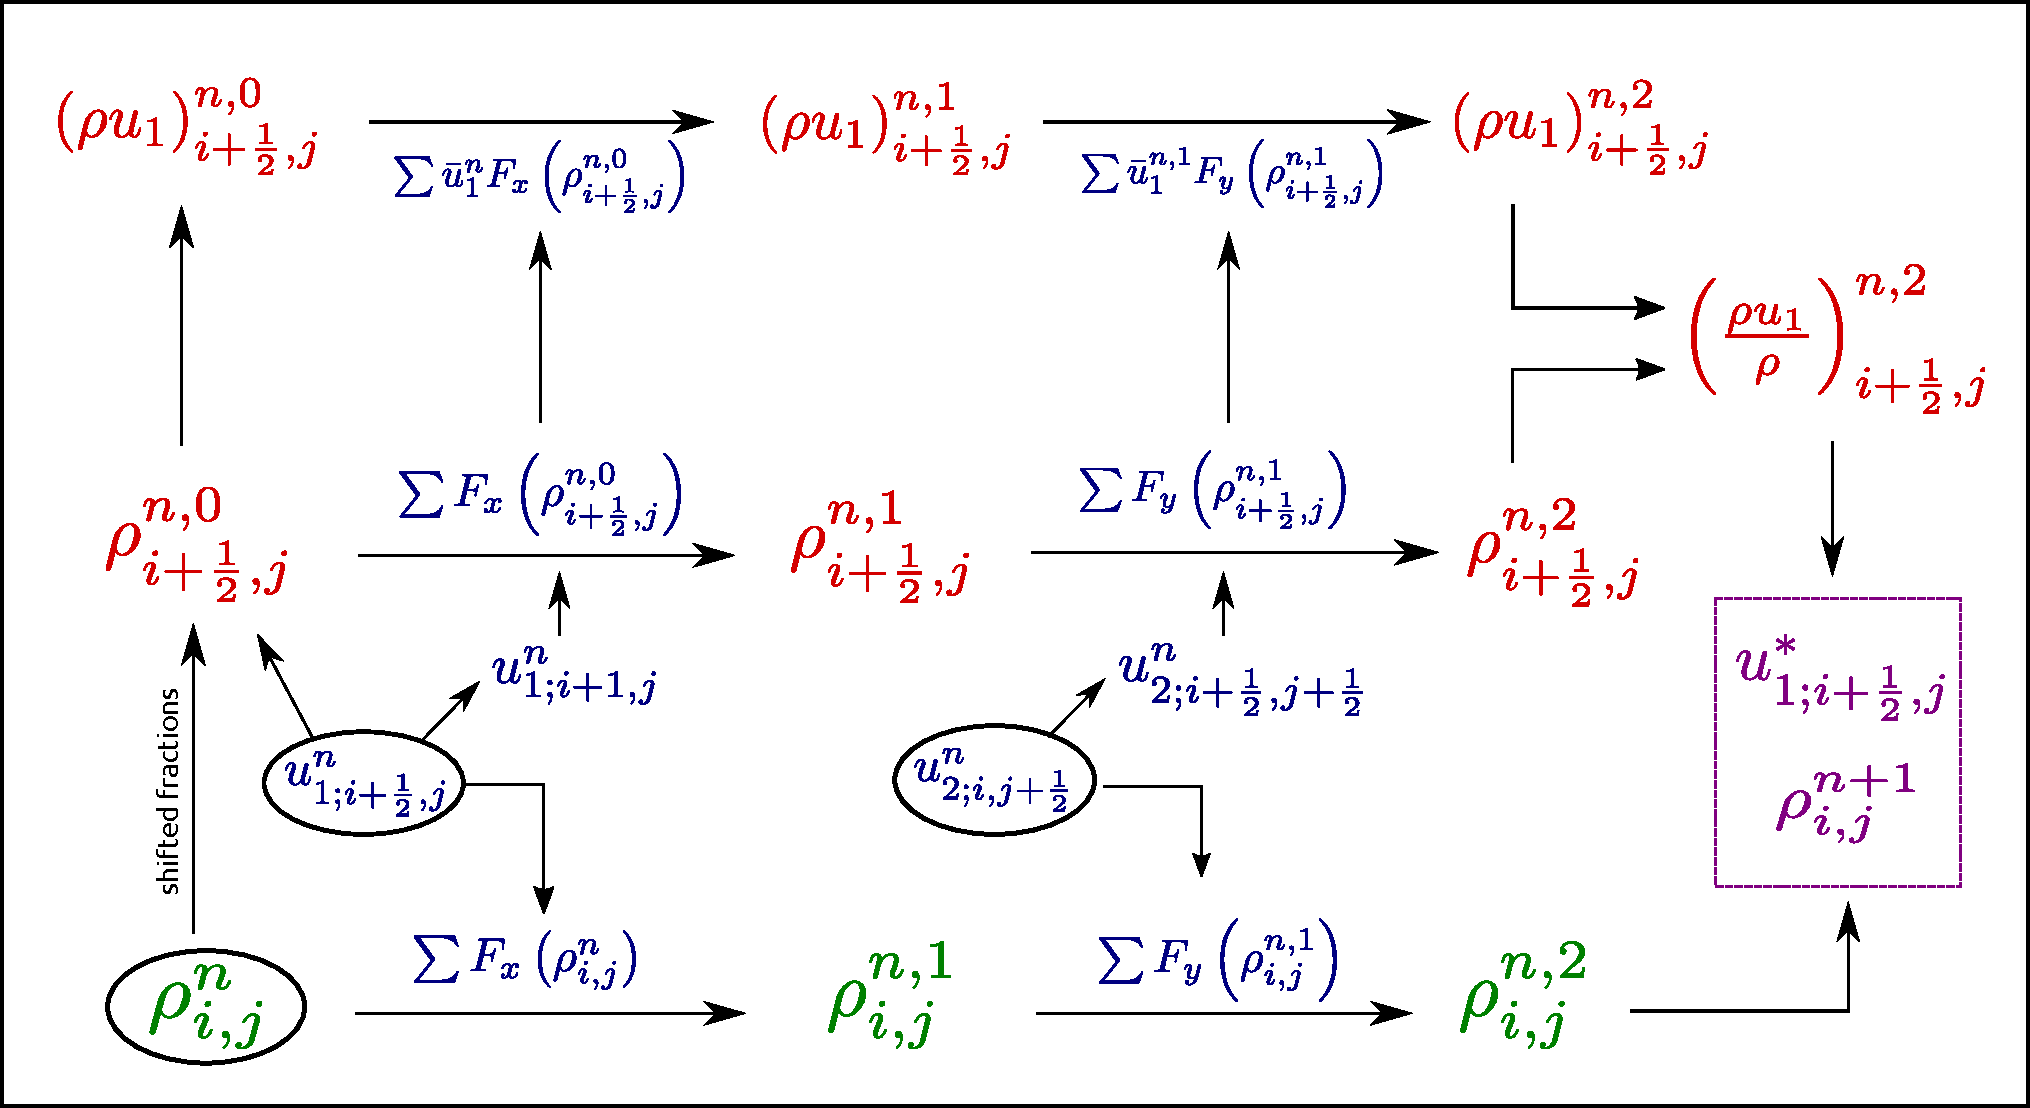
\includegraphics[width=\textwidth]{plots/momcons_diagram_daniel.pdf}
\end{center}
\caption{A bird's eye view of the \textit{shifted fractions} method,
highlighting the operations performed at each time step. 
This method achieves consistency in the discrete transport 
of mass and momentum on the staggered control volumes.
In the interest of brevity, we present a 2D case for the
density on the grid $i,j$ and horizontal velocity $u_1$ on the staggered grid $i+1/2,j$.
The evolution of the velocity component $u_2$ on the staggered grid $i,j+1/2$ is similar.
The initial variables $\rho^n$, $u_1^n$, $u_2^n$ are inside the ellipses. The interpolated
``advecting'' components $u_1$ and $u_2$ have superscript $n$. The shifted density $\rho^{n,0}$
is constructed with the shifted fractions of $C$ to initialize the momentum component
$(\rho u_1)^{n,0}$. The first split advection is along the $x$ direction  to 
variables with superscript $n,1$, the second one is along the $y$ direction to
variables with superscript $n,2$. The updated density is $\rho^{n,2}=\rho^{n+1}$
while the horizontal velocity $u_1^{n,2}=u_1^{*}$ enters the RHS of the Poisson-like
equation \ref{poisson}. }
\label{momcons_daniel}
\end{figure}


An important point to note from the above algorithm is that 
the advected velocity components $u_q$ are updated at each substep,
while the advecting velocities $u_f$ are interpolated from the initial
velocity field $\boldsymbol{u}^n$ at time $t_n$. 
The shifted fractions of Fig. \ref{shift_frac}
are computed using routines that are already part of our
geometrical toolbox, used primarily in flux computation. 


In essence, we have a consistent transport of density (mass)
and momentum on the staggered grids, while simultaneously 
carrying out advection of the volume fraction field on the centered grid. 
\marginnote{
A naive attempt to achieve momentum conservation could entail always using the 
shifted fields $C^{n}_{q}$ and evolve them by the VOF method on the staggered cells. 
Such an approach would render the scheme conservative, but would result in the  
independent evolution of the three staggered grids, eventually leading to divergence.
}
As a consequence, the momentum components $(\rho_q u_q)^{n+1}$ 
(at time step $t_{n+1}$) that are derived from the 
corresponding ``shifted'' volume fractions $C^{n+1}_q$ 
and densities $\rho^{n+1}_q$  (obtained from $C^{n+1}$)
are different from the densities $\tilde \rho_q^{n+1} = \rho_q^{n,3}$
, which were computed during the previous time step 
by directly advecting the ``shifted'' volume fractions $C^{n}_q$. 
The origin of this discrepancy is the approximate nature of the  
linear reconstruction of the interfaces, which is not 
even continuous on the boundary of its control volume.
Therefore, this implies that the momentum is not exactly
conserved between two time steps, even though the Weymouth-Yue method
ensures conservative transport of the momentum on the staggered control volumes. 


%--------------------------------------------------------------------------------------


\subsection*{Sub-Grid Method}

In this strategy, the difficulty associated with consistent 
transport on staggered control volumes is resolved by advecting  
the volume fraction (mass) on a twice finer grid 
\sidenote{
The grid is twice as fine when compared to the control volume for momentum.
} , very much in the spirit of Rudman's \cite{rudman1998volume} original work. 

The primary motivation regarding the development of this 
method is the issue of conservation (lack of) concerning 
the discrete transport of momentum in case of the shifted fractions method.     
Basically, the issue arises quite simply due to the fact that the volume fraction 
$C^{n+1}$ used to construct the staggered momentum field at the start of a 
new time step is \textit{not} the identical to that which is obtained 
via advection on the staggered control volumes itself ($C_{q}^{n+1}$). 
\sidenote{
In the shifted fractions method, flux computations on the staggered 
cells necessitate another round of interfacial reconstructions based on the shifted 
volume fraction field, whereas the sub-grid volume fraction information enables one
to circumvent the reconstructions and obtain the fluxes directly using simple surface integrals.
}
The sub-grid method is able to evade these complications that arise due to
the parallel evolution of two different volume fraction fields by conducting 
volume fraction on solely on the twice refined grid.  
An additional advantage of the having the sub-grid volume fraction field is that 
it facilitates a more `natural' computation of not only the staggered 
volume fraction field $C^{n+1}_q$, but more importantly its fluxes. 
This method is currently only compatible with the implicit fluxes 
computed in the Weymouth-Yue VOF advection method. 

Considering the overall approach, the \textit{key differences} between our 
present algorithm and the implementations in the 
original works of Rudman and Weymouth-Yue are : 

\begin{description}
	\item[Rudman (1998)\cite{rudman1998volume} ] The use of a conservative geometrical 
		mass (volume fraction) transport framework instead of an algebraic one in 
		the original method, which is applied to sub-grid volume fraction field.  
	\item[Weymouth \& Yue (2010) \cite{wy}] The extension of the 
		original method for conservative direction-split mass transport to the momentum field, 
		culminating in the discrete consistency between mass 
		momentum transport in the context of staggered Cartesian grids in 3D. 
\end{description}


\subsubsection*{Spatial Configuration : Coarse \& Sub-Grid Variables}

\begin{figure}[h!]
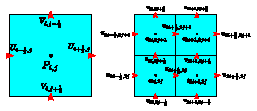
\includegraphics[width = \textwidth]{plots/sub_grid.pdf} 
\centering
\caption{A 2D schematic of the arrangement of primary variables 
on the coarse and sub-grid levels. 
The control volume is decomposed into the two figures, the one
on the left corresponding to the coarse grid variables, while the 
one on the right corresponding to the sub-grid. 
Superposition of these two figures, one on top of each other,
represent the spatial relationships between the two sets of variables.
The velocities on the sub-grid level are simple first 
or zeroth order interpolations of the coarse grid velocities.
}
\label{sub_grid}
\end{figure}

To start, we describe the spatial orientation of the different 
variables on the two refinement levels of the grid.   
\marginnote{The notations for the variables are slightly
different that those used in the previous sections (Fig. \ref{stag-grid}.) 
The velocity component in the horizontal and vertical directions 
are now denoted as $U$ and $V$ respectively, and the pressure by $p$. 
}
At the coarse grid level, the pressure and velocity fields are 
defined in a staggered configuration, with pressures at the cell 
centers (centroids in 3D) and velocities on the cell face centers. 
In Fig. \ref{sub_grid}, we demonstrate the arrangement of variables, 
which one can easily extrapolate to 3D during implementation, 
but for the sake of clarity we illustrate its 2D equivalent. 
The volume fraction $C$ 
\sidenote{ The volume fraction field $C$ is denoted as $c$ in Fig. \ref{sub_grid}. 
} is only defined on a grid that is twice as fine than 
that of the pressure/velocity grid, which we refer to as the sub-grid. 
Therefore in 3D, each cubic control volume is divided into eight constituent 
smaller cubic volumes at the centroids of which, the volume fraction field is centered. 


\subsubsection*{Multiscale Coupling : Restriction \& Prolongation Operations}

As is paradigmatic for dual-grid methods in the context of 
Navier-Stokes solvers, we carry out mass transport 
at the sub-grid level, and momentum transport at the coarse level. 
In pressure-projection based methods such as ours, the predominant 
bottleneck in terms of computational speed is the 
iterative solution to the discrete Poisson equation. 
\sidenote{
The problem size of such elliptical 
partial differential equations is governed by 
the number of cells/points discretizing the velocity (or pressure) field. 
If we choose to solve the problem on a mesh with
twice the resolution in 3D, that would lead to an 8 fold increase 
in the problem size for the discrete pressure-Poisson problem.   
}
Therefore, solving the mass advection equation on the fine grid 
allows us not only to obtain more accurate solutions to the flow physics 
involved, but also enables us to avoid the significantly higher  
computational costs associated with solving a Poisson problem 
at a twice finer resolution.  

\paragraph{\textbf{Prolongation}}

In order to advect the volume fraction at the sub-grid level, 
we need to reconstruct a velocity field at that level of resolution using 
information from the coarse grid velocity field.
\marginnote{ 
The prolongation operator has to be used at the start of each new time step,
in order to compute the sub-grid velocity field. 
}
In order to achieve this, we have implemented a prolongation operator 
which asserts the following relations between the velocities on the two refinement levels  

\begin{align}
  	  u_{2i-\frac{1}{2},2j} = u_{2i-\frac{1}{2},2j+1} &= U_{i-\frac{1}{2},j} \\ 
            u_{2i+\frac{3}{2},2j} = u_{2i+\frac{3}{2},2j+1} &= U_{i+\frac{1}{2},j} \\ 
  	  u_{2i+\frac{1}{2},2j} = u_{2i+\frac{1}{2},2j+1} &= \left(U_{i+\frac{1}{2},j} + U_{i-\frac{1}{2},j}\right) / 2 \\
  	  v_{2i,2j-\frac{1}{2}} = v_{2i+1,2j-\frac{1}{2}} &= V_{i,j+\frac{1}{2}} \\ 
            v_{2i,2j+\frac{3}{2}} = v_{2i+1,2j+\frac{3}{2}} &= V_{i,j-\frac{1}{2}} \\
  	  v_{2i,2j+\frac{1}{2}} = v_{2i+1,2j+\frac{1}{2}} &= \left(V_{i,j+\frac{1}{2}} + V_{i,j-\frac{1}{2}}\right) / 2 
\end{align}


The notations in the above equations refer to the description 
of the coarse and sub-grid variables in Fig. \ref{sub_grid}. 
The first-order interpolation applied to the coarse grid 
velocity field ensures discrete incompressibility 
\sidenote{This is a direct consequence of the solenoidal 
nature of the coarse grid velocity field.
}
at the sub-grid level.
The choice of interpolation order used in the  prolongation operator 
is identical to that of the originial method of Rudman (\cite{rudman1998volume}). 
In the current version of the sub-grid method, we have chosen to eschew the added 
complexity of solving local Poisson problems 
\sidenote{
The use of higher order interpolation schemes would necessitate 
finding the solutions of local Poisson problems, in order to 
render the sub-grid velocity field discretely divergence-free. 
}
through our prolongation operators, therefore sticking with 
the much simpler Rudman inspired interpolations. 


\paragraph{\textbf{Restriction}}


\begin{figure}[h!]
\centering
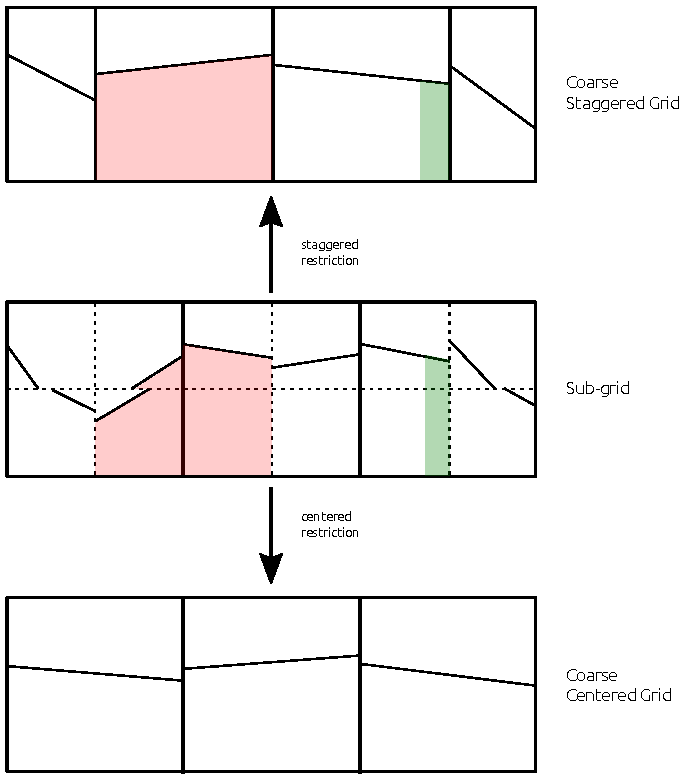
\includegraphics[width = \textwidth]{plots/subgrid_restriction.pdf}
\caption{A 2D illustration of the restriction operations involved
	between the different grid resolutions, where the sub-grid 
	grid boundaries are denoted by the dashed lines, 
	and that of the overlapping coarse grid by solid lines. 
	Restriction operations in the form of simple volume integrals
	are performed on the sub-grid volume fraction in order
	to compute the staggered and centered volume fraction 
	fields at the coarse grid level. 
	Restriction operators in the form of surface integrals 
	are also performed in order to compute the volume fluxes
	at the boundaries of the coarse staggered control volumes.
	The red shaded areas correspond to the volume fractions, 
	whereas the green shaded area corresponds to that of volume fluxes.
        The interface segments as depicted at the coarse grid level 
	are just for purpose of illustration, and are not
	`reconstructed'. Unlike the shifted fractions method, the 
	interfacial reconstructions on the staggered volumes are not 
	necessary, due to the fact that sub-grid volume fluxes are 
	simply combined to compute the staggered fluxes.  
	}
\label{restrict}
\end{figure}


In order to compute the required density and momentum fields
on the staggered grid (coarse level), we implement restriction operators
that use information from the sub-grid volume fraction field.  
\marginnote{
The restriction operators work in an identical manner as in 
Rudman (\cite{rudman1998volume}), which are nothing but simple volume 
integrals of the sub-grid field mapped onto the domains corresponding 
to the coarse grid control volumes. 
}
In Fig. \ref{restrict}, we demonstrate the different 
mappings between the two grid levels, which essentially boils down 
to volume integrals for the centered fields, and surface integrals 
for their corresponding fluxes.
A description of the different functions performed by the restriction 
operator is as follows : 

\begin{itemize}
	\item \textit{Fine Grid $\longmapsto$ Coarse Staggered Grid}
          
	  \begin{description}
		  \item[Density \& Momentum] The sub-grid volume fraction field
			  is restricted to obtain a staggered density field at the 
			  coarse grid level (see Fig. \ref{restrict}), which on combining with 
			  the appropriate component of the velocity field 
			  produces the staggered momentum field.    
		  \item[Fluxes] The geometric fluxes from the sub-grid volume fraction 
			field are restricted in order to obtain coarse grid fluxes for the 
			 corresponding staggered volumes, which on combining with 
			  relation \eqref{frou} gives us the corresponding momentum fluxes.   
	  \end{description}

  \item \textit{Fine Grid $\longmapsto$ Coarse Centered Grid}

          \begin{description}
		  \item[Density \& Viscosity] The sub-grid volume fraction field is 
			  restricted to compute a centered volume fraction field at the 
			  coarse grid level, which is subsequently used to derive the  
			  centered density and viscosity fields at the coarse grid level.   
	  \end{description}

\end{itemize}


\subsubsection*{Algorithm}

To summarize the operations performed at each time step
pertaining to the advection operator in our one-fluid Navier-Stokes framework, 
we present Fig. \ref{momcons_sagar}, which illustrates a 2D version 
of the sub-grid method that ensures consistent and conservative 
mass-momentum transport, highlighting the interactions between the 
variables defined on the different grids. The algorithm is also
summarized in the following steps, corresponding to a 2D setup : 


\begin{figure}
\centering
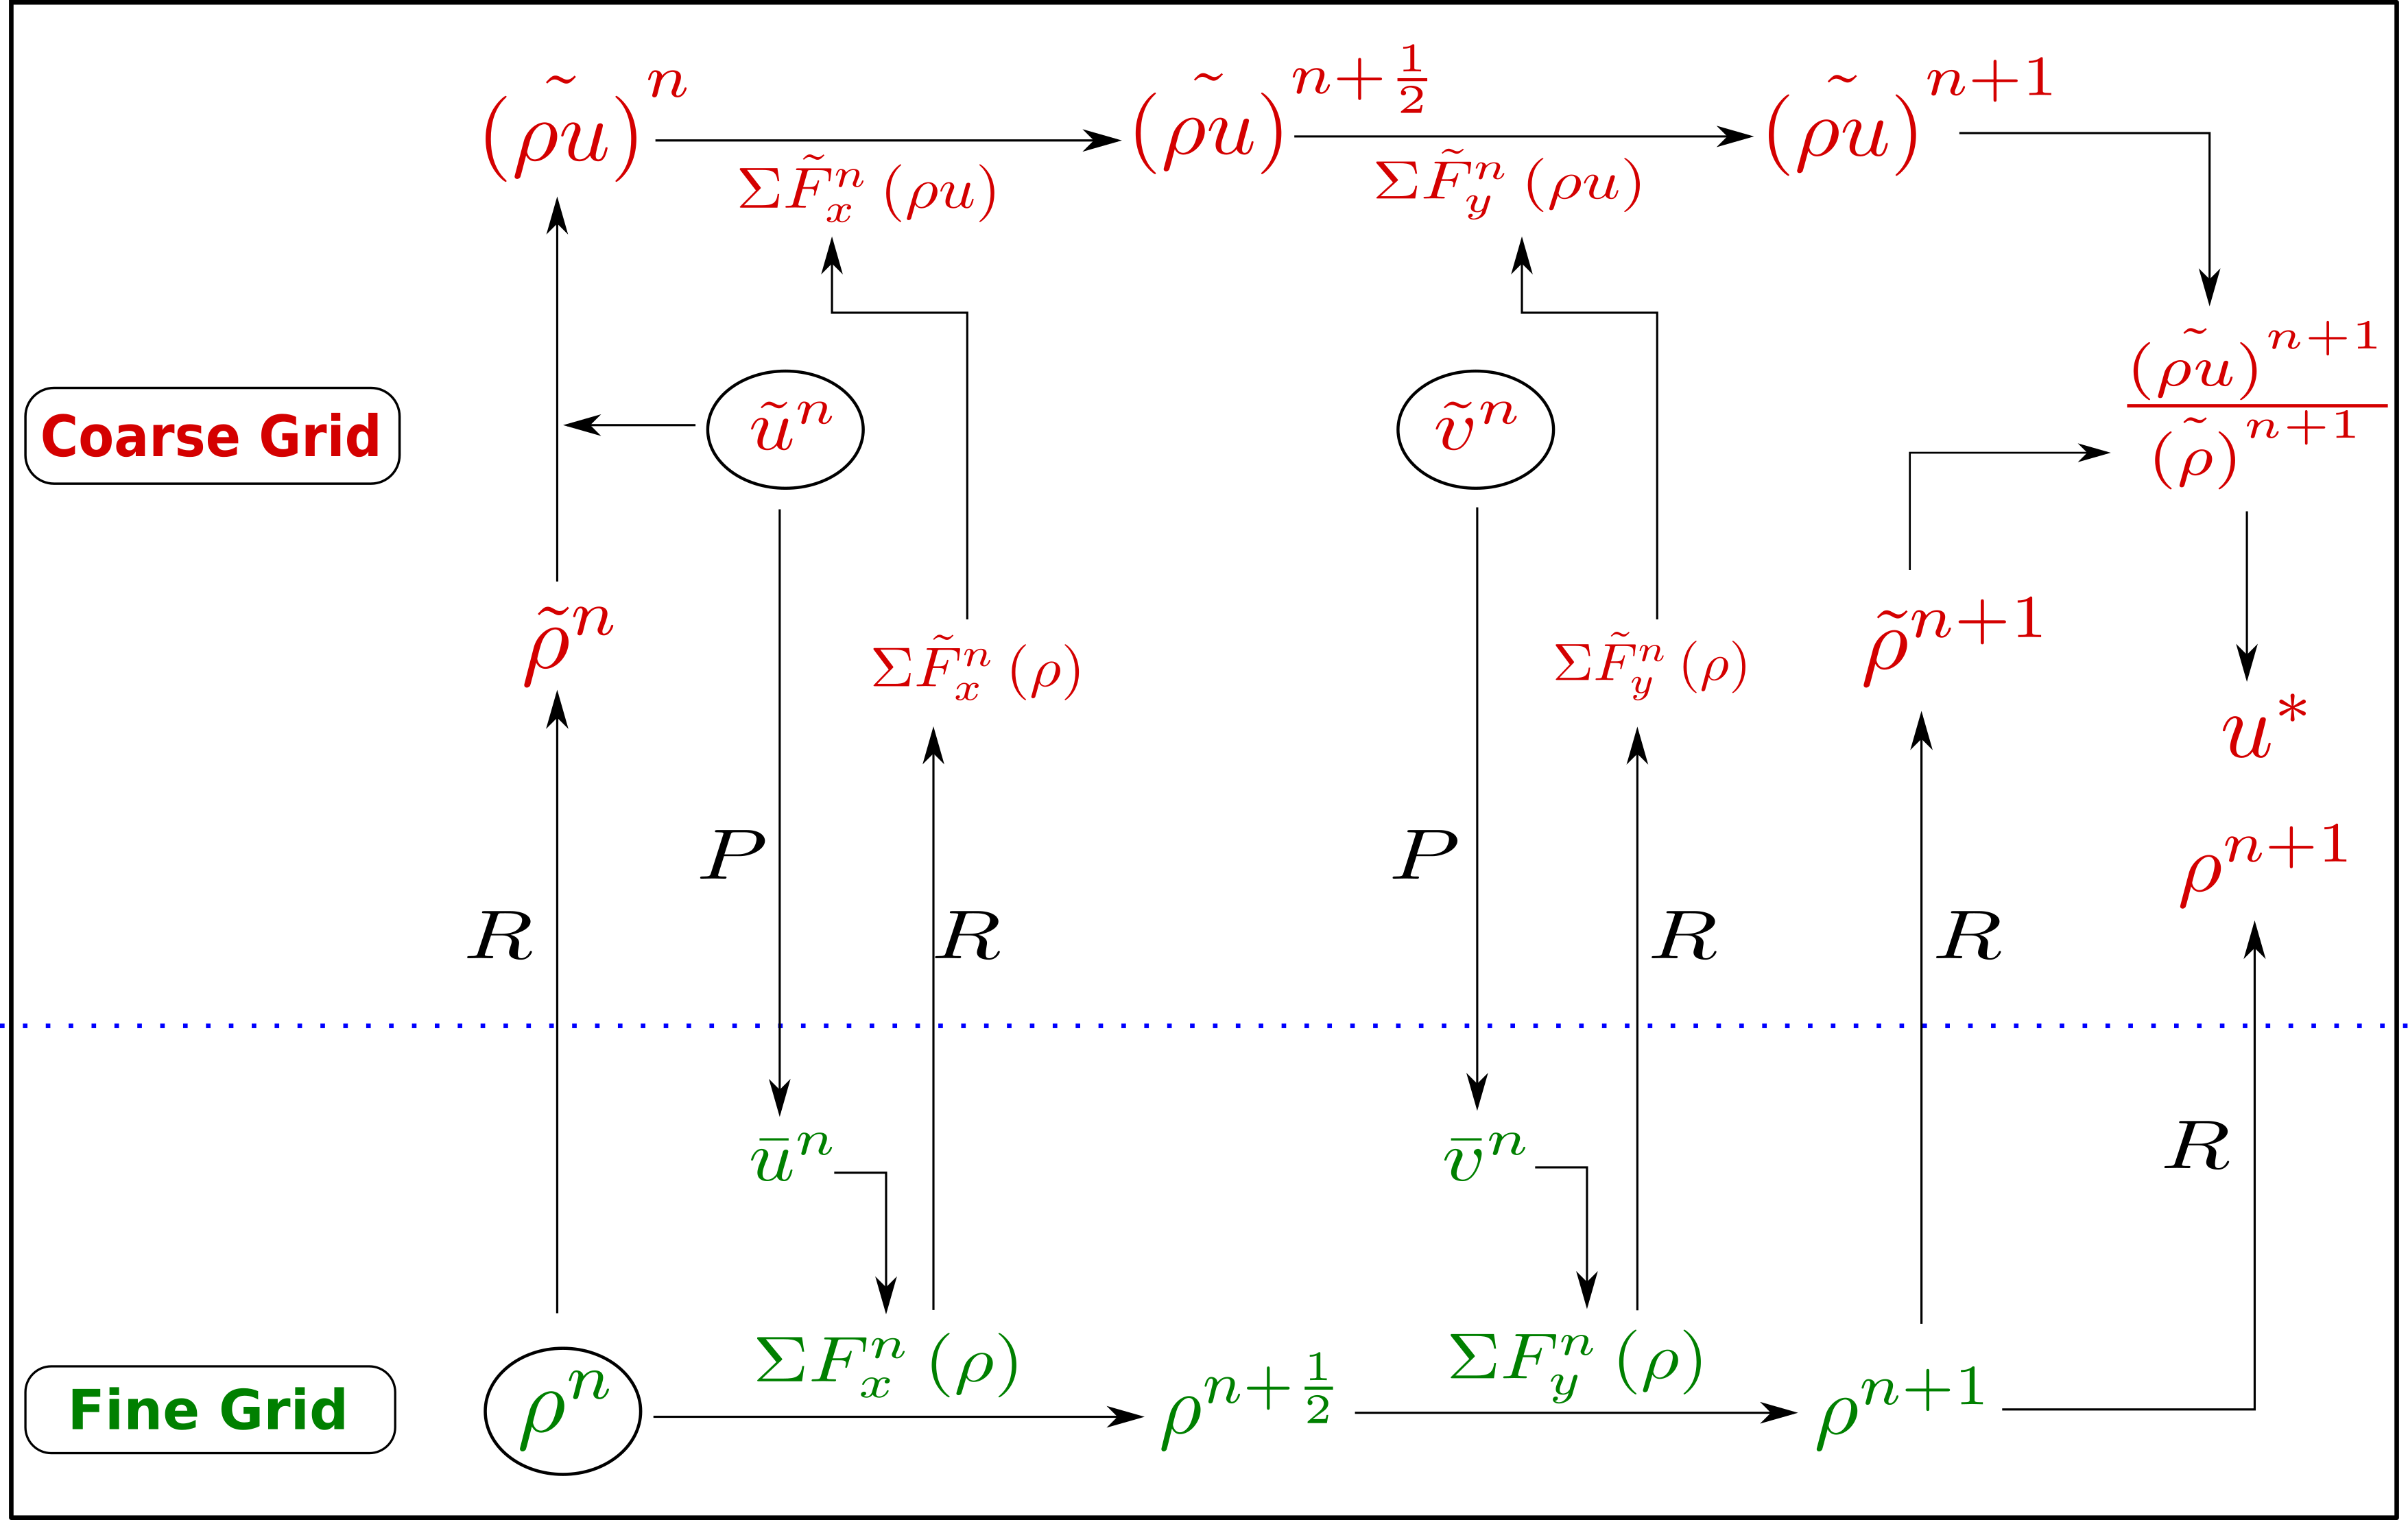
\includegraphics[width = \textwidth]{plots/momcons_sagar.png}
\caption{A bird's eye view of the \textit{sub-grid} method,
highlighting the operations performed at each time step. 
and additionally ensures conservation of momentum.
For sake of clarity, present a 2D case for the
density on the grid $i,j$ and horizontal velocity $\tilde{u}$ 
on the staggered grid $i+1/2,j$.
The variables in red are all defined on the coarse level, 
and those in green are at the sub-grid level. 
The operators $R$ and $P$ denote the restriction and 
prolongation operations respectively.
The 'tilde' on top of the variables (e.g. $\tilde{\rho}^{n} $) are 
used to convery that the variables are centered on the  
staggered control volumes at the coarse grid level, whereas the 'bar' 
on top conveys that the variables are staggered with respect to the sub-grid. 
The starting variables are enclosed in elliptical borders, 
and the variables at the end of the direction-split 
integrations are $u^{*}$ and $\rho^{n+1}$,
where $u^{*}$ is subsequently fed into the RHS of the Poisson problem. 
}
\label{momcons_sagar}
\end{figure}



\begin{enumerate}

\item Interface reconstruction at time $t_n$, at the sub-grid level,
	using data $c^{n}$.
        
	\marginnote{$q=1,2$ is the component index, 
	e.g $\rho_1$ in $\Omega_{i+1/2,j}$ for the 
	horizontal momentum component $\rho_1 u_1$.
	}

\item Restriction of the sub-grid volume fraction in order     
	to compute the ``shifted'' fraction fields $C^{n}_q$ and $\rho^{n}_q$
	in the staggered control volumes.

\item Computation of all momentum components $(\rho_q u_q)^{n}$
	at $t_n$.
	\marginnote{ The fluxes of momentum are derived from those of mass
		using the relation \eqref{frou} ,
		which in turn are obtained via restriction operations applied 
		to the sub-grid volume fraction fluxes. 
		}

\item Advection of the sub-grid volume fraction $c^n$ along one coordinate direction, 
	say $x$ direction, to obtain $c^{n + \frac{1}{2}}$ , using the Weymouth-Yue explicit advection method.  
	
\item Advection of all momentum components along the $x$ direction, 
	in sync with the sub-grid VOF advection, 
	using \eqref{sumfmom2} to obtain the updated momentum components
		$(\rho_q u_q)^{n + \frac{1}{2}}$ after the first substep.

\item Restriction of the sub-grid field $c^{n + \frac{1}{2}}$ as shown in Fig. \ref{restrict}
	, in order to compute the ``shifted'' density field $\rho^{n + \frac{1}{2}}_q$ on the staggered volumes. 

\item Extraction of the provisional velocity components 
	\sidenote{These provisional velocities are required
		to compute the ``advected'' velocities using 
		the non-linear flux limiters, as described in \eqref{advect-ed-ing-2}.}
		$u_q^{n + \frac{1}{2}}$ after the first substep, 
		i.e. $u_q^{n + \frac{1}{2}} = (\rho_q u_q)^{n + \frac{1}{2}}/\rho_q^{n + \frac{1}{2}}$.

\item The above operations are repeated for the different momentum components,
	in sync with the direction-split advection of the sub-grid volume fraction
	along the remaining direction. 
\sidenote{At each time step, the sequence $x, y$ is permuted, in order to avoid 
any systematic biases in error propagation.}
Finally, we obtain $u_q^{*} = (\rho_q u_q)^{n + 1}/\rho_q^{n + 1}$ on the staggered grid.

\item In parallel, the updated centered volume fraction field $C^{n+1}$ is obtained  
	at the coase grid level, by applying the restriction operator 
	on the updated sub-grid volume fraction $c^{n+1}$. 

\end{enumerate}

The resulting method not only maintains discrete consistency between
mass and momentum transport on the staggered grid, but also ensures that
the transport of momentum is consistent in 3D.
The other time-split terms in equation (\ref{mom_update}) 
that arise from the source term discretizations, as well 
as the terms in the projection step \eqref{ufinal} are solved in 
a standard non-conservative way, and are briefly covered in what follows. 
The density on the faces of the central cells 
are estimated using the restriction operations
\marginnote{
Generally, the face-centered density field 
is estimated using a simple average i.e. $\rho_{i+1/2,j,k} = (\rho_{i,j,k} + \rho_{i+1,j,k})/2$. 
}
described previously, with these densities appearing 
via the $ 1 / \rho_q $ pre-factor in front of all
the terms in the momentum transport (e.g surface tension, viscous diffusion) 
that are discretized in a non-conservative manner. 
Additionally, the sub-grid volume fraction
can be used to get better estimates of the curvature field, which
itself is defined on the staggered control volumes. 
At the time of writing, two different approaches are being 
developed and tested in order to get more accurate curvature fields. 
The detailed descriptions of the methods used in our 
numerical platforms to deal with surface tension,
viscosity and body forces have already been carried 
out in \cite{paris, basilisk, popinet2009accurate}, 
therefore we briefly touch upon certain aspects of the 
operators in question, in particular, 
their interaction with the volume fraction field.

\subsection*{Surface Tension}
We use the Continuum Surface Force method (CSF) as our model for surface tension, 
coupled with height functions for curvature computation. 
The height functions used in our implementation were first introduced in \cite{popinet2009accurate}
, subsequently tested, revised and improved in \cite{bornia2011properties,owkes2015mesh}. 
In general, the height functions are used to compute the curvature field based 
on second-order finite differences applied to the heights. 
Although, in regions of poor interfacial resolution 
\sidenote{These are regions where the local radius of curvature is comparable to the grid size, in fact 
for certain cases the height functions perform poorly even for regions resolved by 10-20 grid points.}, 
the method reverts to certain fallbacks, one of which is curve fitting instead of height functions.  
The resulting curvature field is coupled with a well-balanced discretization with
respect to the discrete pressure gradient, with the same discretization 
stencil applied to the volumetric (body) force term as well. 


\subsection*{Viscous Diffusion}
We use second-order spatial discretizations of the viscous stresses, using centered differences
\sidenote{The exact implementation differs slightly between `Basilisk' and `PARIS Simulator'.}. 
The (variable) dynamic viscosity is computed based on the  
volume fraction field via weighted arithmetic or harmonic averaging (equations \ref{mu_chi}). 
The temporal treatment of the viscous term can be either in explicit or semi-implicit fashion,  
, but in the context of the present study we will be sticking exclusively with the explicit version.     


\subsection*{Pressure-Poisson Projection}

The velocity field is evolved using a classical time-splitting projection method 
as described in the seminal work of Chorin \cite{chorin1969convergence}, 
which involves predicting an `intermediate' velocity field $\boldsymbol{u}^{*}$ 
as given by equation \ref{mom_update}, followed by a correction step as follows        

\begin{align}
\boldsymbol{u}^{n+1} = \boldsymbol{u}^{*} - \frac{\tau}{\rho^{n+1}}\nabla^{h}p^{n+1}
\label{ufinal}
\end{align}

The discrete pressure field required to correct the intermediate velocity 
is determined by imposing the conservation of mass, which in our incompressible 
framework reduces to necessitating the resulting velocity field to be divergence-free (solenoidal)  

\begin{align}
\nabla^{h}\cdot\boldsymbol{u}^{n+1} = 0
\label{div}
\end{align}

Thus, combining equations \ref{ufinal} and \ref{div}, 
we are left with a variable coefficient Poisson equation for the pressure :  

\begin{align}
\nabla^{h}\cdot\left(\frac{\tau}{\rho^{n+1}}\nabla^{h}p^{n+1}\right) = \nabla^{h}\cdot \boldsymbol{u}^{*} 
	\label{poisson}
\end{align}

The Poisson solver used in `PARIS Simulator' to invert the elliptic operator 
appearing in eqn. \ref{poisson} is a red-black 
Gauss-Seidel (GS) solver with overrelaxation \sidecite{briggs1987}. 
There is also has an in-house implementation of a multigrid solver 
for structured grids with $2^{n}$ number of points per direction, 
utilizing a fully parallelized V-Cycle scheme \cite{briggs1987}. 
Relaxation operations are applied starting from the finest to the coarsest first, 
and then from the coarsest to the finest, with the number of relaxation operations 
being a user-adjustable parameter. Having a native multigrid solver allows 
for an efficient solution of the Poisson equation without the necessity
of having external libraries/pre-conditioners (e.g. HYPRE) installed on the system.
When it comes to `Basilisk', an atypical multigrid solver is implemented using 
a ``half'' V-cycle in order to deal with the spatial inhomogeity of the grid size
arising due to adaptive mesh refinement. 
For more details regarding the differences between the multigrid solver of `Basilisk'
and the classical implementation of a multigrid, one can refer to \sidecite{popinet_gerris}.


The whole set of operations described up to this point, 
constitutes a temporal integration scheme of the first-order, which can be expressed as 

\begin{align}
\left(C^{n+1},\boldsymbol{u}^{n+1}\right) = L_{1}\left( C^{n},\boldsymbol{u}^{n} \right)
\end{align}

where $L_{1}$ is the operator consisting of all the steps described 
so far, applied to the primary fields $C$ and $\boldsymbol{u}$. 
Therefore, a second-order time integration can easily be 
computed by using $L_{1}$ to get a first prediction    

\begin{align}
\left(C^{**},\boldsymbol{u}^{**}\right) = L_{1}\left( C^{n},\boldsymbol{u}^{n} \right)
\end{align}

The superscript $**$ refers to our first order prediction of the primary variables. 
Therefore, the second-order estimate can be obtained via averaging   

\begin{align}
\left(C^{n+1},\boldsymbol{u}^{n+1}\right) = \frac{1}{2}\left[ \left(C^{**},\boldsymbol{u}^{**} \right) + L_{1}\left( C^{**},\boldsymbol{u}^{**} \right) \right]
\end{align}

%---------------------------------------------------------------


In the following chapter, we shall take a look at some performance 
aspects of these mass-momentum consistent methods,
using both quantitative and qualitative comparisons. 


%\setchapterpreamble[u]{\margintoc}
\chapter{Methodology}
\labch{method}

%---------------------------------------------------------------
% overview of chapter 
In this chapter, we describe the basic numerical methodology behind our models 
concerning the dynamics of immiscible liquid-gas interfacial flows, at the incompressible and isothermal limits. 
These implementations are developed on the platforms 'PARIS Simulator' \cite{paris} and 
'Basilisk' \cite{popinetbasilisk}, with considerable overlap between the two platforms in terms 
of the treatment of the interface capturing schemes, transport of conserved quantities and surface tension models.
\sidenote{The principle difference between 'PARIS Simulator' and 'Basilisk' is the ability to resolve the conservation
laws on dynamically adaptive meshes in the case of 'Basilisk', whereas 'PARIS Simulator' only deals with regular Cartesian meshes.}
The numerical implementations are based on finite volume discretizations on uniform or dynamically refined Cartesian grids , utilizing
state of the art methods in interfacial reconstruction coupled with geometric
transport of the corresponding fluxes, curvature computation and surface tension modeling. For more detailed
descriptions of the general capabilities of 'PARIS Simulator’ and 'Basilisk', we refer the reader to the previously cited references. 


\section{Governing Equations}

We use the one-fluid formulation for our system of governing equations, thus solving 
the incompressible Navier-Stokes equations throughout the whole domain including regions 
of variable density and viscosity, which itself depend on the explicit 
location of the interface separating the two fluids.
In the absence of mass tranfer, the velocity field is continuous across
the interface at the incompressible limit, with the interface evolving according to the local velocity vector.  
Generally, we have a choice regarding how to model the convective operator
of the incompressible Navier-Stokes equations. There is a well established corpus of 
numerical methods tailored specifically to deal with non-conservative 
\sidenote{also referred to as the strong form, necessitating certain orders of smoothness of the primitive variable} form of the convective 
operator that appear in transport equations of mass and momentum 
\sidenote{These methods are descendants of the class of numerical schemes used to solve hyperbolic partial differential equations.}
, which perform quite well in the context of single phase flows.
However, in interfacial flows we often deal with discontinuities that arise as a consequence
of the contrast in material properties between the two fluids. Therefore, even though the velocity field
remains continuous throughout the domain, the otherwise smooth density (mass) and momentum fields 
contain sharp jumps (discontinuities) localized at the interfacial position.     





% in incompressible flows, the velocity field is continuous in the absence of mass transfer across the interface 

\begin{align} 
	\frac{\partial \rho}{\partial t} + \nabla\cdot \left(\rho\boldsymbol{u}\right) &= 0 \nonumber \\
	\frac{\partial}{\partial t} \left(\rho\boldsymbol{u}\right) + \nabla\left(\rho\boldsymbol{u}\otimes\boldsymbol{u}\right)  &= -\nabla p + \nabla \cdot \left(2 \mu \boldsymbol{D}\right) + \sigma \kappa \delta_{s}\boldsymbol{n} + \rho \boldsymbol{g}
\label{nseqn}
\end{align}


with $\rho$ and $\mu$ being the density and dynamical viscosity respectively, and therefore are the physical quantities which are discontinuous across the interface. The volumetric sources are modeled by the acceleration $g$, and the deformation rate tensor $\boldsymbol{D}$ used to model the viscous stresses is defined as:  

\begin{align}
	\boldsymbol{D} = \frac{1}{2}\left[\nabla \boldsymbol{u} + \nabla \boldsymbol{u}^{T}\right]  
\end{align}


The term $\sigma \kappa \delta_{s}\boldsymbol{n}$ represents the surface tension forces in the framework of the continuum surface-force model (CSF). The normal vector to the interface is $\boldsymbol{n}$, with $\sigma$ being the coefficient of surface tension and $\kappa$ the local interfacial curvature. The operator $\delta_{s}$ is the Dirac delta function, the numerical approximation of which, allows us to map the interfacial surface force distribution onto their volumetric equivalents for our Cartesian control volumes. In the case of incompressible flows, advection of mass is equivalent to the advection of volume, and within the Volume-of-Fluid framework the Eulerian transport of the interface allows us to track the temporal evolution of the volume fractions of the two fluids. Thus, the transport of the interface governs the temporal evolution of the volume fraction field as: 

% explain continuous nature of velocity field in limit of no mass transfer 

% explain one-fluid model NS eqns

\paragraph{Description of Operators}
\blindtext


% also explain how diffusion and capillary force operators are computed, briefly


\paragraph{Evolution of phase-characteristic function}
\blindtext


% evolution of marker function - marker functiona approximated by LS, VOF etc

\paragraph{Material Properties}
\blindtext

% possibility of harmonic mean in play 

%---------------------------------------------------------------

\section{Interface Tracking}

\paragraph{Volume-of-Fluid : PLIC Methodology}
\blindtext

\paragraph{Flux Computation : CIAM , WY}
\blindtext

%---------------------------------------------------------------

\section{Time Marching}

\paragraph{Spatio-Temporal Discretization}
\blindtext

\paragraph{Pressure-Projection Algorithm}
\blindtext



%\setchapterpreamble[u]{\margintoc}
\chapter{Consistent Mass-Momentum Transport}
\labch{momcons}

% intro : PARIS Simulator, necessity due to large density-ratios ? 


% ----------------------------------------------------------------------------------------------------------------------

\section{General Principles}

%intro : what do you mean by consistent transport?  


\subsection*{Major Iterations in Literature}

% literature review 
% modified comparison charts with CAF paper added

\subsection*{Our Approach}

% approach of reconstruction on staggered cells, geometric flux computations , well-balanced surface force model 


% ----------------------------------------------------------------------------------------------------------------------


\section{Consistent Transport : Basic Expressions}

% intro : advection of a generic conserved quantity 

\subsection*{Advection of Density}

% VOF - rho consistency with compression term etc

\subsection*{Advection of Momentum}

% model of computing consistent mass-momentum fluxes

\subsection*{Advected Velocity}

% computation of slope limiters with diagram, distinction in bulk and interfacial regions


% ----------------------------------------------------------------------------------------------------------------------


\section{Staggered Reconstructions}

% intro : staggered configuration of primary variables, control volumes for staggered advection 

\subsection*{Shifted Fractions Method}

% algorithm, flow chart , how to reconstruct on shifted grid, lack of conservation 

\subsection*{Sub-Grid Method}

% algorithm, flow chart, prolongation and restriction operations, consistent + conservative 

\subsection*{Source Terms}

% 1/rho terms in ST , reconstructing curvatures from sub-grid information etc 

\setchapterpreamble[u]{\margintoc}
\chapter{Numerical Benchmarks}
\labch{numbench}

In the upcoming sections, we demonstrate the robustness and accuracy of our class of mass-momentum consistent numerical methods when applied to challenging flow configurations involving marked density contrasts, primarily in comparison with the version of our method which does not maintain consistency between the mass and momentum advection. Most of the standard tests that exist in the current literature concerning numerical methods to tackle liquid-gas flows such as the decay of spurious currents in static and moving droplets, viscous damping of capillary waves etc., are carried out in the absence of any density jump (or viscosity jump) across the interface separating the fluids. In this chapter, we shall take a closer look in detail at the behavior of our methods when dealing with difficulties that arise due to the non-linear coupling between interfacial deformation/propagation, capillary and viscous forces, especially in the regime where the material properties across the interface are separated by orders of magnitude, particularly in which the flow features in question are poorly resolved. 

In order to assess the performance of the different methods, we shall use an easier nomenclature to describe the different methods, which are as follows : 

\begin{itemize}
	\item \textbf{STD} : The standard method which does not maintain consistency between mass and momentum transport. 
	\item \textbf{MSHIFT} : The method that ensures consistency between mass and momentum transport, 
		but is not exactly momentum conservative. 
		It is based on the \textit{shifted fractions} strategy, 
		as detailed in the previous chapter. 
	\item \textbf{MSUB} : The method that ensures both consistency between mass and momentum transport, as well as ensuring exactly conservative transport. It uses the \textit{sub-grid} strategy as discussed in the preceding chapter. 
\end{itemize}

%------------------------------------------ STATIC DROP ---------------------------------------------

\section{Static Droplet}
\labsec{static}

A popular numerical benchmark in the existing literature relevant to surface tension dominated flows is the case of a spherical droplet of the denser fluid immersed in a quiescent surrounding medium of the lighter fluid. In the hydrostatic limit of the Navier-Stokes equations, the droplet should stay in equilibrium, with a curvature induced pressure jump across the interface corresponding to Laplace's equilibrium. In practice however, numerically reproducing such a trivial equilibrium condition is not as straightforward, as there exists a slight difference between the initial numerical interface and the exact analytical shape of the sphere, thereby resulting in the generation of the well documented '\textit{spurious}' or '\textit{parasitic}' currents of varying intensity in the velocity field \sidecite{lafaurie1994modelling, harvie2006analysis, popinet1999front}. A lot or progress has been made since in the context of \textit{well-balanced} surface tension formulations, that ensure consistency between the numerical stencils used for the discretization of the pressure gradient and the Heaviside approximation ($n \delta_{s}$) that projects the the surface force distribution onto the control volumes \cite{francois2006balanced,popinet2009accurate}. A significant contribution to the interpretation of these parasitic currents within the well-balanced framework was made by Popinet \cite{popinet2009accurate} which demonstrated that given sufficient time (of the order of viscous dissipation time-scales), a well-balanced method will relax to the '\textit{numerical}' equilibrium shape through the damping of the 'physically consistent' numerical capillary waves, therefore allowing us to recover the exact (to machine precision) Laplace equilibrium condition.

\subsection*{Setup}

% insert figure  

\begin{figure}[h!]
    \centering
    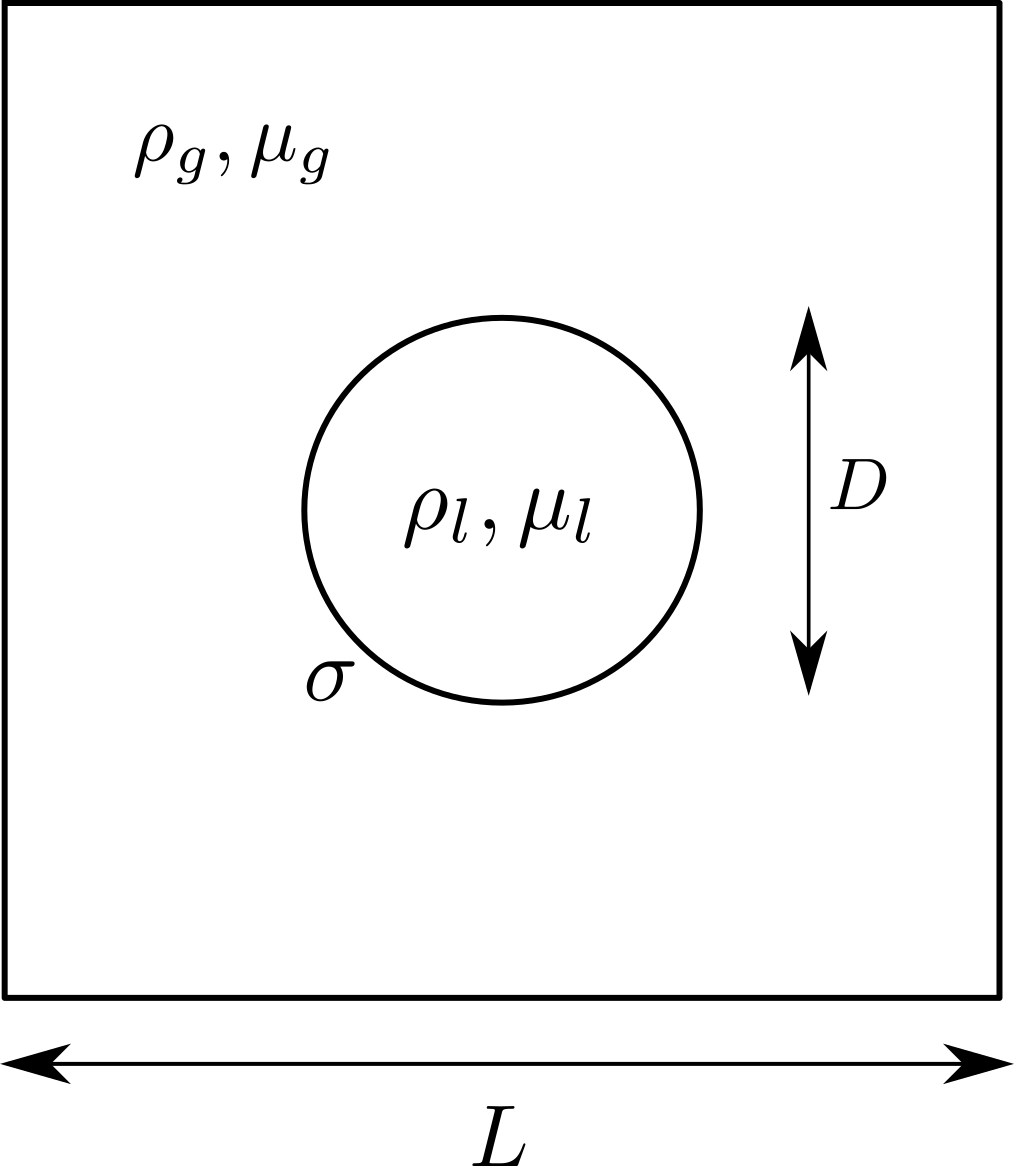
\includegraphics[width = 1.0\textwidth]{plots/static_drop/config.png}
    \caption{Schematic of the static droplet of dense fluid surrounded by a quiescent medium of lighter fluid. A $40 \times 40$ grid is employed to spatially discretize the domain.}
    \label{static_conf}
\end{figure}

% difference in our setup in terms of high-density ratios
The key difference in our implementation of this classic test case from that of Popinet \sidecite{popinet2009accurate} is that we consider the effect of density contrast across the interface separating the fluids. As we have previously discussed, a sharp density jump across the interface may have an amplification effect on the numerical errors incurred as a result of interfacial reconstructions, curvature estimation and various other truncations, thereby rendering the method unstable. We demonstrate that in our framework of mass consistent momentum transport coupled with a well-balanced surface tension discretization, density-ratios as large as $1000:1$ can be simulated without loss of numerical stability, in conjuction with the ability to recover the exact numerical equilibrium through the dissipation of spurious currents within relevant time-scales \sidenote{The viscous time-scale corresponding to the droplet length-scale is the most commonly used in literature.}.

% specification of numerical problem setup, domain, densities and viscosities
We consider a circular droplet of size $D$  placed at the centre of a square domain of side $L$. The densities of the heavier and lighter phases are $\rho_l$ and $\rho_g$ respectively, likewise for the viscosities $\mu_l$ and $\mu_g$, and $\sigma$ being the surface tension coefficient (fig. \ref{static_conf}). The ratio of the droplet size to the box is chosen as $D/L = 0.4$, coupled with a numerical resolution of $D/\Delta x= 16$ (where $\Delta x$ is the grid size). As for boundary conditions, we use symmetry conditions on all sides of the square domain.

% specification of problem parameters and adimensional numbers 
The problem incorporates two natural time-scales, the capillary oscillation scale and the viscous dissipation scale, which are defined below :

\begin{align}
        T_\sigma = \left(\frac{\rho_l D^3}{\sigma}\right)^{1/2} \quad , \quad T_\mu = \frac{\rho_l D^2}{\mu_l}
\label{ts}
\end{align}

The ratio of these time-scales give us -

\begin{align}
	\frac{T_\mu}{T_\sigma} = \sqrt{\rho_l \sigma D}/\mu_l = \sqrt{\textrm{La}}
\end{align}

where $\textrm{La}$ is the Laplace number based upon the heavier fluid. In the present study, we introduce the density-ratio $\rho_l/\rho_g$ as another important parameter. In order to rescale our 'parasitic' velocity field, we define a velocity scale based on capillary oscillations as -

\begin{align}
        U_\sigma = \sqrt{\sigma/\rho_l D}
\end{align}

Additionally, the time-step in our numerical simulation must be smaller than the oscillation period corresponding to the grid wavenumber (fastest capillary wave with a time period $\sim \left( \rho_l \Delta x^3 / \sigma  \right)^{1/2} $ ) as a stability criterion \sidenote{Similar criteria are defined on the basis of the viscous and advection operators as well, with the smallest amongst the three selecting the numerical time-step}, as our surface tension model is explicit in time. For the scope of the present study, we shall not consider any viscosity contrast between the two fluids while varying the density-ratio, therefore $\mu_l/\mu_g = 1$ for all the cases under study.


\subsection*{Decay of Spurious Currents}

In figures \ref{decay_nonmc} to \ref{decay_sagar}, we illustrate the decay of the root-mean-square of the spurious currents as a function of time, in the case of four different density-ratios, with three different Laplace numbers for each ratio. The first figure (\ref{decay_nonmc}) refers to simulations carried out without consistency between the momentum-mass transport (\textbf{STD}), the second (\ref{decay_daniel}) corresponds to that of the consistent but not conservative method (\textbf{MSHIFT}), and final one (\ref{decay_sagar}) refers to that of the consistent and conservative method (\textbf{MSUB}). The time is rescaled by the viscous dissipation scale, and the spurious currents by the capillary velocity scale. We have two main observations, the rapid decay of the rescaled spurious currents for all combinations of density-ratios and Laplace numbers within approximately $0.2 T_{\mu}$, and the slower re-growth of the currents in question for combinations of non-unity density-ratios and large Laplace numbers, in all simulations except those carried out with \textbf{MSUB}. With method \textbf{MSUB}, the decayed currents keep hovering around levels of machine precision for remainder of time. Although there is a re-growth of the currents using the consistent method (\textbf{MSHIFT}) after $0.2 T_{\mu}$, the behavior is not quite alarming as the rate of this re-growth is quite low. Therefore, out of all the methods tested, the consistent and conservative method (\textbf{MSUB}) does seem to demonstrate the desired performance, especially when it comes to combinations of large density contrasts coupled with large Laplace numbers.   


\begin{figure}[h!]
    \centering
    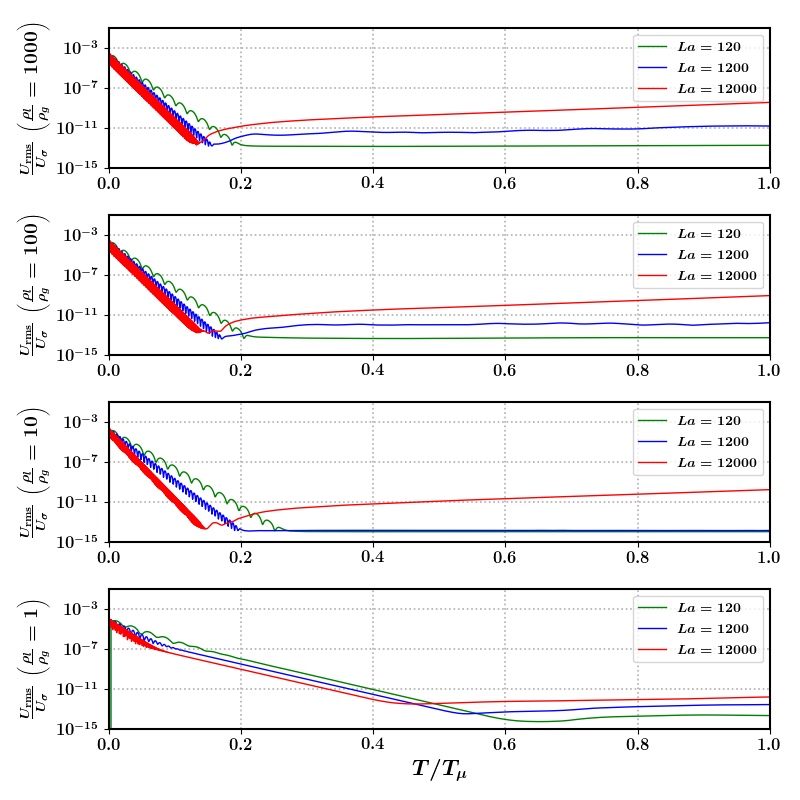
\includegraphics[]{plots/static_drop/decay_nonmc.png}
	\caption{\textbf{STD} Decay of normalized spurious currents as a function of viscous dissipation time-scales for different density-ratios and Laplace numbers. The currents seem to initially decay quickly for all higher density-ratios, and relax to the numerical equilibrium curvature even within $0.2 \cdot T_\mu$. For combinations of large $\rho_l / \rho_g$ and large $\textrm{La}$, the spurious currents seem to grow back to an order of magnitude ($10^{-8}$) which is quite far from that of machine precision ($10^{-14}$).}   
    \label{decay_nonmc}
\end{figure}

\begin{figure}[h!]
    \centering
    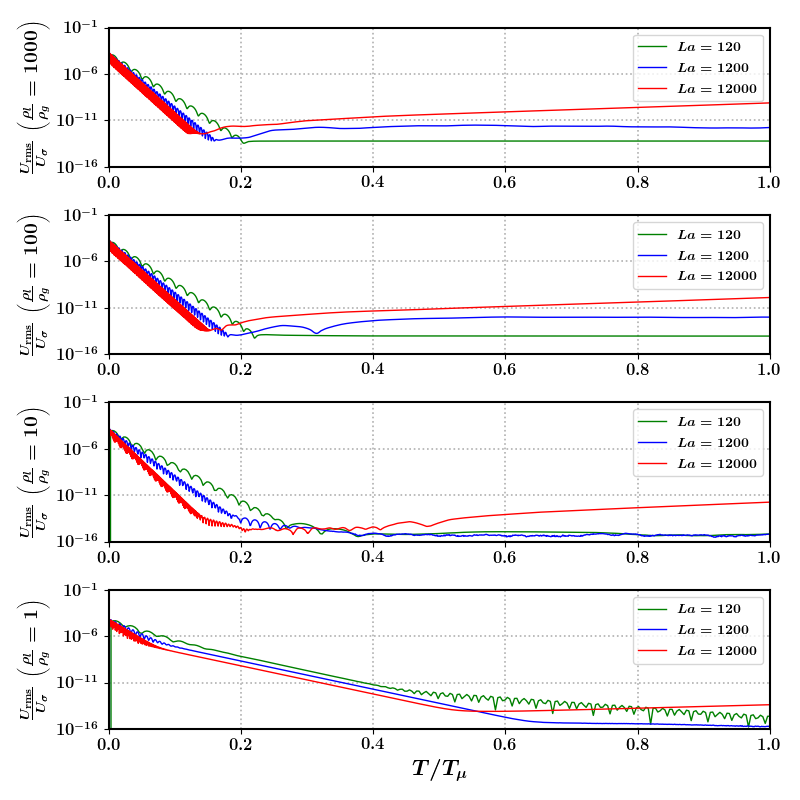
\includegraphics[]{plots/static_drop/decay_daniel.png}
	\caption{\textbf{MSHIFT} Decay of normalized spurious currents as a function of viscous dissipation time-scales for different density-ratios and Laplace numbers. The currents seem to initially decay quickly for all higher density-ratios, and relax to the numerical equilibrium curvature even within $0.2 \cdot T_\mu$. For combinations of large $\rho_l / \rho_g$ and large $\textrm{La}$, the spurious currents seem to grow back to an order of magnitude ($10^{-8}$) which is quite far from that of machine precision ($10^{-14}$). No considerable improvement is observed with respect to \textbf{STD}. }   
    \label{decay_daniel}
\end{figure}

\begin{figure}[h!]
    \centering
    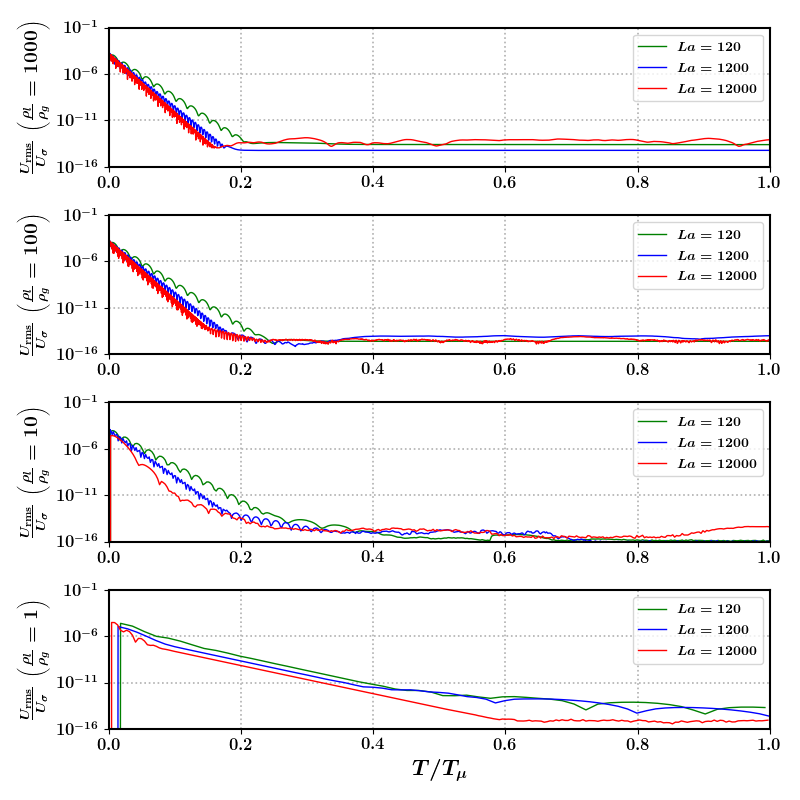
\includegraphics[]{plots/static_drop/decay_sagar.png}
	\caption{\textbf{MSUB} Decay of normalized spurious currents as a function of viscous dissipation time-scales for different density-ratios and Laplace numbers. The currents seem to decay very quickly in the case of higher density-ratios, and relax to the numerical equilibrium curvature even within $0.2 \cdot T_\mu$. For all combinations of $\rho_l / \rho_g$ and $\textrm{La}$ numbers, the decayed spurious currents are not observed to grow back as in the cases of \textbf{STD} and \textbf{MSHIFT}, and hover around values close to machine precision ($10^{-14}$).}   
    \label{decay_sagar}
\end{figure}



\subsection*{Spatial Convergence}

Once the solution relaxes to a numerical equilibrium curvature (spurious currents are approximately at the order of machine precision), there still exists a difference between the numerical curvature and the exact analytical curvature corresponding to the spherical (circular) shape. We use the definitions of the shape errors as introduced in the seminal work of Popinet \cite{popinet2009accurate} to assess the convergence of our class of methods to the exact (analytical) curvature as we increase spatial resolution. The norms are defined as follows :      

\begin{align}
	L_2 = \sqrt{\frac{\sum_i \left(C_i - C_i^\text{exact} \right)^2}{\sum_i}} \quad , \quad L_\infty = \text{max}_i \left( | C_i - C_i^\text{exact} | \right)
  \label{shape_err_norms}
\end{align}

where $C_i$ is the volume fraction of a cell after the solution has relaxed to the numerical equilibrium curvature, and $C_i^\text{exact}$ is the volume fraction corresponding to the exact circular shape which was initialized at the start of the simulation.  

Fig. \ref{static_drop_conv} demonstrates the behavior of the shape errors defined in eqn. \ref{shape_err_norms} for the case of the most stringent parameter combination ( $\rho_l / \rho_g = 1000 $ , $\textrm{La} = 12000$ ) as a function of the droplet resolution. As one can clearly observe, all the methods tested display a roughly second-order convergence in space for both the error norms. In terms of the $L_2$ norm, the consistent and conservative method (\textbf{MSUB}) does indeed achieve smaller errors as compared to both \textbf{STD} and \textbf{MSHIFT} for all spatial resolutions. As a minor remark, there is not much to discern in terms of shape error when it comes to comparing the performances of the consistent (\textbf{MSHIFT}) method with the non-consistent one (\textbf{STD}). 

\begin{figure}[h!]
    \centering
    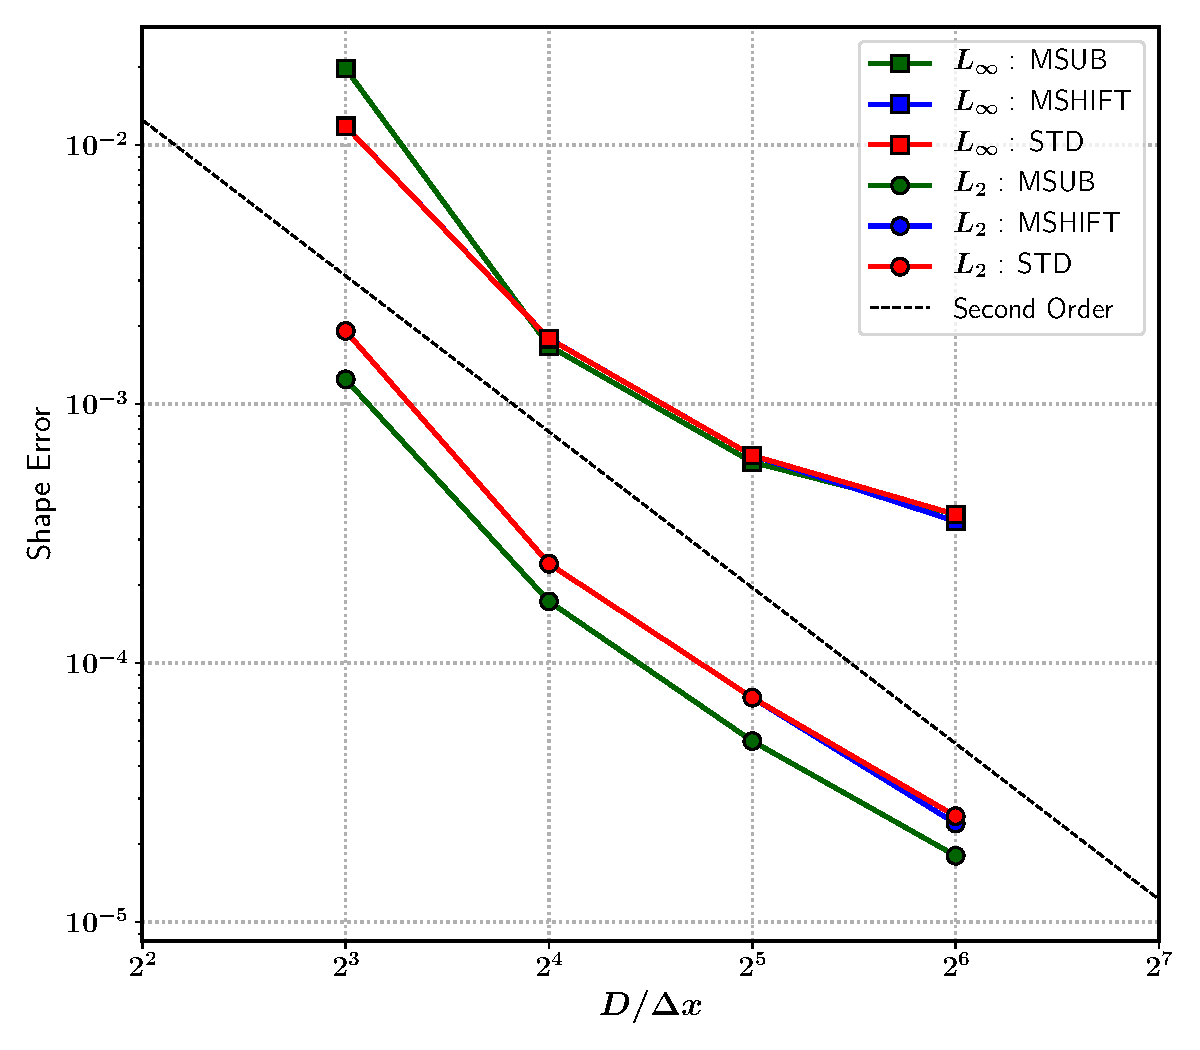
\includegraphics[width = 1.0\textwidth]{plots/static_drop/convergence.pdf}
	\caption{Second-order spatial convergence for the spurious current error norms corresponding to the most stringent parameter combination ($\rho_l/\rho_g = 1000$ , $\textrm{La} = 12000$) . Both of the norms ($L_\infty$ and $L_2$) seem to demonstrate a roughly second order rate of spatial convergence with each of the methods tested. However, \textbf{MSUB} has a marginally lower $L_2$ error compared to both \textbf{STD} and \textbf{MSHIFT} for all resolutions tested. There is negligible difference observed in the shape errors between \textbf{STD} and \textbf{MSHIFT} in both of the norm definitions.}   
    \label{static_drop_conv}
\end{figure}


%------------------------------------------ MOVING DROP ---------------------------------------------

\section{Moving Droplet}

An incisive numerical setup that enables us to evaluate the accuracy of the coupling between interfacial propagation and surface tension discretization was first proposed by Popinet \cite{popinet2009accurate}, and subsequently employed in the comparative study of Abadie et al. \sidecite{abadie2015combined}. The manner in which this test differs from that of the static droplet is the addition of a uniform background velocity field, therefore serving as a better representation of droplets in complex surface tension dominated flows where they might be advected by the mean flow. In terms of the Laplace equilibrium, the hydrostatic solution is still valid in the frame of reference of the moving droplet. The point at which the solution in the moving reference frame diverges from that of the static droplet (\ref{sec:static}) is through the continuous injection of noise at the scale of the grid size. This 'numerical' noise emanates from the perturbations to the curvature estimates, which are in turn induced by the interfacial reconstructions carried out to propagate the interface (temporal integration) . These fluctuating errors act as source terms for the momentum, thereby transforming the problem into that of viscous dissipation in the presence of continuous forcing (in the reference frame of the moving drop).

\subsection*{Setup}

\begin{figure}[h!]
    \centering
    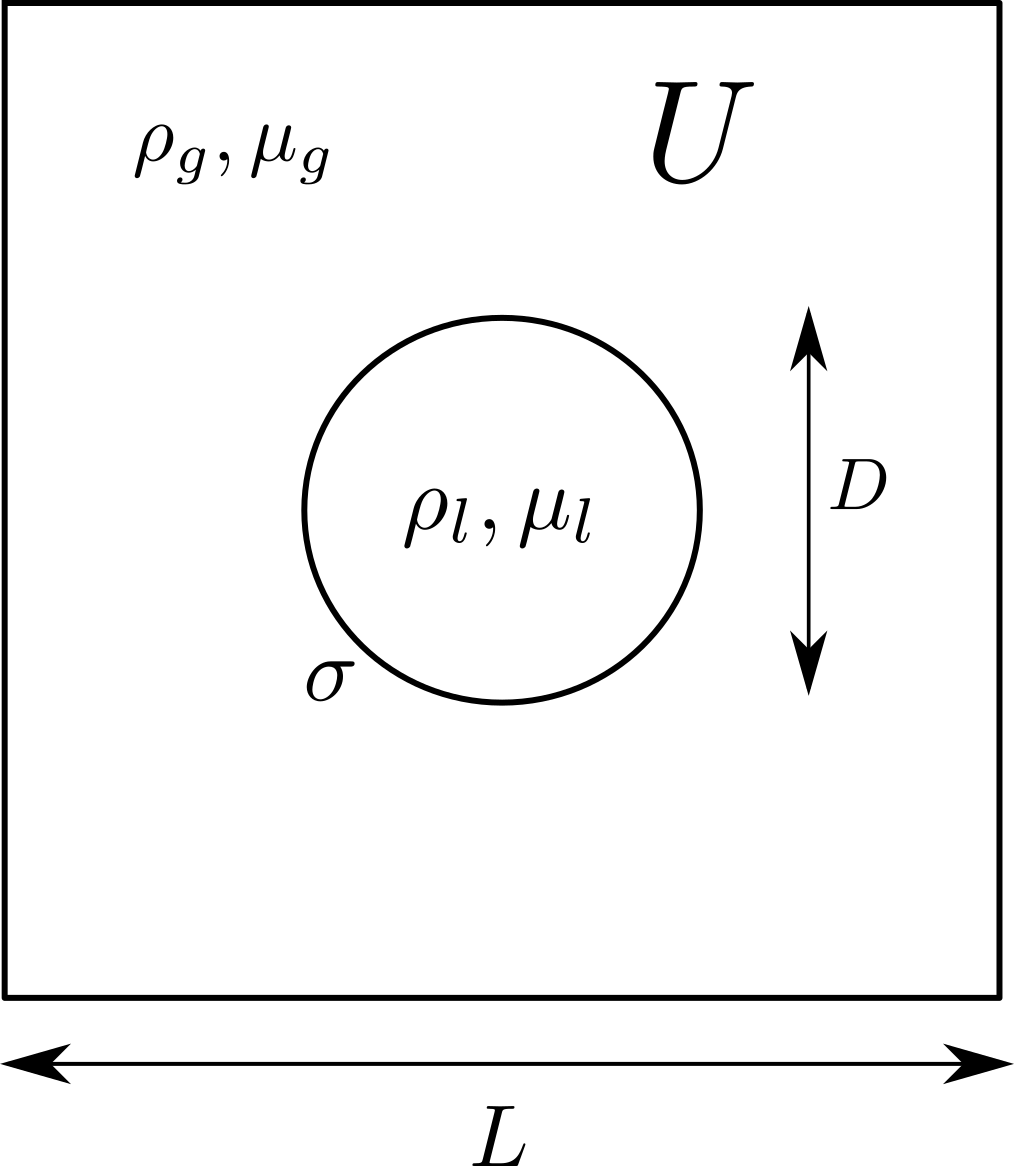
\includegraphics[width = 1.0\textwidth]{plots/droplet_advect/config.png}
    \caption{Schematic of the droplet of dense fluid advected in a surrounding medium of lighter fluid. A $50 \times 50$ grid is employed to spatially discretize the domain, which is spatially periodic in the direction of droplet advection.}
    \label{moving_conf}
\end{figure}

In the present study, we evaluate our class of methods using the advection of a droplet in a spatially periodic domain using an identical setup as \cite{popinet2009accurate}, but with the important difference of including sharp density jumps across the interface as well as using lower spatial resolutions. As previously discussed (\ref{sec:static}), large density contrasts tend to amplify the fluctuations induced by the myriad numerical approximations (interface reconstruction, curvature estimation etc) involved in the algorithm.

We consider a circular droplet of diameter $D$ placed at the centre of a square domain of side $L$. The densities of the heavier and lighter phases are $\rho_l$ and $\rho_g$ respectively, likewise for the viscosities $\mu_l$ and $\mu_g$, and $\sigma$ being the surface tension coefficient (fig. \ref{moving_conf}). A uniform velocity field $\boldsymbol{U}$ is initialized on the entire domain (only a horizontal component). The ratio of the droplet size to the box is $D/L = 0.4$, with $D/\Delta x= 20$ ($\Delta x$ being the grid size. \sidenote{In Popinet \cite{popinet2009accurate}, a resolution of $D / \Delta x = 25.6$ corresponding to a grid of $64 \times 64$ is used } ). As for boundary conditions, we use symmetry conditions on the top and bottom sides, and periodic boundary conditions on the horizontal direction (along which advection by $U$ takes place). We characterize by problem by introducing the following adimensional parameters (based on the heavier fluid) :

\begin{align}
	\textrm{La} = \frac{\rho_l \sigma D}{\mu_l^2} \quad , \quad \textrm{We} = \frac{\rho_l U^2 D}{\sigma}
\end{align}

In addition to the capillary and viscous time-scales for the static case (eqns. \ref{ts}), we have an additional scale defined as :

\begin{align}
	T_{u} = D/U
\end{align}

which is the time-scale of advection. In our subsequent analysis, we shall use $T_u$ and $U$ as the time and velocity scales, repectively.

\subsection*{Evolution of Spurious Currents}

\begin{figure}[h!]
    \centering
    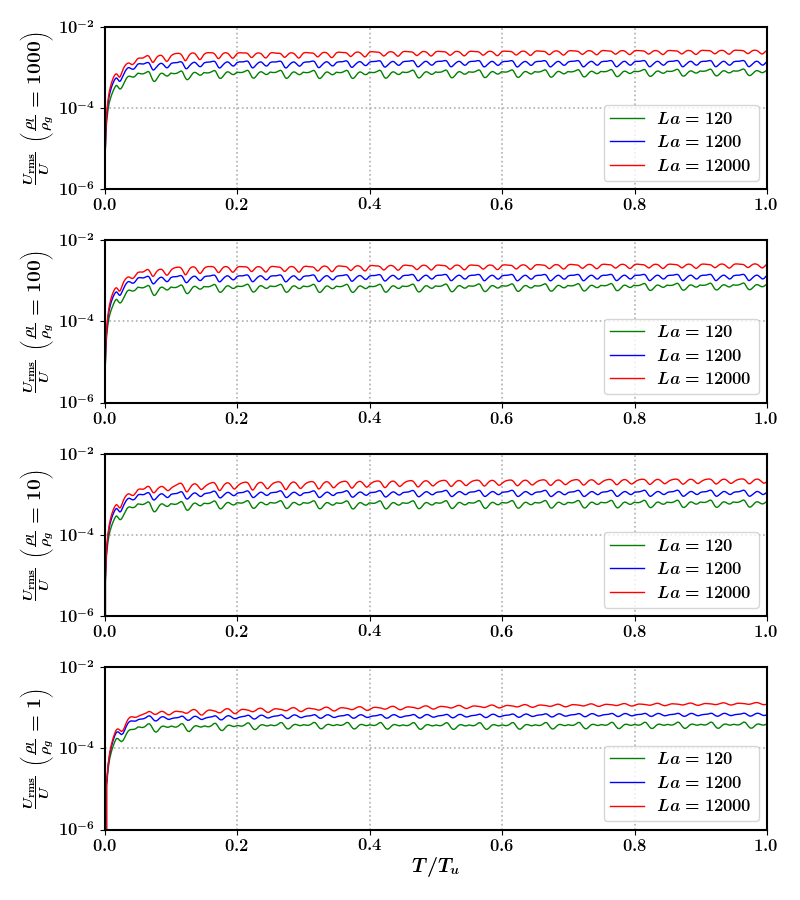
\includegraphics[]{plots/droplet_advect/evo_nonmc.png}
	\caption{\textbf{STD} Time evolution of normalized spurious currents as a function of advection time-scales ($T_u$) for different combinations of density-ratio and Laplace numbers. The currents seem to hover around $10^{-3}$, with a larger Laplace number corresponding to a higher error for all density-ratios. $\textrm{We} = 0.4$ for all the cases presented.}   
    \label{evo_nonmc}
\end{figure}

\begin{figure}[h!]
    \centering
    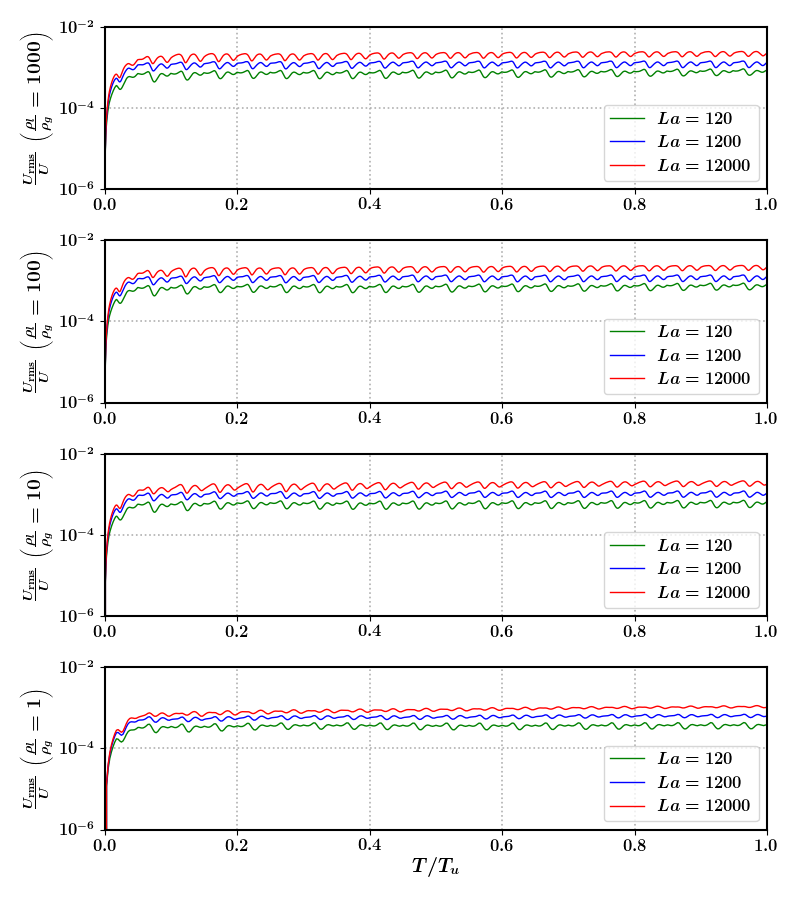
\includegraphics[]{plots/droplet_advect/evo_daniel.png}
	\caption{\textbf{MSHIFT} Time evolution of normalized spurious currents as a function of advection time-scales ($T_u$) for different combinations of density-ratio and Laplace numbers. There seems to be no appreciable difference from the evolution seen in the case of \textbf{STD} (fig. \ref{evo_nonmc}). The currents seem to hover around $10^{-3}$, with a larger Laplace number corresponding to a higher error for all density-ratios. $\textrm{We} = 0.4$ for all the cases presented.}   
    \label{evo_daniel}
\end{figure}

\begin{figure}[h!]
    \centering
    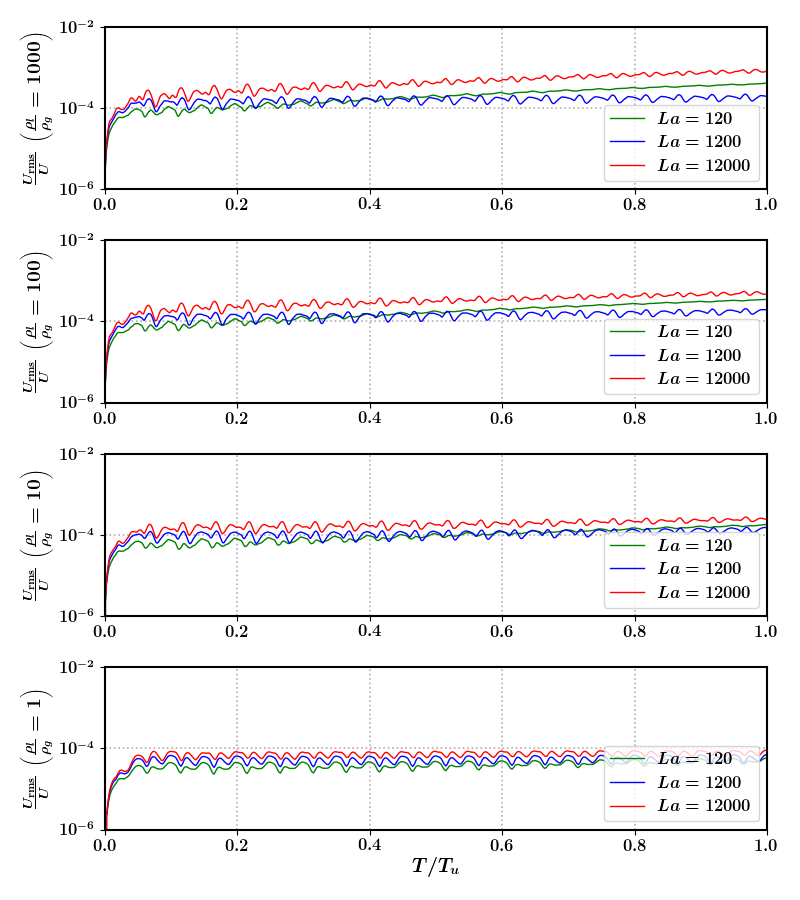
\includegraphics[]{plots/droplet_advect/evo_sagar.png}
	\caption{\textbf{MSUB} Time evolution of normalized spurious currents as a function of advection time-scales ($T_u$) for different combinations of density-ratio and Laplace numbers. In terms of the errors observed in \textbf{STD} and \textbf{MSHIFT}, we observe a decrease of roughly one order of magnitude. Although an upward trend is observed for large Laplace numbers, the growth rate is quite low. The currents seem to hover slightly above $10^{-4}$, with larger Laplace numbers corresponding to larger errors for all density-ratios. $\textrm{We} = 0.4$ for all the cases presented.}   
    \label{evo_sagar}
\end{figure}

Figures \ref{evo_nonmc} to \ref{evo_sagar} depict the evolution of the root-mean-square (RMS) error of the velocity field in the moving frame of reference, as a function of different Laplace numbers, spanning over density ratios separated by orders of magnitude. The first figure (\ref{evo_nonmc}) refers to simulations carried out without consistency between the momentum-mass transport (\textbf{STD}), the second (\ref{evo_daniel}) corresponds to that of the consistent but not conservative method (\textbf{MSHIFT}), and final one (\ref{evo_sagar}) refers to that of the consistent and conservative method (\textbf{MSUB}). We again have a couple of important observations, the first being that spurious currents do not decay to machine precision as in the static droplet case for all of the combinations and methods tested, instead they oscillate around a mean value of the order of $(0.1-0.01)\% $ of the constant field $U$. The second observation is regarding the significantly smaller error (almost by one order of magnitude) in the case of the consistent and conservative method (\textbf{MSUB}) when compared to that of \textbf{STD} and \textbf{MSHIFT}. As a minor remark, in case of large Laplace numbers, the \textbf{MSUB} method displays a slight upward trend in the error evolution, which is not the case in either \textbf{STD} or \textbf{MSHIFT}. This is not too worrisome as the growth is over a time-scale much larger than $T_u$, with the oscillations corresponding to a time-scale of the order $U/\Delta x$. All of the plots in figures \ref{evo_nonmc} to \ref{evo_sagar} correspond to $\textrm{We} = 0.4$, alongside an additional simplification of equal viscosities across the interface i.e $\mu_l/\mu_g = 1$ .

As evindenced by the persistence of these spurious currents due to the addition of grid-level noise emanating from interfacial reconstructions, further advancements should be made with respect to the combined performace of the interfacial transport, curvature computation and the surface tension model. Nonetheless, all the methods tested do seem to be quite numerically stable when dealing with the high density-ratios, and are not subject to rapid uncontrollable amplifications of the interfacial perturbations even for high Laplace numbers.

\subsection*{Spatial Convergence}

In order to evaluate the performance of our class of methods at different resolutions, we define the errors as the maximum values of the norms $L_\infty$ and $L_2$ of the rescaled field $U_{rms}/U$ over time ($5$ times $T_u$). In fig. \ref{moving_drop_conv}, we show the scaling of the error as a function of spatial resolution for the most stringent case of $\rho_l/\rho_g = 1000 $ , $\textrm{La} = 12000$, for each of our different methods. As similarly observed in section \ref{sec:static}, in terms of both $L_\infty$ and $L_2$ norms, there is no appreciable difference in the behaviors of \textbf{STD} and \textbf{MSHIFT}. For \textbf{MSUB}, we do observe significantly lower maximum errors compared to other two methods, but at a cost of slightly less than first-order convergence. The overall convergence behavior of the class of methods we have tested seems to be consistent with earlier studies of Popinet \cite{popinet2009accurate} and others \sidenote{In existing literature, convergence rates have only been studied in case of equal density fluids across the interface} .  

\begin{figure}[h!]
    \centering
    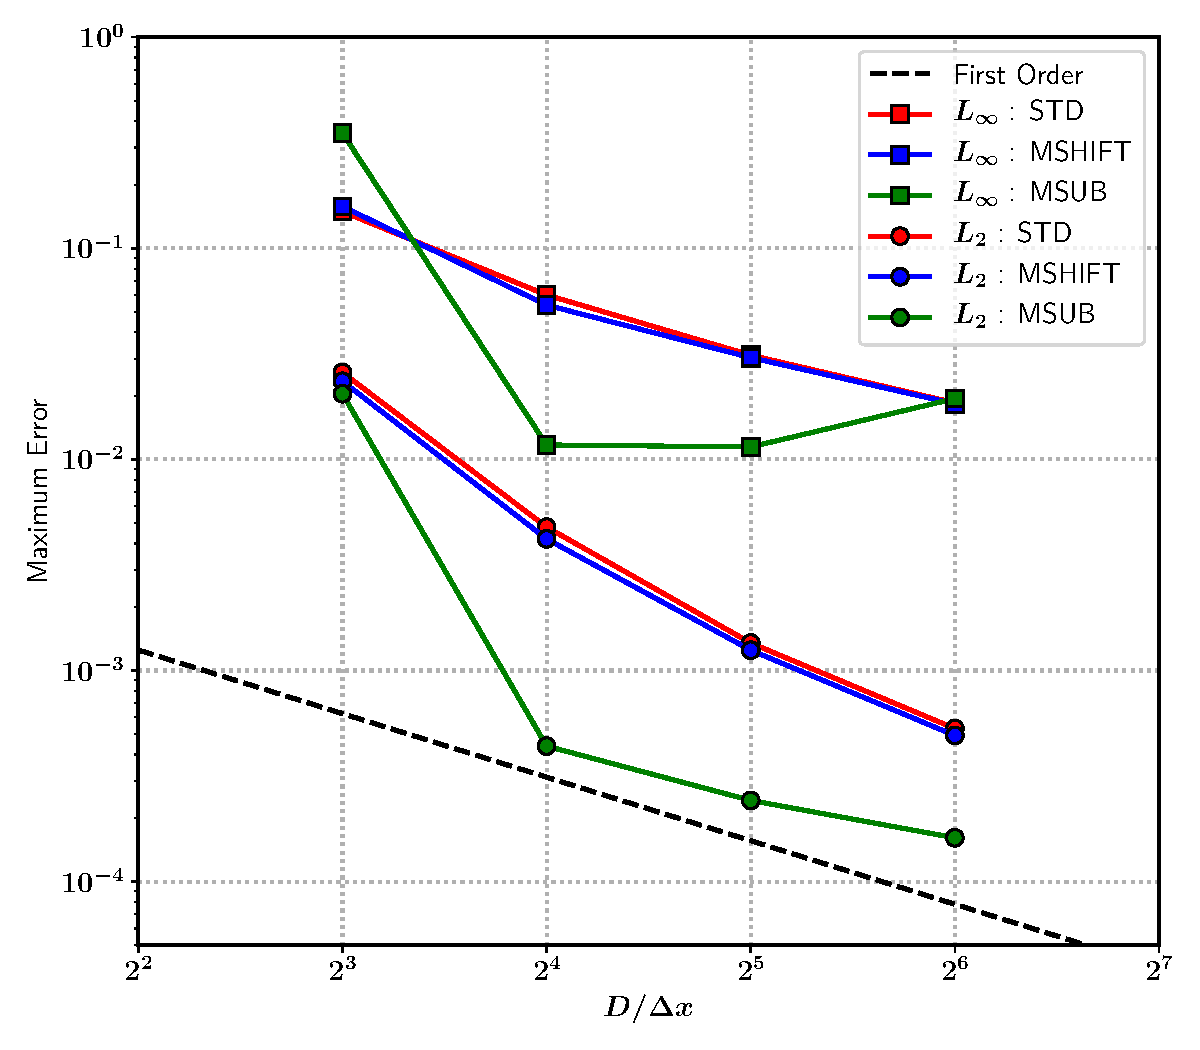
\includegraphics[width = 1.0\textwidth]{plots/droplet_advect/convergence.pdf}
	\caption{First-order (approximately) spatial convergence of the maximum of the spurious current error norms in the frame of reference of the moving droplet, for the most stringent parameter combination ($\rho_l/\rho_g = 1000 $ , $\textrm{La} = 12000$, $\textrm{We} = 0.4$). Methods \textbf{STD} and \textbf{MSHIFT} display similar convergence properties, whereas \textbf{MSUB} leads to significantly lower errors even though it doesn't quite follow the first-order convergence rate. }   
    \label{moving_drop_conv}
\end{figure}

\subsection*{Error Dependence : Laplace \& Weber numbers}

As the final point of inquiry into the performance of our class of methods, figures \ref{web} and \ref{lap} demonstrate the influence of the Laplace and Weber numbers on the behavior of the maximum error norm, carried out for the largest density-ratio ($\rho_l/\rho_g = 1000$). We present results obtained using the consistent and conservative method (\textbf{MSUB}), for a resolution corresponding to $D / \Delta x = 25.6$. As we can observe, the error (both $L_\infty$ and $L_2$) scales as $\textrm{We}^{-1/3}$ over 4 orders of magnitude, which is different from the $\textrm{We}^{-1/2}$ scaling observed by Popinet \cite{popinet2009accurate} \sidenote{ Although Popinet \cite{popinet2009accurate} had equal densities ($\rho_l/\rho_g = 1$) }. In terms of Laplace numbers, the errors scale as $\textrm{La}^{1/6}$ over two orders of magnitude, which is the same as that observed in \cite{popinet2009accurate} (for equal densities).

\begin{figure}
    \centering
    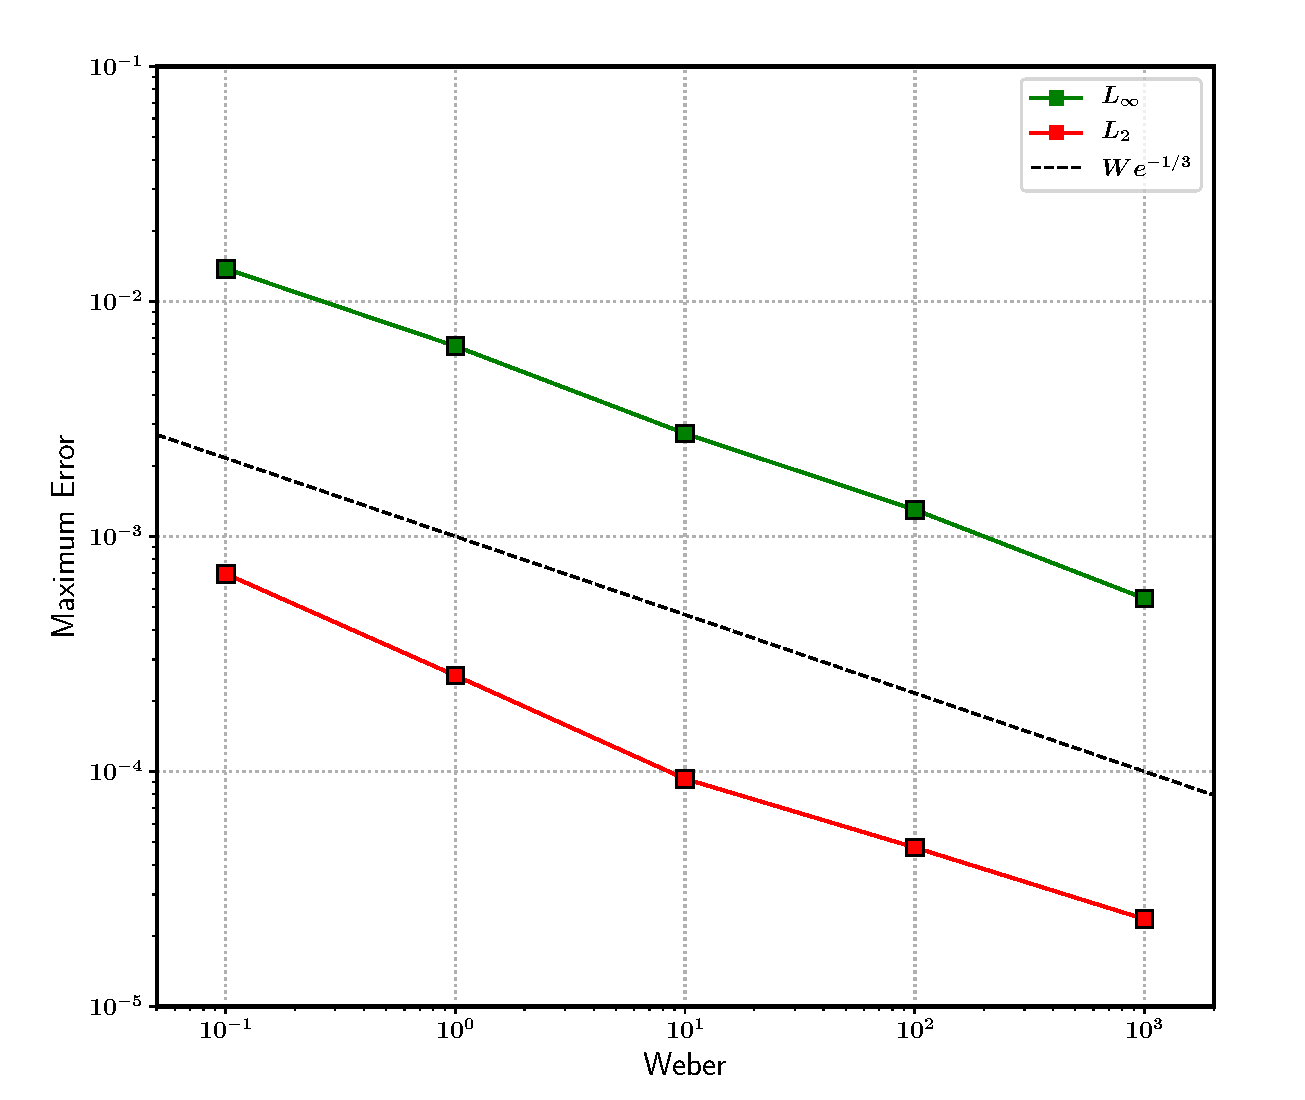
\includegraphics[width = 1.0\textwidth]{plots/droplet_advect/webers.pdf}
	\caption{ Scaling of the maximum error norm as a function of Weber ($\textrm{La} = 12000$, $\rho_l / \rho_g = 1000$). }
    \label{web}
\end{figure}

\begin{figure}
    \centering
    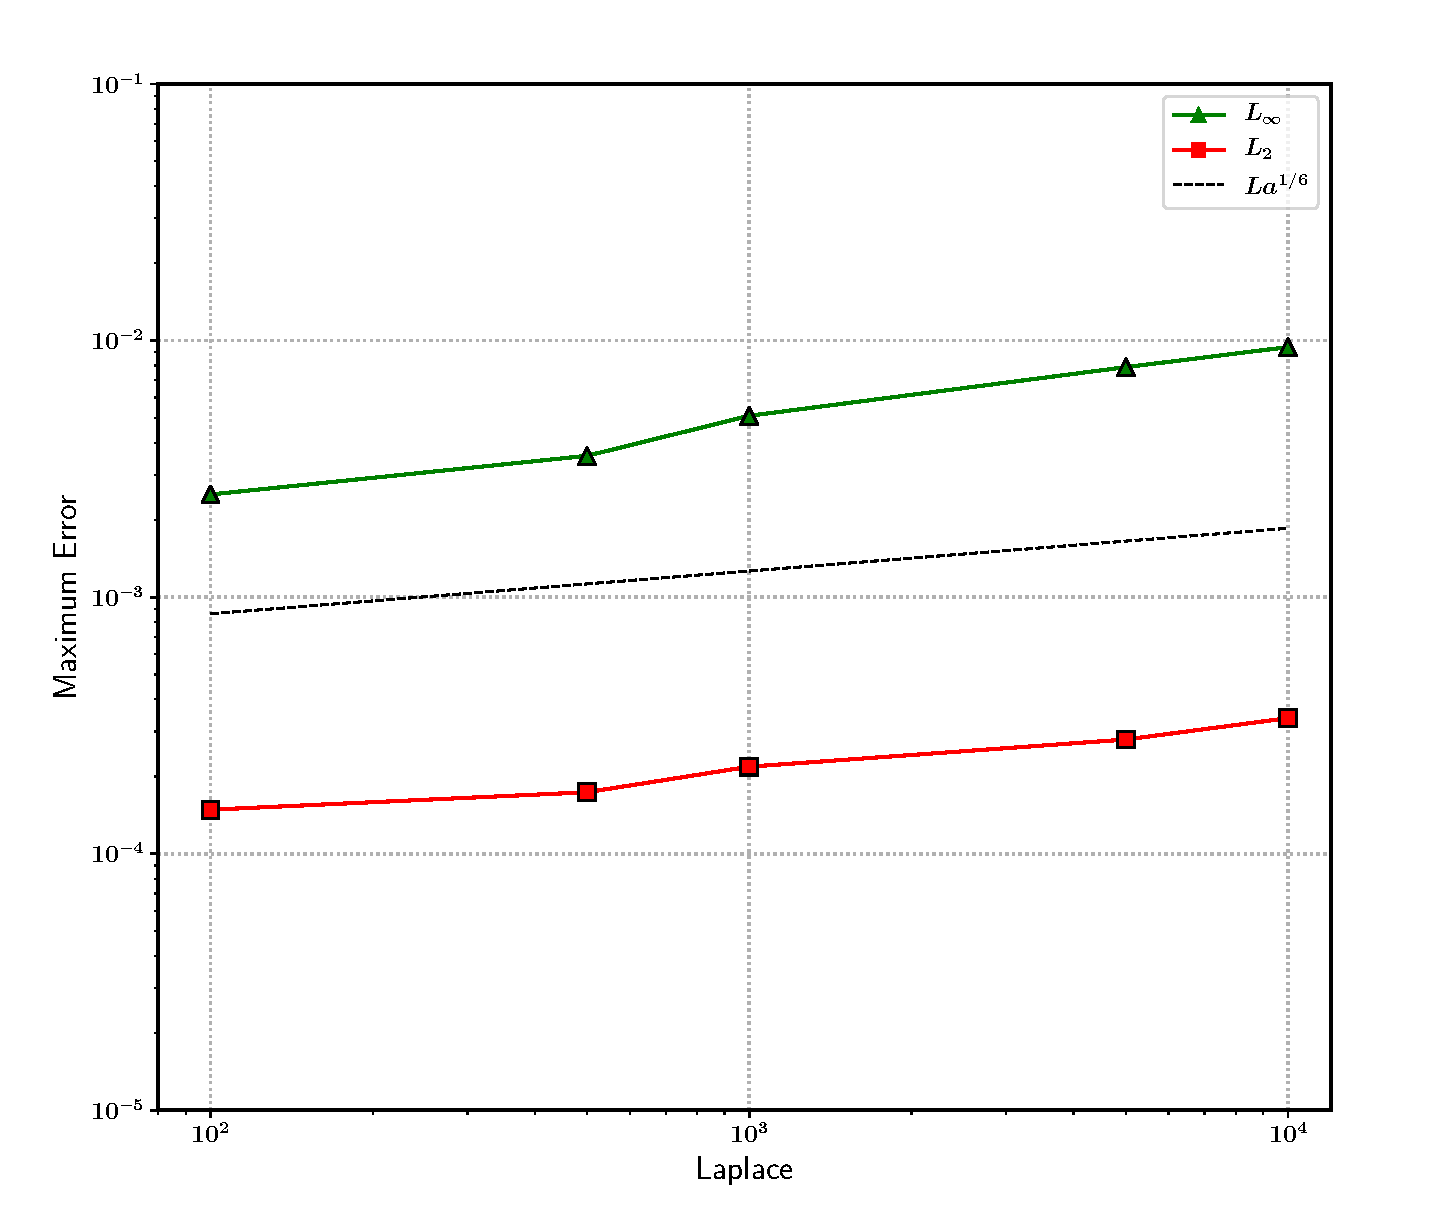
\includegraphics[width = 1.0\textwidth]{plots/droplet_advect/laplaces.pdf}
	\caption{ Scaling of the maximum error norm as a function of Laplace ($\textrm{We} = 0.4$, $\rho_l / \rho_g = 1000$). }
    \label{lap}
\end{figure}



%------------------------------------------ CAPILLARY WAVE ---------------------------------------------

\section{Capillary Wave}
One of the fundamental features of immiscible multiphase flows involving interfaces are the presense and propagation of capillary waves. Therefore, a robust and accurate numerical method should not only be able to adequately resolve, but also accurately emulate the spatio-temporal evolution of such surface tension induced oscillations. A brief outline on the state-of-the-art numerical implementations of capillary waves (and surface tension models in general) existing in current literature is provided by Popinet in the comprehensive review \sidecite{popinet2018numerical}.

\subsection*{Setup}

\begin{figure}[h!]
    \centering
    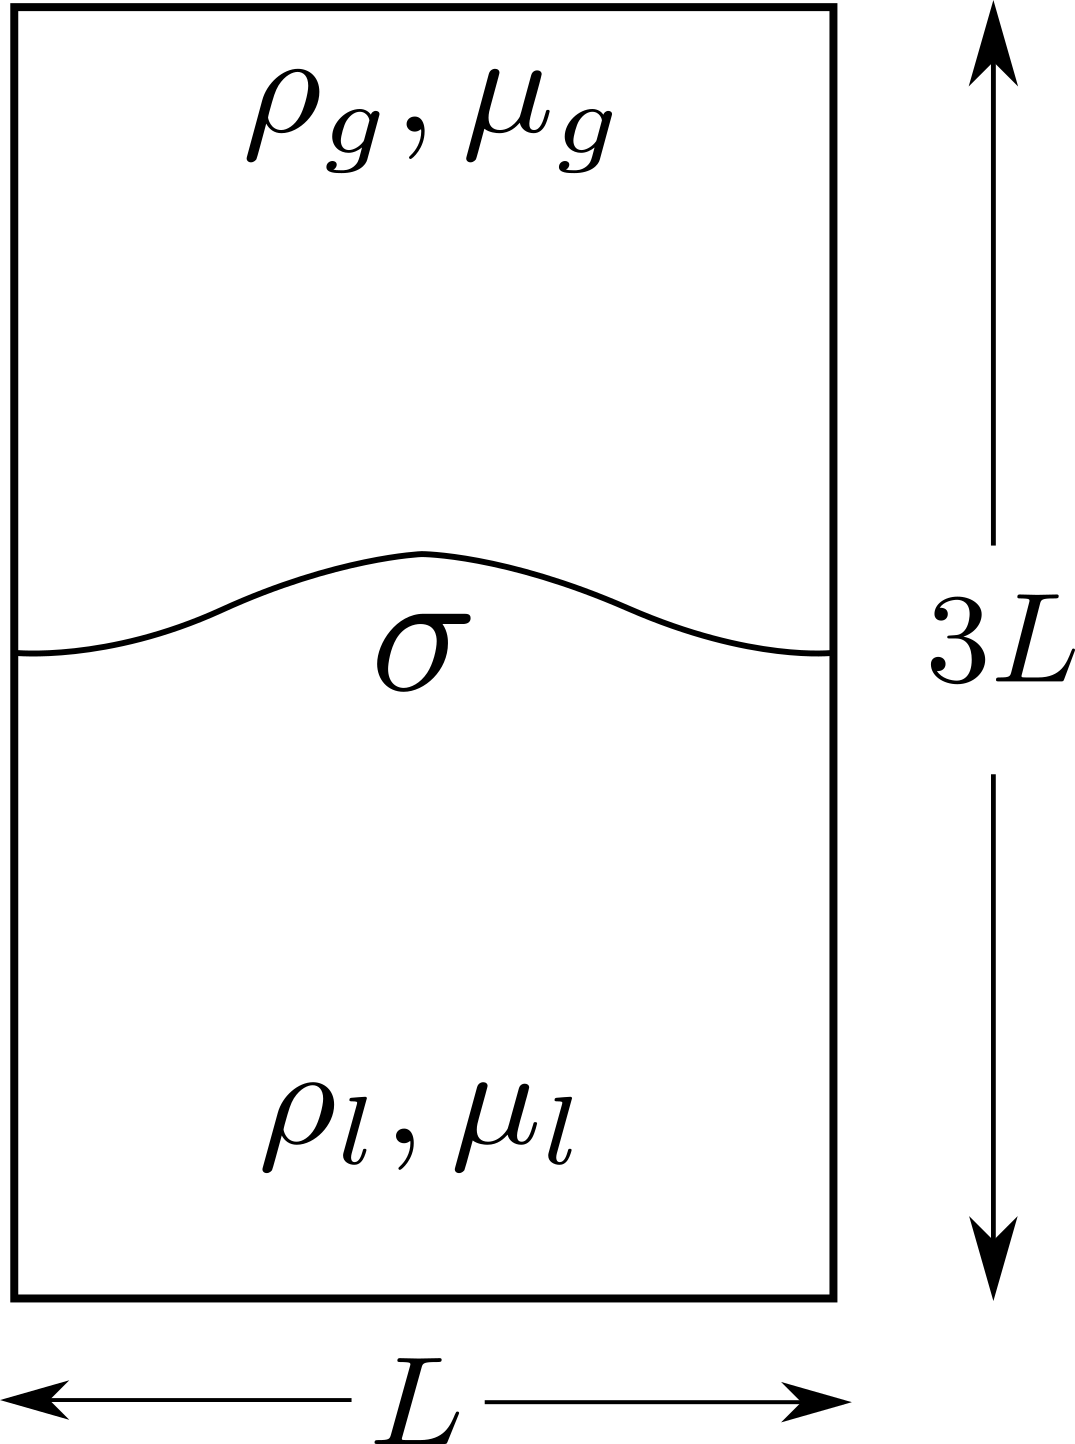
\includegraphics[width = 1.0\textwidth]{plots/capwave/capwave_conf.png}
	\caption{Schematic of the initially perturbed planar interface separating two immiscible fluids of different densities and viscosities. A spatial resolution of $32 \times 96$ is used for spatial discretization (compared to $64 \times 192$ in Popinet \cite{popinet2009accurate}), with the width of the box corresponding to the size of the perturbed wavelength.}
    \label{capwave_conf}
\end{figure}

In the present study, we evaluate the accuracy of our class of methods by comparing with an analytical solution of damped capillary oscillations. Generally, analytical solutions exist only for cases corresponding to extremely small initial perturbations, that too either in the inviscid limit (Lamb \sidecite{lamb1993hydrodynamics}) or the asymptotic limit of vanishing viscosity (Prosperetti \sidecite{prosperetti1980free,prosperetti1981motion}). For our purposes, we use the configuration of the viscosity-damped capillary oscillations of a planar interface, as was first implemented and popularized by Popinet \& Zaleski \cite{popinet1999front}.  

We consider a rectangular domain of dimensions $L \times 3L$, where $L$ corresponds to the wavelength of our initial perturbation. The densities of the heavier and lighter phases are $\rho_l$ and $\rho_g$ respectively, likewise for the viscosities $\mu_l$ and $\mu_g$, and $\sigma$ being the surface tension coefficient (fig. \ref{capwave_conf}). An intial perturbation amplitude of $L/100$ is used, coupled with a numerical resolution given by $L/\Delta x= 32$ ($\Delta x$ being the grid size). Symmetry conditions are applied on the top and bottom sides, with periodic conditions along the horizontal direction. We use the following adimensional parameters to characterize our problem : 

\begin{align}
	T_0 = T \omega_0 \quad , \quad \textrm{La} = \frac{\rho_l \sigma L}{\mu_l^2}  
\end{align}

where $\textrm{La}$ is the Laplace number based on the heavier fluid, and $\omega_0$ is defined using the dispersion relation used in Popinet \cite{popinet2009accurate} given as : 

\begin{align}
	\omega_0^2 =  \frac{\sigma k^3}{2 \rho_l} \quad, \qquad \text{where} \quad k = \frac{2\pi}{L}   
\end{align}

The dispersion relation is obtained via linear stability analysis at the inviscid limit \sidecite{lamb1993hydrodynamics}. In order to evaluate the influence of density-ratio on the performance of our class of methods, we use three different numerical setups keeping the same Laplace number ($\textrm{La} = 3000$) as follows : 

\begin{itemize}
	\item $\rho_l/\rho_g = 1$ , $\mu_l/\mu_g = 1$  (Popinet \cite{popinet2009accurate}) 
	\item $\rho_l/\rho_g = 10$ , $\mu_l/\mu_g = 1$   
	\item $\rho_l/\rho_g = 1000.0/1.2$ , $\mu_l/\mu_g = 1.003\cdot 10^{-3}/1.8\cdot 10^{-5}$ (Air-Water) 
\end{itemize}

The final setup corresponds to that of an air-water interface (physical properties corresponding to $20^o$ Celsuis), which is the most stringent due to the significant density and viscosity jumps. 

\subsection*{Comparison with Prosperetti Solution}

The theoretical solution to this configuration corresponds to the closed-form expressions of the planar interface shape evolution established by Prosperetti \cite{prosperetti1981motion,prosperetti1980free}, which takes into account the finite time-scales at which the vorticity (generated due to interface oscillations) diffuses into the bulk medium. These closed-form expressions are subsequently integrated using a fourth-order Runge-Kutta time integrator (details of which not described here), and used to assess the accuracy of the results obtained by our class of numerical methods. 


\begin{figure}[h!]
    \centering
    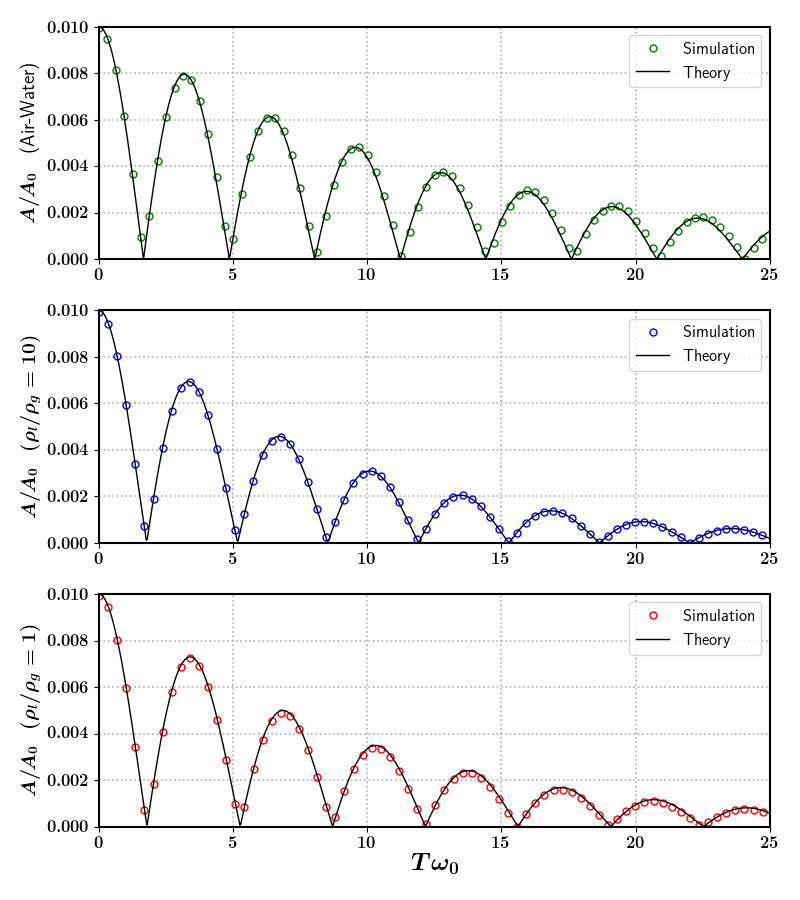
\includegraphics[width = 1.0\textwidth]{plots/capwave/compare_nonmc.png}
	\caption{\textbf{STD} Time evolution of the amplitude of the planar interface undergoing damped capillary oscillations, comparing the solution obtained by our numerical method with the closed-from Prosperetti solution. More or less good agreement with theory is observed for all the density-ratios tested. }
    \label{capwave_nonmc}
\end{figure}

As we can in figures \ref{capwave_nonmc} to \ref{capwave_sagar}, solutions from our class of numerical methods (circles) are compared to that of the theoretical (Prosperetti) solution (black curves), where the amplitude is normalized by the initial value ($A_0$) and the time rescaled by $T_0$. The first figure (\ref{capwave_nonmc}) refers to simulations carried out by the non-consistent method, the second (\ref{capwave_daniel}) corresponds to that of the consistent method, and the final one (\ref{capwave_sagar}) refers to that of the consistent and conservative method. We observe that there is hardly any appreciable qualitative difference between the results obtained via the different methods \textbf{STD}, \textbf{MSHIFT} and \textbf{MSUB}, although \textbf{MSUB} does seem to perforn marginally better when it comes to the most stringent case (air-water configuration). Surprisingly, even the non-consistent method (\textbf{STD}) does not seem to show any un-physical interfacial deformations for all the density-ratios tested, and that it is difficult to distinguish between the different methods for the lower density-ratios.  

\begin{figure}[h!]
    \centering
    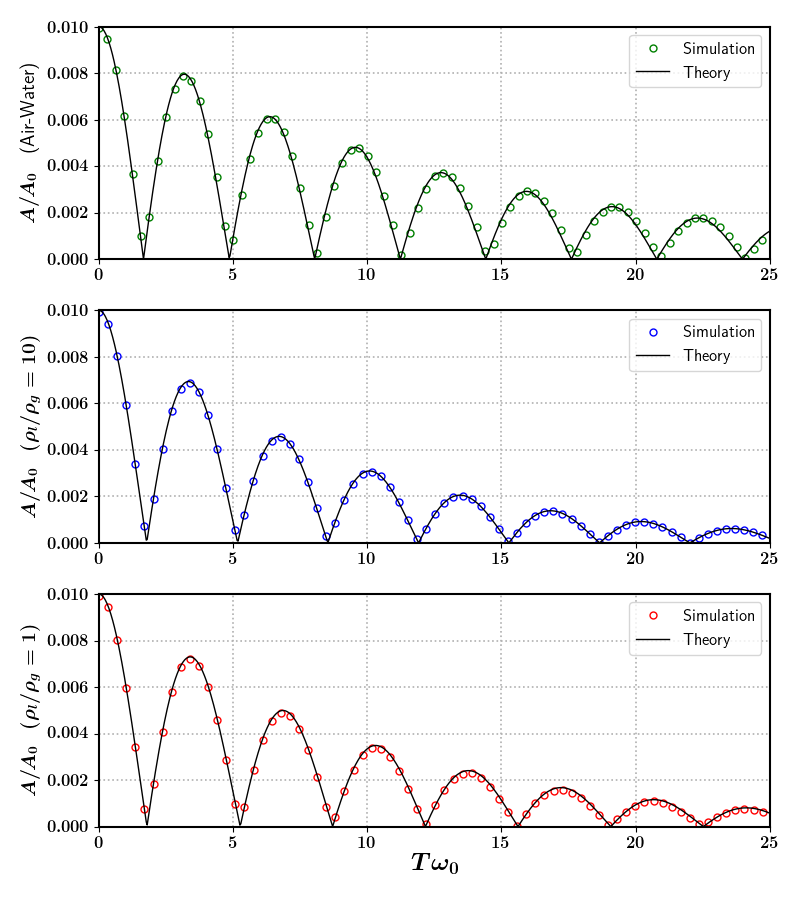
\includegraphics[width = 1.0\textwidth]{plots/capwave/compare_daniel.png}
	\caption{\textbf{MSHIFT} Time evolution of the amplitude of the planar interface undergoing damped capillary oscillations, comparing the solution obtained by our numerical method with the closed-from Prosperetti solution. Behavior is quite similar to \textbf{STD}, with good agreement with theory for all the density-ratios tested. }
    \label{capwave_daniel}
\end{figure}

\begin{figure}[h!]
    \centering
    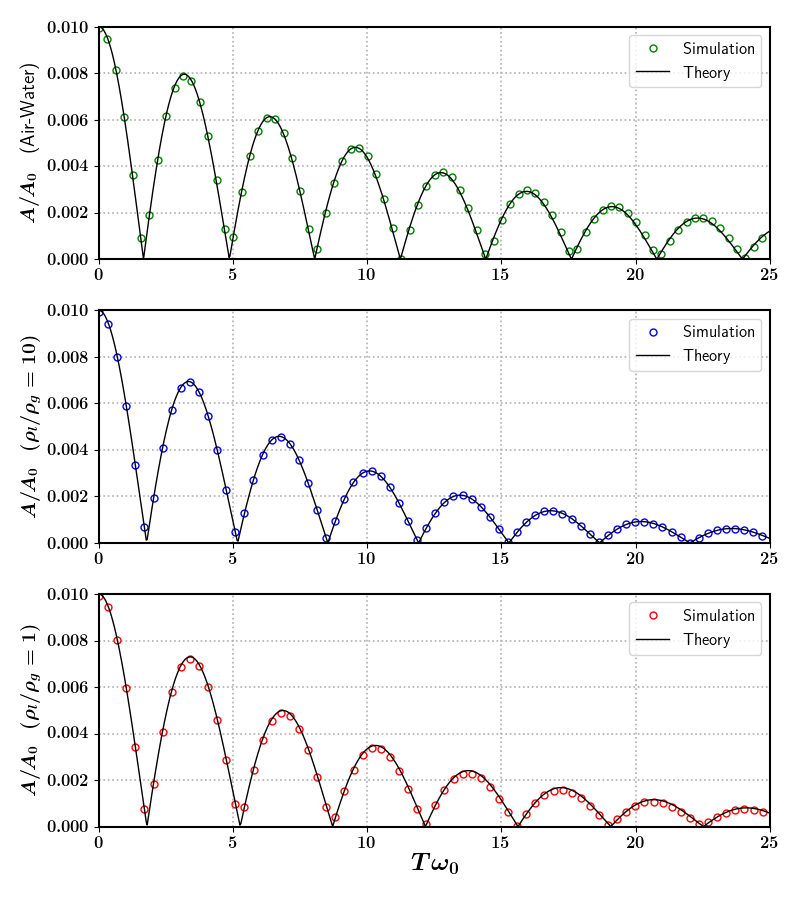
\includegraphics[width = 1.0\textwidth]{plots/capwave/compare_sagar.png}
	\caption{\textbf{MSUB} Time evolution of the amplitude of the planar interface undergoing damped capillary oscillations, comparing the solution obtained by our numerical method with the closed-from Prosperetti solution. Slightly better agreement with theory when comparing to \textbf{STD} and \textbf{MSHIFT}, for all density-ratios tested. }
    \label{capwave_sagar}
\end{figure}


\subsection*{Spatial Convergence}

The next step in our evaluation would be to quantify the accuracy of our numerical results to the Prosperetti solution using an integral (in time) error norm, the same as defined in \cite{popinet2009accurate} :       


\begin{figure}[h!]
    \centering
    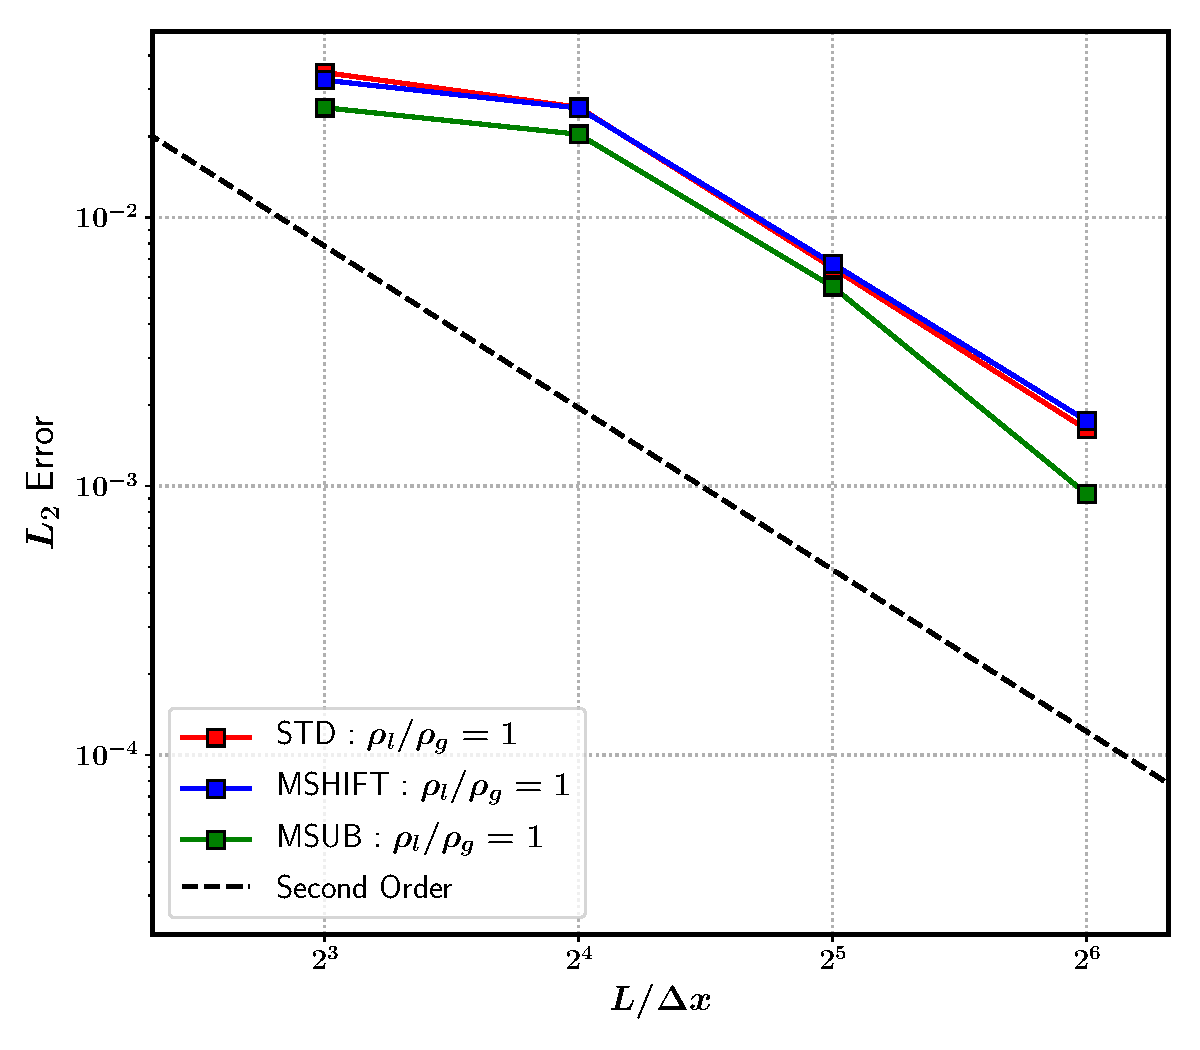
\includegraphics[width = 1.0\textwidth]{plots/capwave/conv_r1.pdf}
	\caption{Comparison of spatial convergence for the case of $\rho_l/\rho_g = 1 , \textrm{La} = 3000$, for our class of methods. There is no viscosity jump across the interface. All methods seem to demonstrate approximately second-order convergence. There seems to be no appreciable difference in the behavior of \textbf{STD} and \textbf{MSHIFT}, with \textbf{MSUB} displaying marginally lower errors compared to the others. }
    \label{conv_r1}
\end{figure}


\begin{figure}[h!]
    \centering
    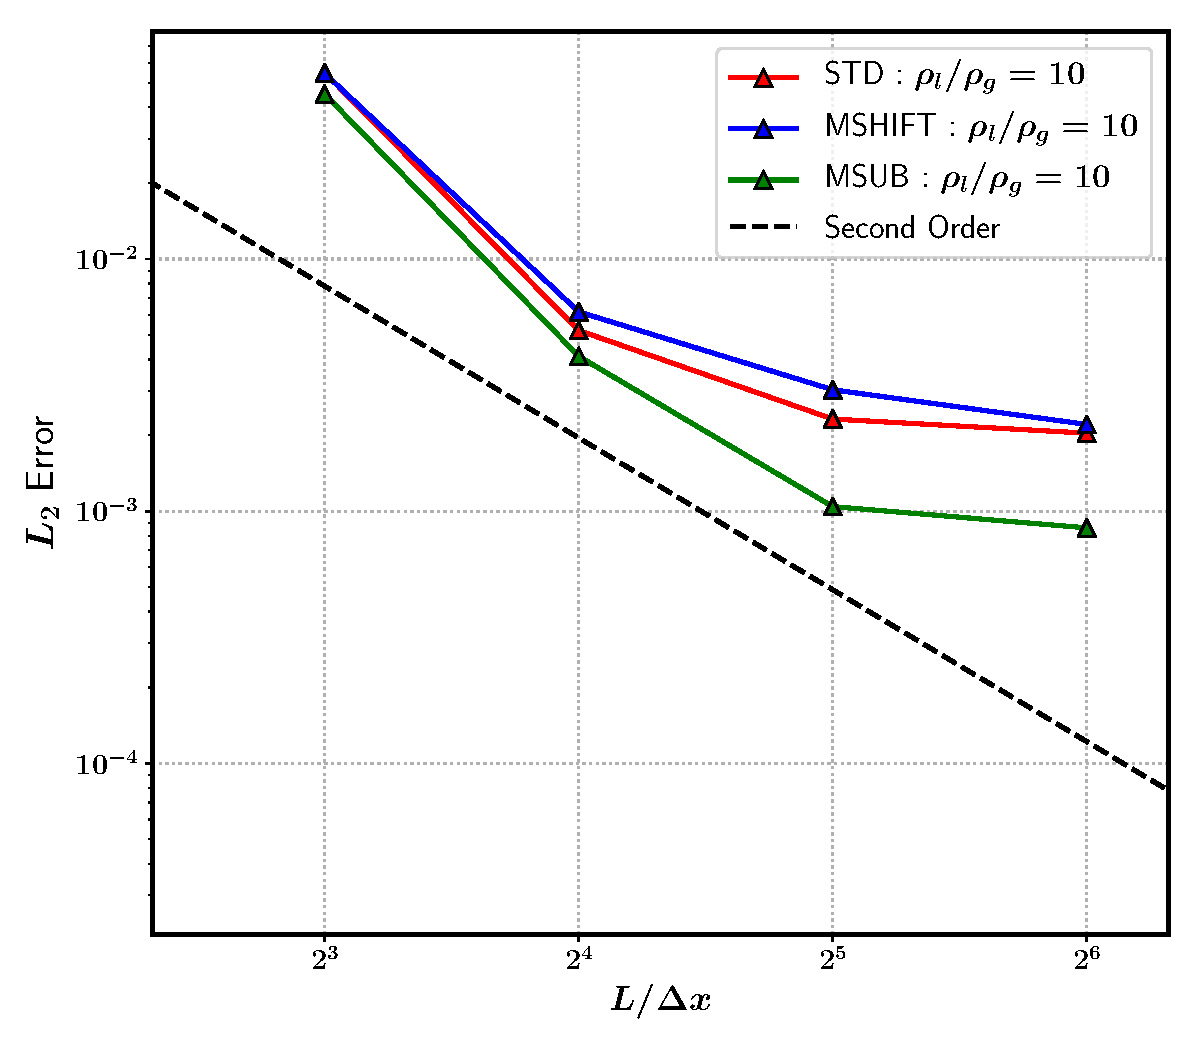
\includegraphics[width = 1.0\textwidth]{plots/capwave/conv_r10.pdf}
	\caption{Comparison of spatial convergence for the case of $\rho_l/\rho_g = 10 , \textrm{La} = 3000$, for our class of methods. Again, there is no viscosity jump across the interface. All methods seem to demonstrate approximately second-order convergence upto $ L/ \Delta x = 32 $, beyond which there is a slight saturation in the rate of convergence. Qualitatively, \textbf{STD} and \textbf{MSHIFT} demonstrate similar behavior, with \textbf{MSUB} delivering the lowest errors. In case of \textbf{MSUB}, the errors are lower by a factor of $2$ compared to \textbf{STD} and \textbf{MSHIFT} for resolutions above $L / \Delta x = 16$. }
    \label{conv_r10}
\end{figure}


\begin{figure}[h!]
    \centering
    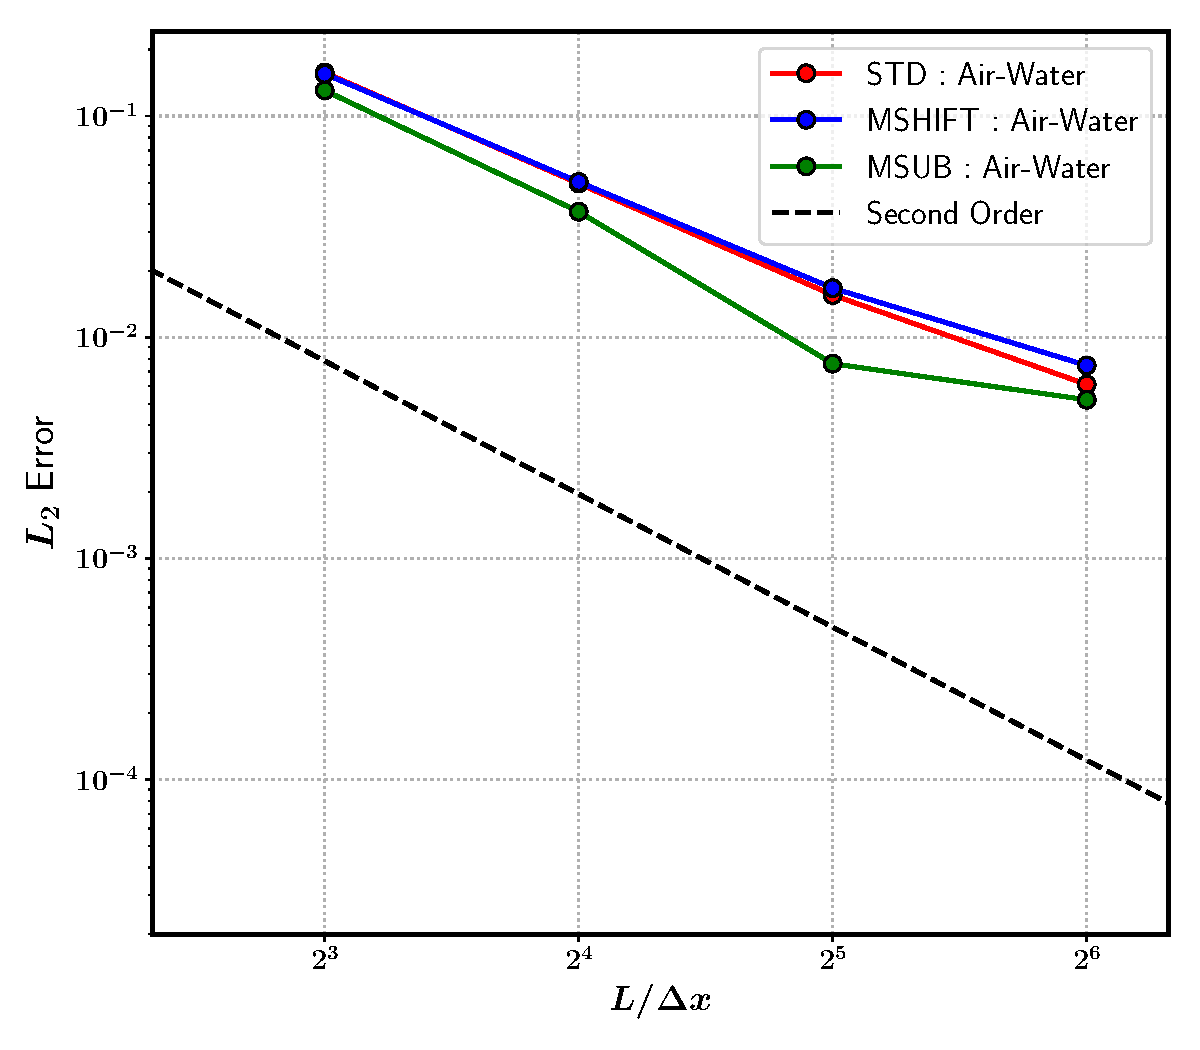
\includegraphics[width = 1.0\textwidth]{plots/capwave/conv_aw.pdf}
	\caption{Comparison of spatial convergence for the Air-Water case corresponding to $\rho_l/\rho_g = 1000.0/1.2 , \mu_l/\mu_g = 1.003\cdot 10^{-3}/1.8\cdot 10^{-5} , \textrm{La} = 3000 $, for our class of methods. All methods seem to demonstrate approximately second-order convergence. No appreciable difference is observed between \textbf{STD} and \textbf{MSHIFT}, with \textbf{MSUB} delivering slightly lower errors although there is some saturation in the convergence rate at higher resolutions. }
    \label{conv_aw}
\end{figure}

\begin{align}
	L_2 = \frac{1}{L} \sqrt{\frac{\omega_0}{25} \int_{t=0}^{T} \left(h - h_{exact}\right)^2}
\end{align}

where $h$ is the maximum inteface height obtained using our numerical simulations, and $h_{exact}$ being the maximum height obtained via time integration of the Prosperetti solution. In figures \ref{conv_r1} to \ref{conv_aw} we demonstrate the rate of spatial convergence of the $L_2$ error norms for different density-ratios, simultaneously comparing the behavior of the different methods \textbf{STD}, \textbf{MSHIFT} and \textbf{MSUB} at each density-ratio. In all the results presented, we maintain $\textrm{La} = 3000$ for all density-ratios, spatial resolutions and methods tested.  

In figure \ref{conv_r1} we observe roughly second-order spatial convergence when it comes to equal densities across the interface, with \textbf{STD} and \textbf{MSHIFT} displaying nearly identical behavior, whereas \textbf{MSUB} does marginally better with lower errors for all resolutions. When it comes to $\rho_l / \rho_g = 10$ in figure \ref{conv_r10}, we observe a saturation in the initial second-order convergence rate irrespective of whichever method is used, however \textbf{MSUB} performs much better in terms of error when compared \textbf{STD} and \textbf{MSHIFT}. Finally, figure \ref{conv_aw} demonstrates the roughly second-order convergence of all three methods when it comes to the air-water configuration, again, with \textbf{MSUB} performing marginally better with lower errors. Not surprisingly, the largest errors arise for the air-water configuration errors across all methods. 



\setchapterpreamble[u]{\margintoc}
\chapter{The Falling Raindrop}
\labch{raindrop}

The focus of the present chapter shall be to take a closer look at the issues 
plaguing numerical methods that try to deal with flows 
entailing significant density contrasts between the fluids. 
Arguably, the most common instances of such flows are those involving the interaction
between air and water, primarily in the form of droplets and 
bubbles that play important roles in both natural and industrial processes. 
As for the numerical platform, we use `PARIS Simulator' 
\sidenote{Refer to \cite{paris} for a detailed exposition  
of the numerical methods implemented in `PARIS Simulator.} 
to carry out our simulations on this topic. 
A flow configuration that combines the complexities of large 
density-ratios with the interaction between capillary, viscous and 
inertial stresses is that of a water droplet falling in 
air under the influence of gravitational acceleration.

%---------------------------------------------------------------
\section{Problem Setup}

The problem is characterized by a combination of Reynolds, 
Weber and Bond numbers, the definitions of which are as follows : 

\begin{align}
	\textrm{We}=\frac{\rho_{g} U^2 D}{\sigma} \quad,\quad \textrm{Re}= \frac{\rho_{l} U D}{\mu_{g}} \quad,\quad \textrm{Bo}=\frac{\left(\rho_{l}-\rho_{g}\right) g D^2 }{\sigma}
\end{align}

\marginnote{As the density and viscosity ratios are corresponding to that of air-water systems at 20 degree Celcius,
an equivalent characterization could be done using the Morton number $\left( \textrm{Mo} = \frac{g\mu_g^4(\rho_l-\rho_g)}{\rho_g^2 \sigma^3} \right)$ 
in place of the Bond number.}


The subscripts $l$ and $g$ represent liquid and gas phases respectively. 
In our particular numerical setup, $\textrm{We}\simeq 3.2 $, 
$\textrm{Re} \simeq 1455 $ and $\textrm{Bo} \simeq 1.2 $,
thus corresponding to that of a $3mm$ diameter raindrop (a relatively large one) 
falling in the air at an approximate terminal velocity of  
$8$ m/s (interpolated from empirical data, refer to Gunn and Kinzer \cite{gunn1949}). 
This choice of length scale of the drop is motivated by the paradigmatic value
of a near-spherical raindrop simulation, and by the fact that the corresponding Weber
number ($\sim 3$) is the same as in a similar air-water setup corresponding to  
suddenly-accelerated-droplet (or ``secondary atomization" ) simulations in the studies \cite{xiao2012,xiao2014large}.
For such a low Weber number the capillary forces dominate and the 
droplet should remain intact, and definitely not undergo any subsequent atomization. 
The parameters in the problem setup are given in Table \ref{raindropprop}, 
and the schematic diagram given in Fig. \ref{setup}. 
The droplet is initially placed at the center of a cubic domain (3D), 
where the length of the side is 4 times the diameter of the drop. 

\begin{table*}[h!]
\begin{center}
\begin{tabular}{ccccccc}
\hline\hline
$\rho_{g}$ & $\rho_{l}$ & $\mu_{g}$ 
& $\mu_{l}$ & $\sigma$ & $D$ & $g$\\
$\left(kg/m^3\right)$ & $\left(kg/m^3\right)$ & $\left(Pa \, s\right)$ 
& $\left(Pa \,s \right)$ & $\left(N/m\right)$ & $(m)$ & $(m /s^{2})$ \\
\hline
1.2 & $0.9982 \times 10^3$ & $1.98 \times 10^{-5}$ & 
$8.9 \times 10^{-4}$ & $0.0728$ & $3 \times 10^{-3}$ & $9.81$\\
\hline\hline
\end{tabular}
\caption{Parameter values used in the simulation 
	of a falling water droplet in air. \label{raindropprop}}
\end{center}
\end{table*}


In order to properly reproduce and analyse the dynamics 
of a relatively large drop (high Reynolds flow) such as in our case, 
the numerical method has to accurately resolve the thin boundary layers 
\sidenote{Even for simulations with 60 points across the droplet diameter, 
the boundary layer has only by 3-4 cells across it. }, 
the interaction of such layers with the capillary forces and finally 
the non-linear feedback of the complex 
3D vortical structures present in the wake behind the droplet.
Arguably, the most natural type of computational setup would involve using 
a large domain filled with air at rest, with zero inflow velocity and to
let the droplet fall from the top of the domain.
Such an undertaking was attempted by Dodd and Ferrante \cite{dodd2014}, 
in which they managed to delineate the different regimes concerning the 
behavior of the wake behind the droplet, although at relatively 
lower Reynolds numbers corresponding to smaller drops 
(the maximum Reynolds tested was $\simeq 500$, whereas in our case it is $\simeq 1500$).    
We on the other hand use a significantly smaller domain ($L/D = 4$ where $L$ is the domain size), 
with a constant value of inflow velocity (close to $8$ m/s), thus resulting in the drop 
exiting the domain after a certain amount of time. 
This setup proves to be quite convenient for relatively short-time investigations.
Therefore, our objective behind the demonstration of this particular 
test case is \textit{not} to develop a high fidelity model of a raindrop 
\sidenote{In the Dodd and Ferrante \cite{dodd2014} study , 
a droplet was allowed to fall from rest
along a domain with a length corresponding to 32 times the droplet diameter, 
therefore necessitating a problem size of approximately 260 million cells.}, 
but rather carry out a stringent evaluation of the robustness of our class of 
numerical methods (shifted fractions and sub-grid strategies) 
compared to the standard version of the method that is not mass-momentum consistent. 

% -----
\begin{figure}[h!]
\begin{center}
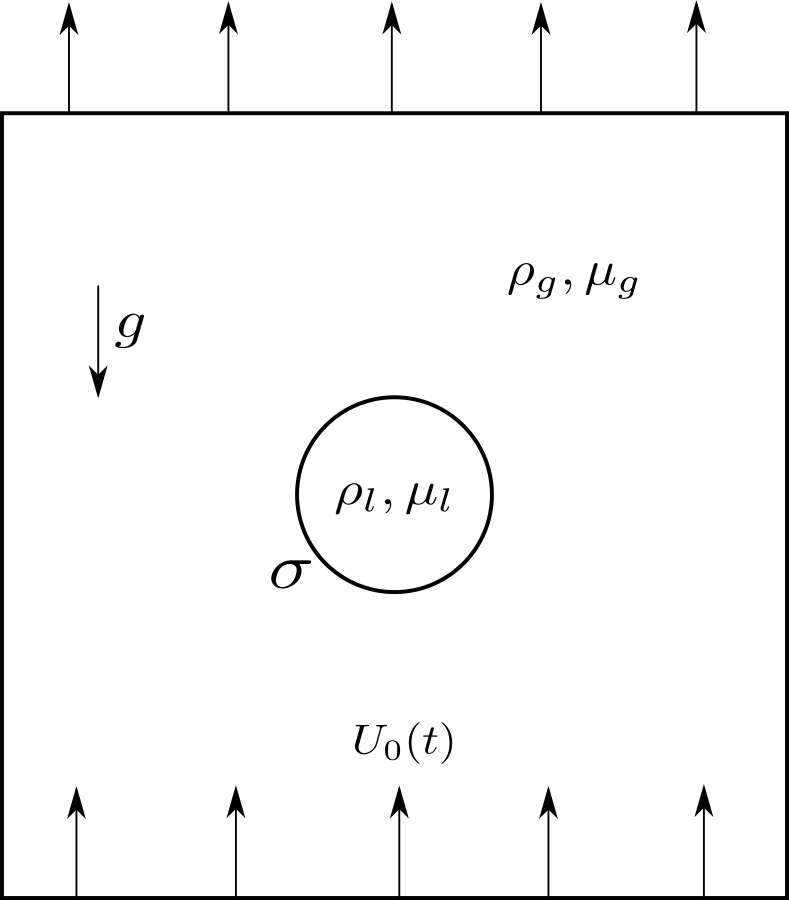
\includegraphics[width=0.5\textwidth]{plots/raindrop/setup.png}
\end{center}
\caption{A 2D schematic of the numerical setup for the falling raindrop. 
	A droplet of diameter $D$ is placed at the center of a cubic domain 
	of side $L$ and $L/D = 4$. The liquid properties ($\rho_l$ , $\mu_l$) 
	correspond to that of water, and the gas properties ($\rho_g$,$\mu_g$) 
	correspond to that of air. We apply a uniform inflow velocity condition 
	with $U_0(t)$ and an outflow velocity condition at the top which 
	corresponds to zero normal gradient.
	Boundary conditions on the side walls correspond 
	to those of impenetrable free slip (no shear stress).}
\label{setup}
\end{figure}

%---------------------------------------------------------------
\section{Numerical Instabilities}

Numerical simulations using a fixed inflow velocity with $U_0(t) = 8 $ m/s 
were carried out for very short times (of the order of 1ms) at moderate resolution 
\sidenote{Droplet resolutions between $D/h = 16$ to $D/h = 64$ are considered
to be moderate, where $D$ is the droplet diameter and $h$ is the grid size.}.
The simulations carried out with the standard version of our numerical method 
result in the catastrophic deformations of the droplet as illustrated in Fig. \ref{explode_compare}, 
which we describe as ``fictitious" or ``artificial" atomization. 
They display marked peaks or spikes in kinetic energy as a function of time, 
associated with massively deformed interface shapes (see figure \ref{explode_compare}). 
Additionally, our studies suggest that certain combinations 
of the advection scheme and the flux limiter are 
numerically more robust than others
,in particular, the most stable combinations 
are that of CIAM advection with 
Superbee limiter, and the WY advection with QUICK limiter. 

\subsection*{Instability Mechanism}

We propose the following explanation in order to account for such numerical artifacts. 
To start with, we neglect gravity and viscous effects at this relatively large Reynolds number. 
Also, we are interested in steady-state flow 
\sidenote{As the simulation starts with uniform flow in the gas and a zero velocity
in the drop, there is a sudden large acceleration in the gas, resulting in the development 
of a dipolar velocity field akin to that of potential flow around a cylinder (sphere). }. 
On the axis and near the hyperbolic stagnation point 
at the front of the droplet one has $u_2=0$ for the transverse 
(radial) velocity and for the axial momentum balance


\begin{align}
u_1 \partial_1 u_1 = - \frac 1 \rho \partial_1 p.
\end{align}

Due to the large viscosity and density ratios, it is not possible for 
the air flow to immediately entrain the water, so the fluid velocity 
is significantly smaller inside the droplet. 
In the air the acceleration near the stagnation point is 
of the order $U^2/D$, whereas the pressure gradient is

\begin{align}
\partial_1 p \sim \rho_{g} U^2/D.
\end{align}

The pressure gradient in the liquid is much smaller, 
however, in the case of a mixed cell the water density 
may multiply (due to numerical errors) with the gas acceleration $U^2/D$, so that

\begin{align}
\partial_1 p \sim \rho_{l} U^2/D,
\end{align}

then a large pressure gradient results in the mixed cell or cells. 
This large pressure gradient results in pressure spikes inside the 
droplet near the front stagnation point, as shown in Figure \ref{pressure_1}. 
Such pressure gradients are balanced by surface tension only for a sufficiently 
large curvatures near the droplet front. 
This explains the presence of a ``dimple'' often observed in low 
resolution simulations of the falling drop. 
This artifact had been observed by Xiao \cite{xiao2012} in a similar case
\sidenote{In the thesis of Xiao, the focus was on the analysis of droplet breakup 
corresponding to different Weber number regimes.}
involving the sudden interaction of a droplet at rest with a uniform gas flow. 
The resulting large un-physical pressure gradients across the interface 
eventually lead to its rapid destabilization and concomitant breakup.  

\begin{figure*}
\begin{center}
\begin{tabular}{cc}
\hspace*{-1.0cm}
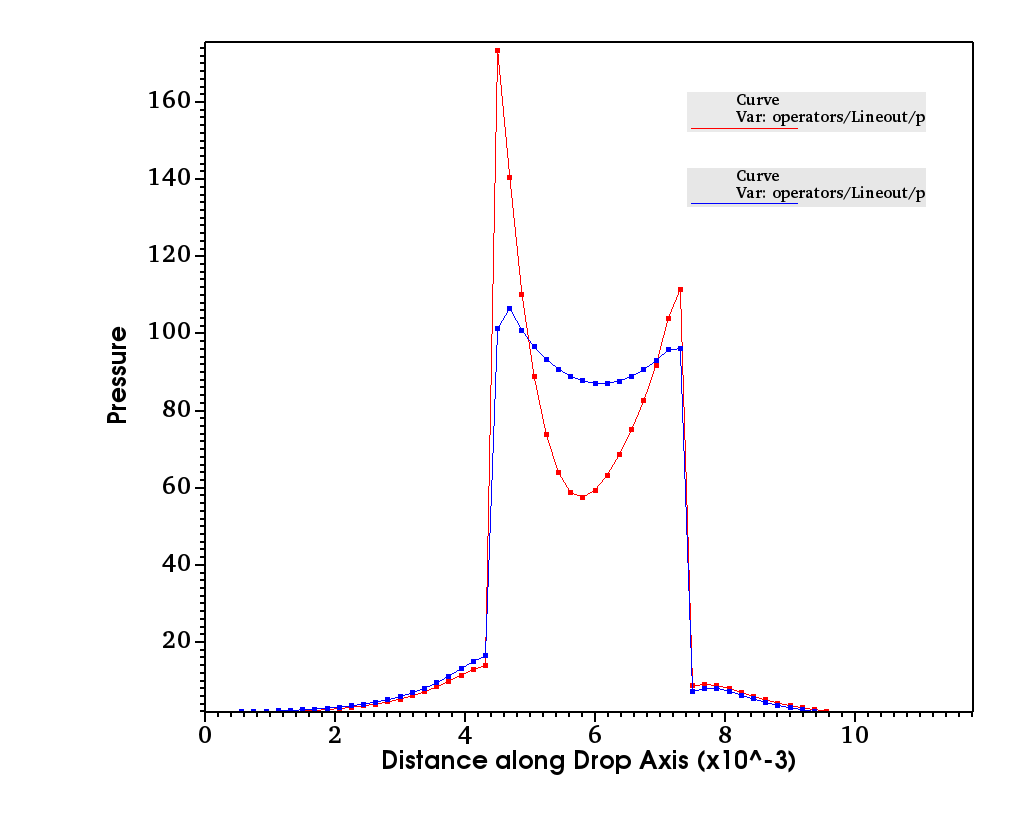
\includegraphics[width=0.8\textwidth]{plots/raindrop/pressure_compare.png} &
\hspace{-0.4cm}%
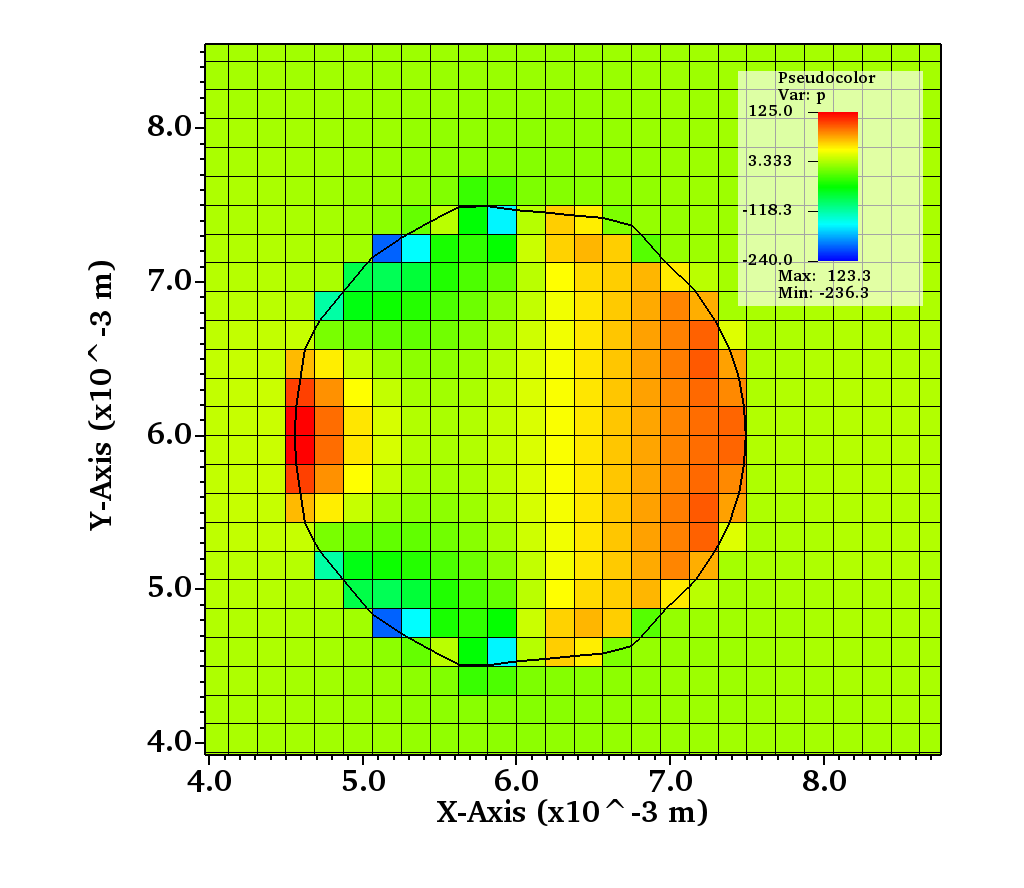
\includegraphics[width=0.8\textwidth]{plots/raindrop/nonmc_16ppd_pressure.png}\\
\hspace{-0.8cm}%
(a) & (b)
\end{tabular}
\end{center}
\caption{The origin of the pressure peak in the front of the droplet. 
(a) The profile of the pressure on the axis a few timesteps after initialisation 
with the standard, non-consistent method (red curve) and the consistent method based
on the shifted fractions (\textbf{MSHIFT}) strategy (green curve). 
Much larger pressure gradients are present across the interface using the non-consistent method. 
(b) The pressure distribution immediately after the start of the simulation 
using the standard, non-consistent method. The pressure peak has not yet resulted
in the formation of a dimple. In all figures the droplet resolution corresponds to $D/h = 16$.
The simulations are carried out with the CIAM advection method, in conjunction with the Superbee limiter.}
\label{pressure_1}
\end{figure*}

\begin{figure*}
\begin{center}
\begin{tabular}{cc}
\hspace*{-1.0cm}
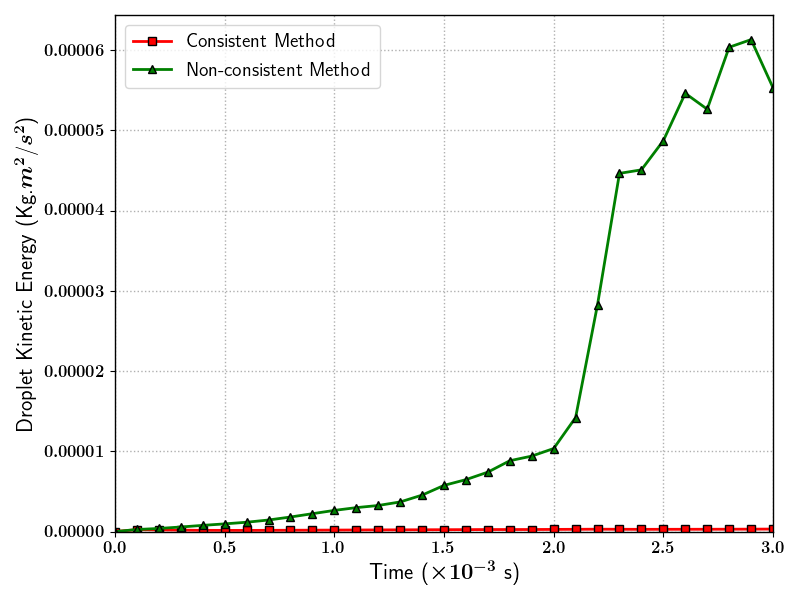
\includegraphics[width=0.8\textwidth]{plots/raindrop/ke_compare.png} &
\hspace{-0.4cm}%
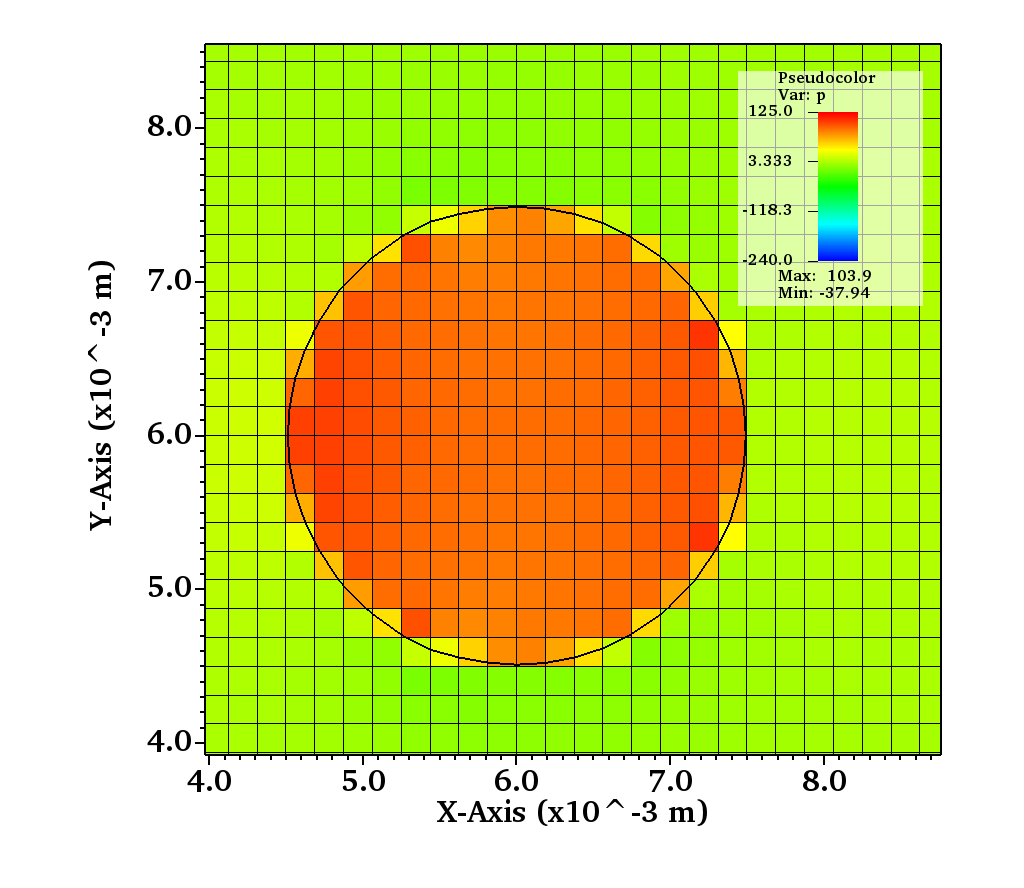
\includegraphics[width=0.8\textwidth]{plots/raindrop/mc_16ppd_pressure.png}\\
\hspace{-0.8cm}%
(a) & (b)
\end{tabular}
\end{center}
\caption{ (a) Comparison of the temporal evolution of droplet kinetic energy. 
The standard non-consistent method displays spikes in the kinetic energy that are 
approximately 3 orders of magnitude larger than that of the consistent method, 
leading to rapid destabilization. 
(b) The pressure distribution immediately after the start of the simulation 
using the consistent method based on the shifted fractions (\textbf{MSHIFT}) strategy. 
In all figures the droplet resolution corresponds to $D/h = 16$.
The simulations are carried out with the CIAM advection method, in conjunction with the Superbee limiter.}
\label{pressure_2}
\end{figure*}

\begin{figure*}
\begin{center}
\begin{tabular}{cc}
\hspace*{-1.0cm}
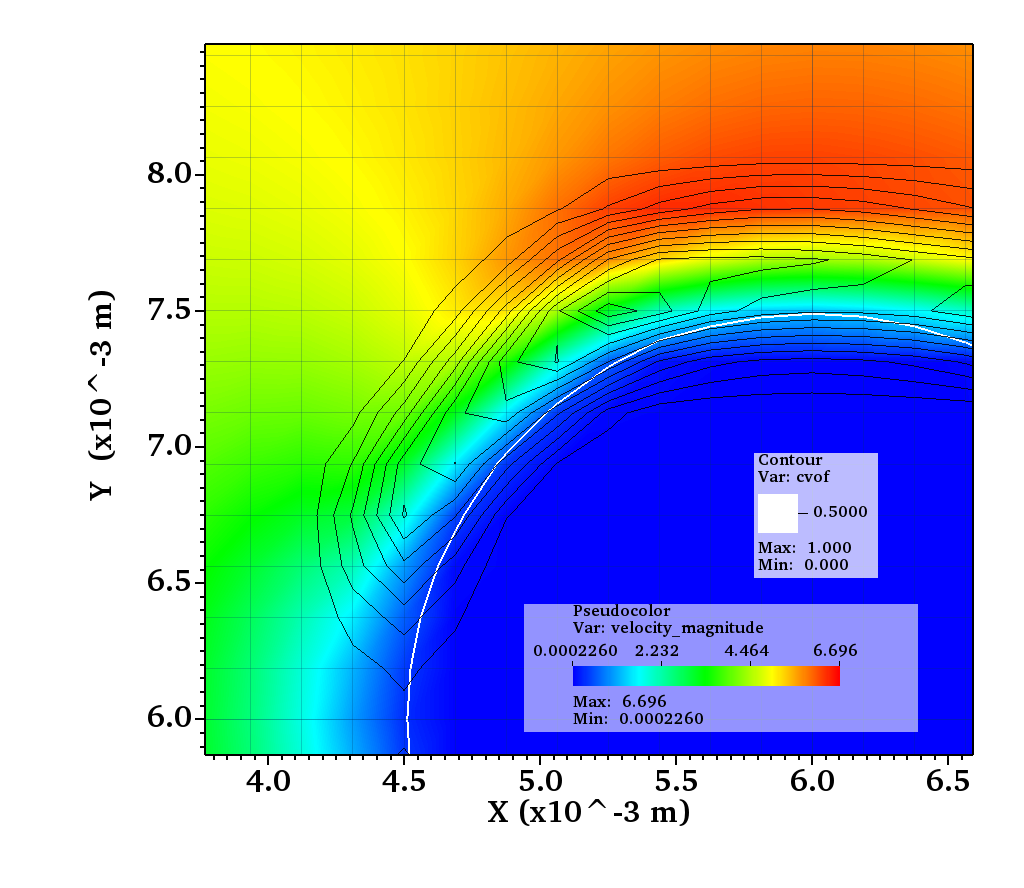
\includegraphics[width=0.8\textwidth]{plots/raindrop/mc_vorticity_zoom.png} & 
\hspace{-0.4cm}%
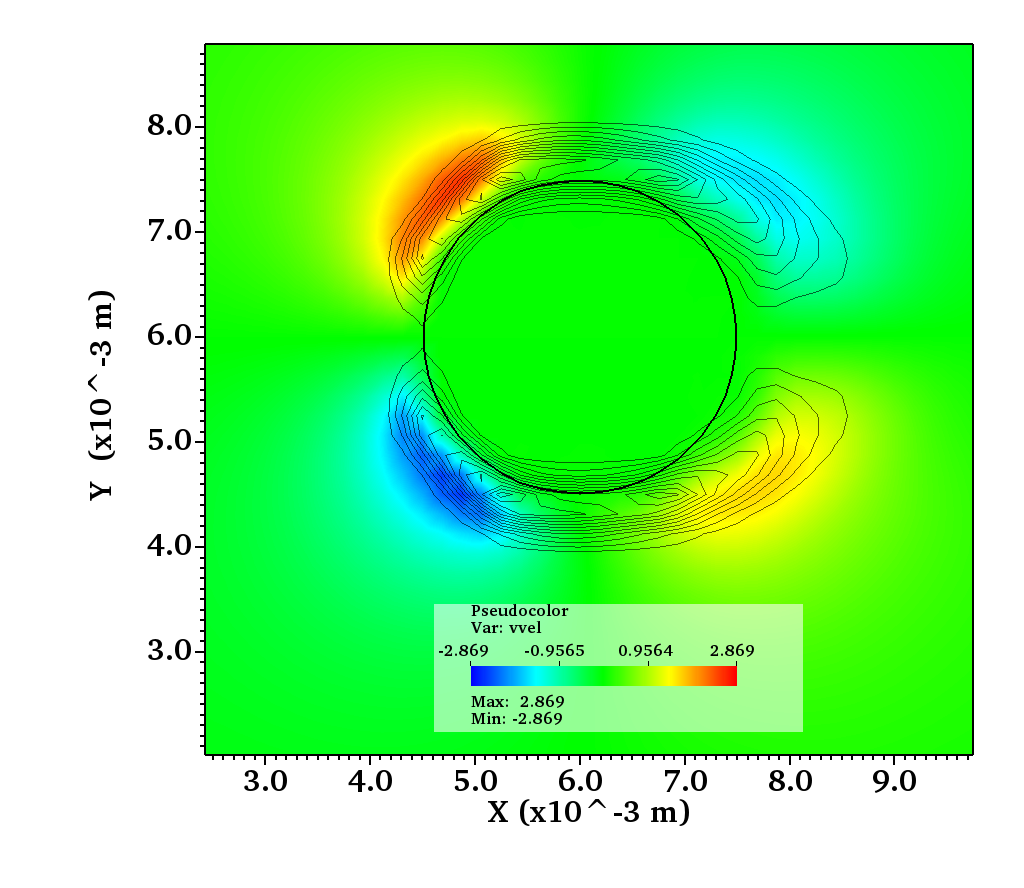
\includegraphics[width=0.8\textwidth]{plots/raindrop/mc_vorticity.png} \\ 
\hspace{-0.8cm}%
(a) & (b)
\end{tabular}
\end{center}
\caption{Flow field around the $3 mm$ droplet with $D/h = 16$ immediately 
after the start of the simulation with the consistent method (\textbf{MSHIFT}), 
demonstrating the contours of the norm of the vorticity field (black lines) . 
The 2D cross-section in these figures corresponds to the 
mid-plane slice along the Z axis, where the inflow is along 
the X axis and gravity opposite to it. (a) The velocity magnitude. 
As one can observe, the boundary layer is resolved by only 2-3 cells. 
(b) The velocity component in the Y direction, perpendicular to the flow. 
As the flow develops further, a marked separation of the boundary layers is observed with 
a more complex vortical region in the wake.
The figures correspond to simulations carried out with the 
CIAM advection method, in conjunction with the Superbee limiter.}
\label{flow_field}
\end{figure*}


Visualization of the flow around the droplets (Figure \ref{flow_field}) 
illustrates the challenging nature of the flow configuration, 
even for such a seemingly simple physical problem. 
As one can observe, the thin boundary layers are poorly resolved. 
Therefore, even though the velocity field is continuous across the 
interface (in the discrete sense) in the absence of mass transfer, 
there is the appearance of strong velocity variations at the 
scale of the grid size for such coarse levels of grid refinement. 

\begin{figure*}
\begin{center}
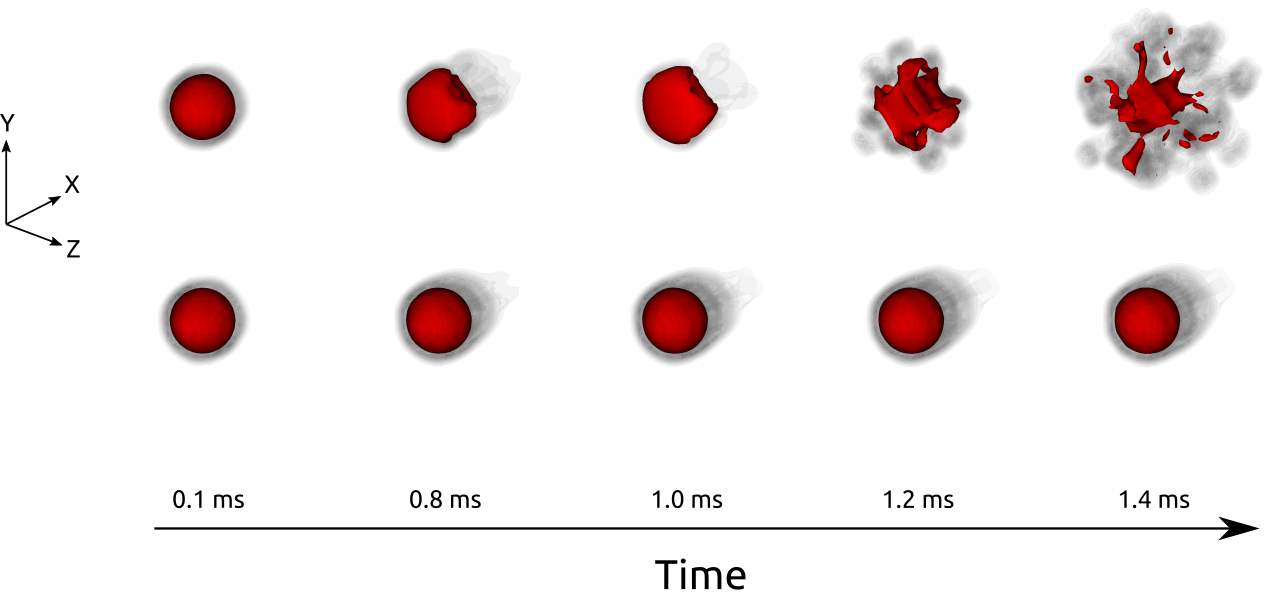
\includegraphics[width=1.25\textwidth]{plots/raindrop/raindrop_explode.png}
\end{center}
\caption{A comparison of the temporal evolution between the standard 
non-consistent method (top row) and the consistent method based on the 
shifted fractions (\textbf{MSHIFT}) strategy (bottom row), 
using the combination of CIAM advection scheme coupled with the Superbee flux limiter. 
The flow is along the positive X direction, with gravity along the opposite direction. 
The red contour indicates the isosurface of the volume fraction 
field corresponding to a value of $0.5$, whereas the black contours 
surrounding the drop represent isosurfaces of the magnitude of vorticity. 
The raindrop with the non-consistent method displays massive deformations 
leading to artificial breakup as a result of rapidly growing numerical instabilities. 
The droplet resolution for both methods is $D/h = 16$ .
The temporal evolution in case of the sub-grid based consistent method (\textbf{MSUB}) produces 
almost indistinguishable figures (bottom row), hence are not shown here.}
\label{explode_compare}
\end{figure*}


%---------------------------------------------------------------

\section{Stabilization Strategies}

The cascading nature of the numerical instabilities that lead to 
the eventual (un-physical) fragmentation of a droplet is not just a 
cause of concern in the context of modeling a raindrop, but it has important
implications within the more broader scope of 
atomization and other complex fragmentation phenomena. 
Arguably, the most important objective of numerical investigations of physical
phenomena involving fragmentation is the quantification of the size of 
the features that result from a series of topological changes 
A typical example is the statistical distributions of drop sizes. 
As demonstrated in the present study, using the standard non-consistent method  
one observes artificially atomized drops thus leading to the generation of a large number of 
smaller fragments, which if counted, will skew the resulting droplet size 
distributions towards the smaller sizes.
Therefore, we assert that the falling raindrop case serves as a faithful representation of the 
numerous under-resolved features that are typically omnipresent in
numerical studies of complex fragmentation phenomena.  
The inability to discern between the drops resulting from physically consistent 
mechanisms and those that result from numerical fragmentation is exactly
why there is a need to develop numerical schemes that circumvent the occurrence
of such instabilities, especially as there will always be some constraints in computational power.  


\subsection*{Consistent Mass-Momentum Transport}

The most common and brute force approach that one can apply 
in order to suppress or circumvent such numerical instabilities is 
by using a combination of extremely refined meshes coupled with large domains \cite{dodd2014}.
A more computationally efficient approach might be to use a 
conservative formulation
\sidenote{A prerequisite of methods that use consistent mass-momentum transport 
is the formulation of the convective operators in the conservative manner i.e
divergence of fluxes instead of gradients of the primary (discontinuous) variables.} 
of the Navier-Stokes equations, in order
to achieve consistency in the discrete transport of mass and momentum. 
A thorough and detailed exposition of the principles
behind the consistent methods and the different strategies towards achieving consistent
transport has already been covered in the preceding chapter.  
We observe that the use of our class of consistent methods 
enables us to stabilize a majority of the numerical
instabilities and bring a systematic improvement over wide range of 
flux limiters (WENO, ENO, Superbee, QUICK, Verstappen) 
and CFL numbers, as evidenced by comparing the figures \ref{pressure_1} and \ref{pressure_2}. 

\begin{figure}
\begin{center}
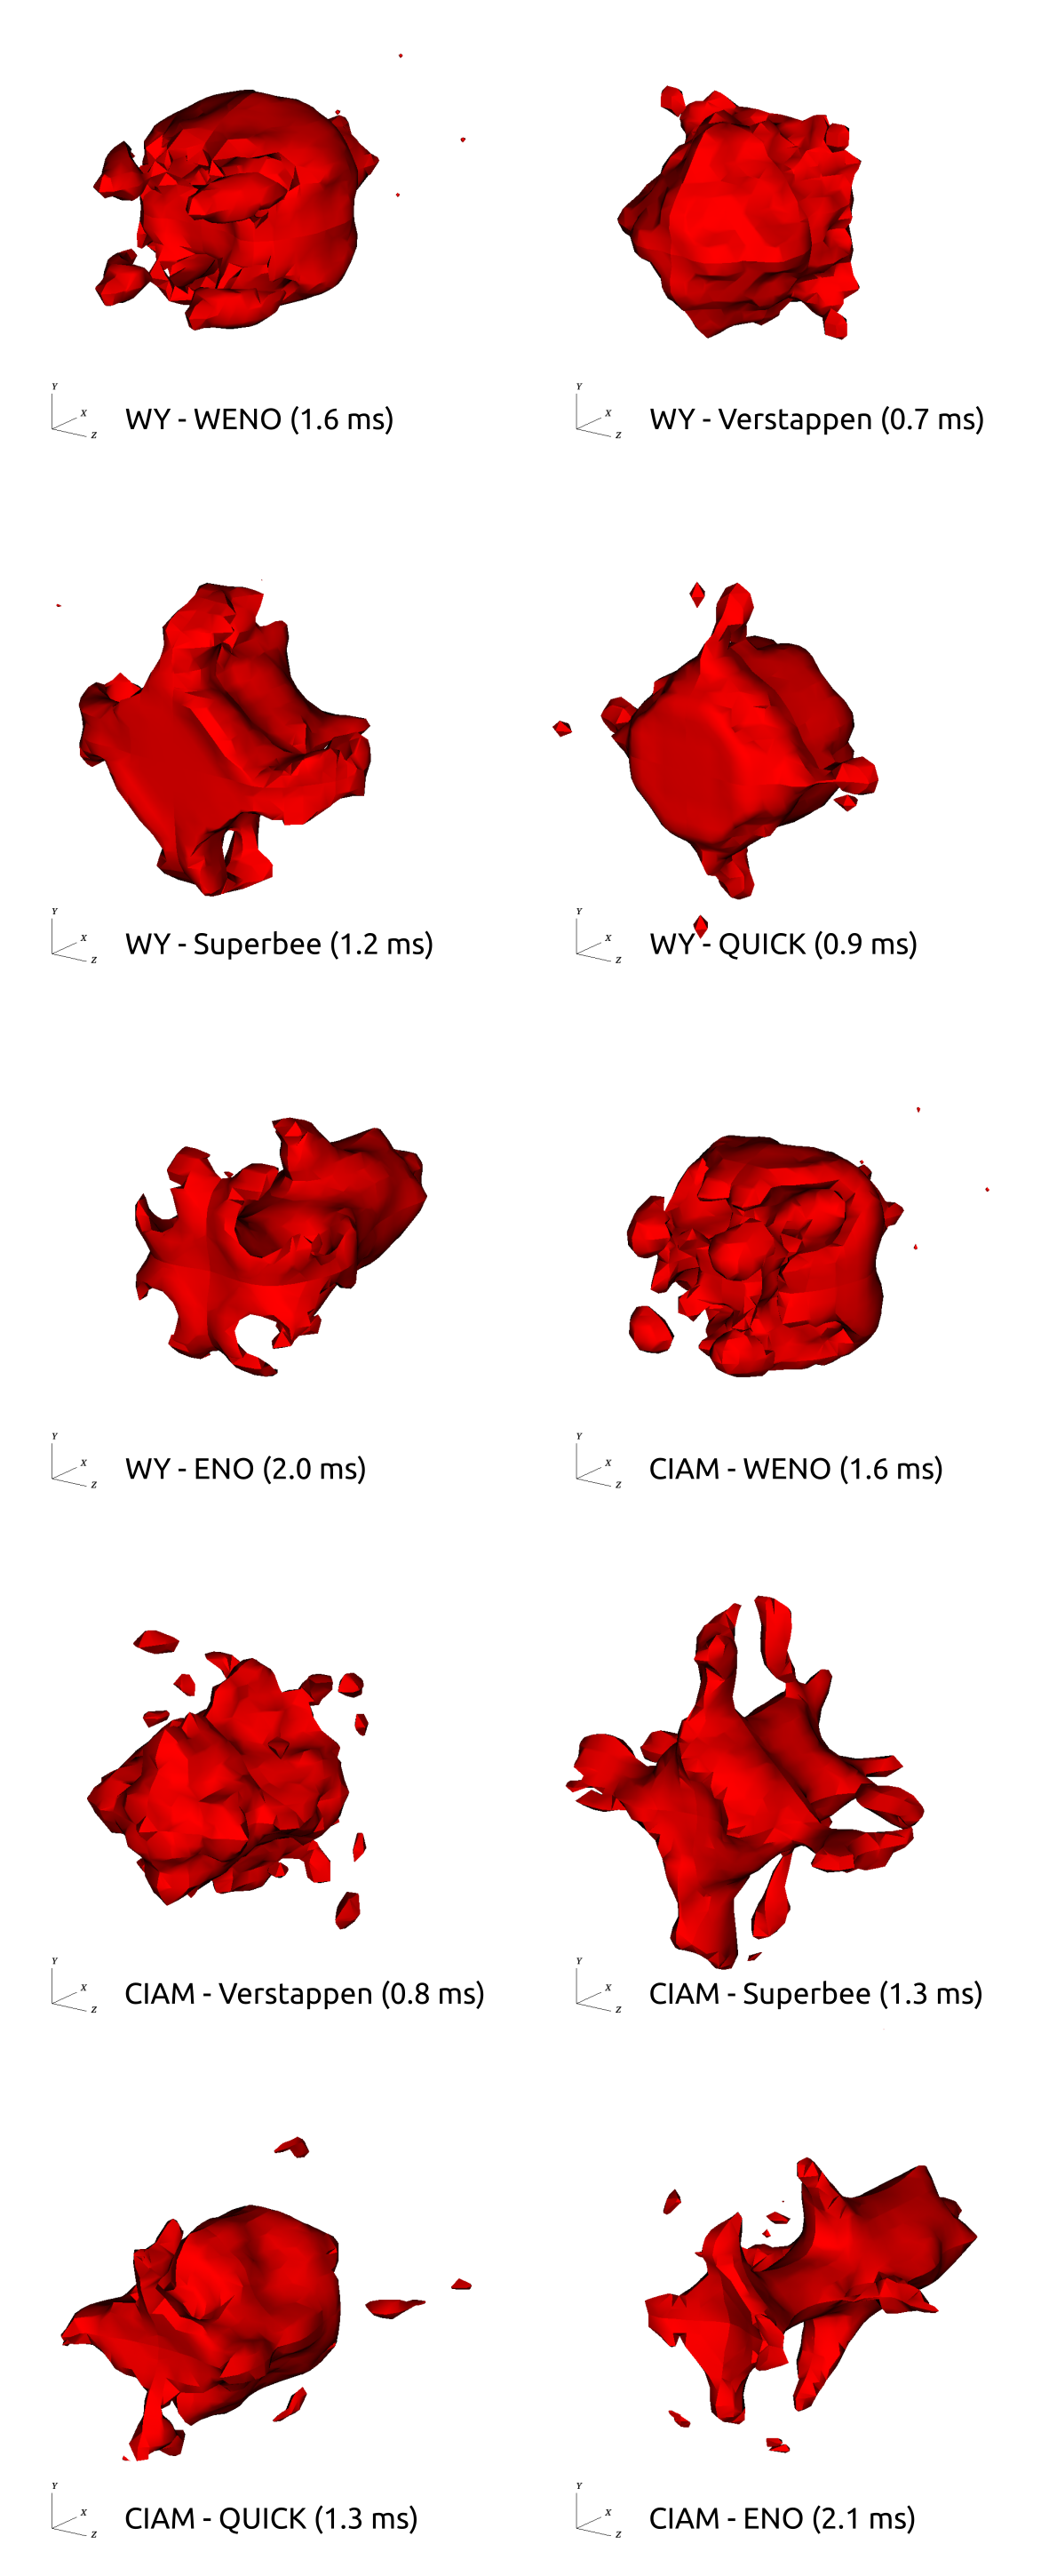
\includegraphics[width = 1.0\textwidth]{plots/raindrop/combined_failures_raindrop.png}
\end{center}
\vspace*{-0.5cm}
\caption{A juxtaposition of the different manifestations of  
`artificial' atomization one encounters while using the standard 
method (\textbf{STD}) that does not involve consistency between the discrete transport of mass and momentum. 
The red contours indicate the isosurface of the volume fraction 
field corresponding to a value of $0.5$, acting as a good proxy for the exact interfacial position. 
One can clearly observe that the un-physical fragmentation of the raindrop is symptomatic 
of the non-consistent method, systematically across all combinations of flux limiters and advection schemes. 
The symbol ``WY'' in the legend corresponds to those run using 
the Weymouth-Yue advection scheme, and ``CIAM'' corresponds to the CIAM scheme. 
Brief descriptions of these advection schemes can be found in the preceding chapter \ref{ch:method}.
The implementation of the non-linear flux limiters i.e WENO, ENO, QUICK, Superbee, Verstappen 
correspond to that of well established methods developed to 
deal with hyperbolic conservation laws, for more details refer to the
studies of Leveque \cite{flim_1} and Sweby \cite{flim_2}.
The time stamps are indicative of the moments at which the interface
is the most deformed, and do not necessarily correspond to the moment
at which the code crashes.} 
\label{explode_all}
\end{figure}

% multiplot caf_paper
\begin{figure*}
\begin{center}
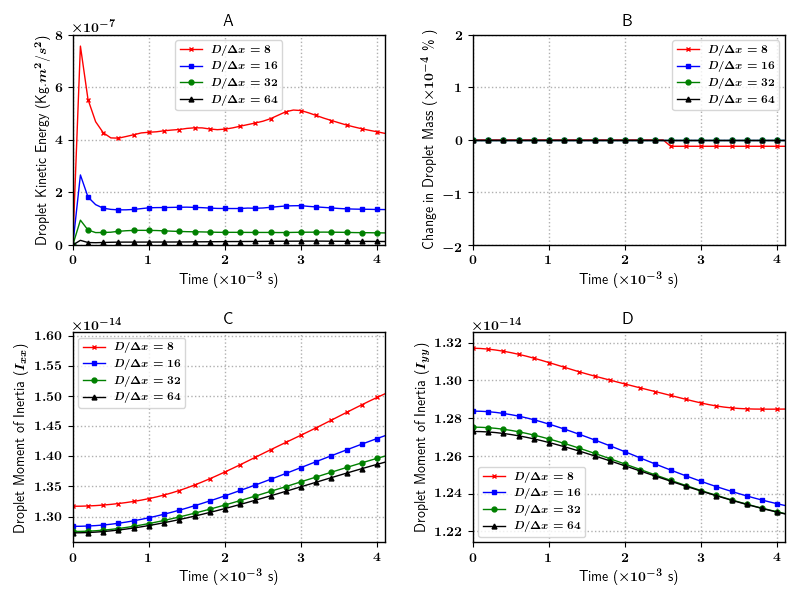
\includegraphics[width = 1.5\textwidth]{plots/raindrop/multiplot_raindrop.png}
\end{center}
\vspace*{-0.5cm}
\caption{Temporal evolution of quantities of interest to evaluate the 
	performance of our consistent scheme based on the 
	shifted fractions (\textbf{MSHIFT}) method, for different spatial resolutions. 
	(a) Kinetic energy relative to the droplet center-of-mass as defined in \eqref{drop_ke}. 
	(b) Moment of inertia of the droplet along the flow (X) direction. 
	(c) and (d) Moment of inertia of the droplet along the directions 
	perpendicular to flow (Y,Z), evolution of $I_{yy}$ 
	seems to be more or less identical to $I_{zz}$.}
\label{multi_caf}
\end{figure*}

% multiplot jcp_paper
\begin{figure*}
\begin{center}
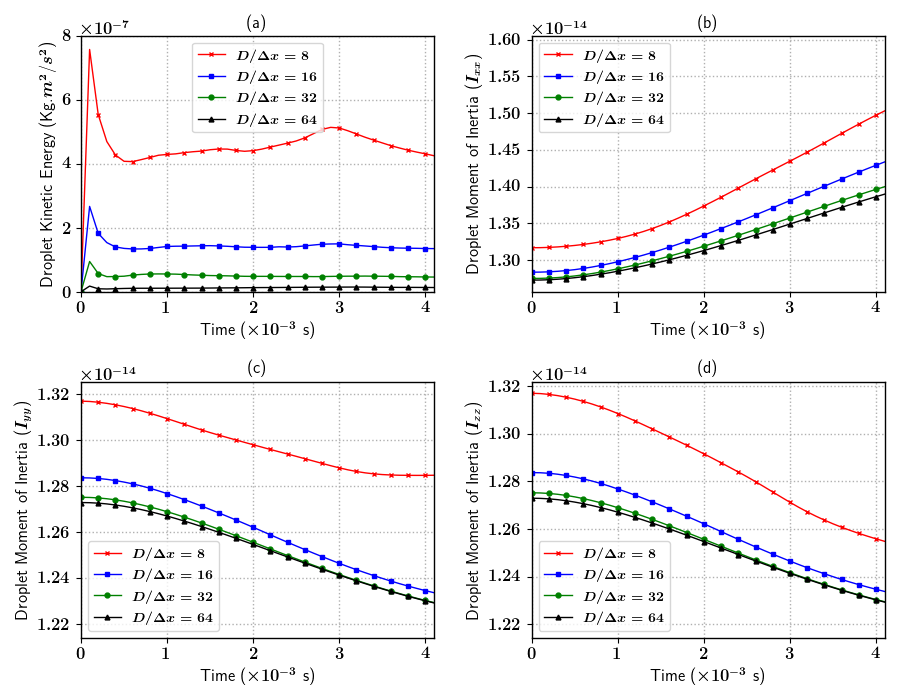
\includegraphics[width = 1.5\textwidth]{plots/raindrop/jcp_1.png}
\end{center}
\vspace*{-0.5cm}
\caption{Temporal evolution of quantities of interest to evaluate the 
	performance of our consistent scheme based on the 
	sub-grid (\textbf{MSUB}) method, for different spatial resolutions. 
	(a) Kinetic energy relative to the droplet center-of-mass as defined in \eqref{drop_ke}. 
	(b) Moment of inertia of the droplet along the flow (X) direction. 
	(c) and (d) Moment of inertia of the droplet along the directions 
	perpendicular to flow (Y,Z), evolution of $I_{yy}$ 
	seems to be more or less identical to $I_{zz}$.}
\label{multi_jcp}
\end{figure*}

% acc_conv caf_paper
\begin{figure}
\begin{center}
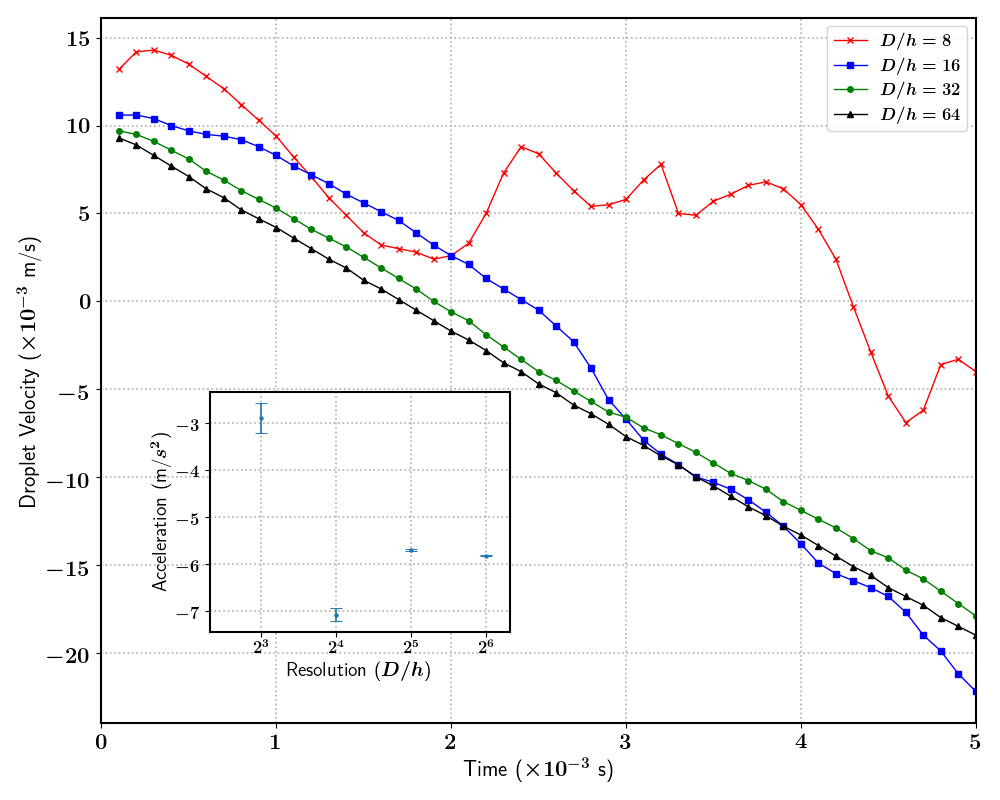
\includegraphics[width = 1.0\textwidth]{plots/raindrop/dropl_velocity_accel_ppd.png}
\end{center}
\vspace*{-0.5cm}
\caption{Comparison of droplet velocity as a function of time, for different droplet resolutions.
	The simulations were carried out with a consistent scheme based on the 
	shifted fractions (\textbf{MSHIFT}) method, using the WY advection scheme with the QUICK limiter. 
	The droplet velocities correspond to that of their respective center of masses. 
	Inset : Convergence of the droplet acceleration as a function of its resolution, 
	computed using the best linear fit over the temporal variation of their respective velocities. 
	The error bars signify the asymptotic standard error (least-squares) corresponding to the linear fits.} 
\label{drop_vel_caf}
\end{figure}

% acc_conv jcp_paper
\begin{figure}
\begin{center}
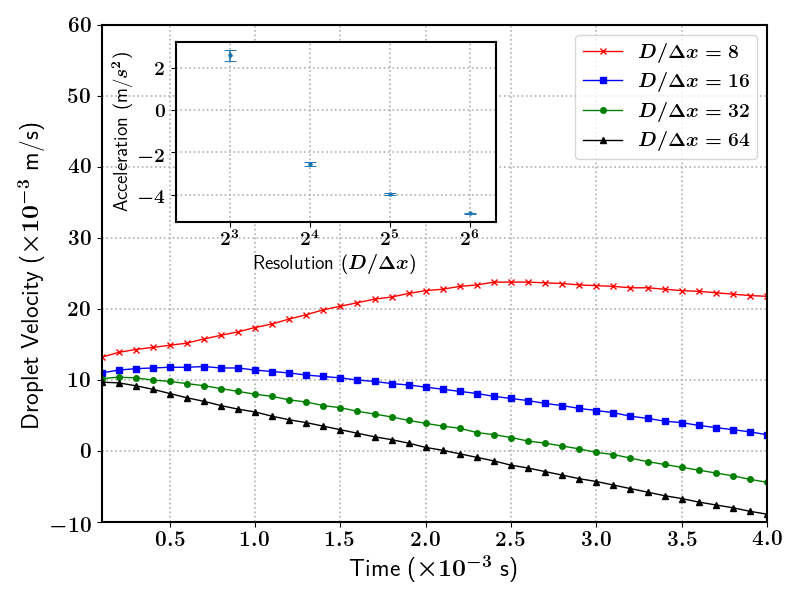
\includegraphics[width = 1.0\textwidth]{plots/raindrop/jcp_2.png}
\end{center}
\vspace*{-0.5cm}
\caption{Comparison of droplet velocity as a function of time, for different droplet resolutions.
	The simulations were carried out with a consistent scheme based on the 
	sub-grid (\textbf{MSUB}) method, using the WY advection scheme with the QUICK limiter. 
	The droplet velocities correspond to that of their respective center of masses. 
	Inset : Convergence of the droplet acceleration as a function of its resolution, 
	computed using the best linear fit over the temporal variation of their respective velocities. 
	The error bars signify the asymptotic standard error (least-squares) corresponding to the linear fits.} 
\label{drop_vel_jcp}
\end{figure}


\subsection*{Convergence Study}

For the next set of simulations, we use a fixed inflow velocity setup but with smaller initial velocity.
We systematically vary the resolution from  $D/h = 8, 16, 32 $ and $64$. 
Despite using our consistent methods, simulations at  $D/h = 8$ are sometimes unstable, 
so we use a workaround and use a lower fixed inflow velocity of $U_0=5$ m/s, 
which differs from the expected long term terminal velocity
$U_{t} \simeq $8 m/s used in the previous set of simulations. 
But, it does offer a milder initial condition and allows us to observe the first phase of the (physical)
acceleration towards the final statistical steady state. 
The simulations are carried out for 5 ms (for reasons of computational cost and also in order 
to avoid the droplet getting too close to the domain boundaries) 
and the convergence properties of the numerical system are examined within this time frame. 
A brief review of the relevant time scales are as follows : 

\begin{itemize}
\item The time scale $t_a=D/U_0$ of the air flow around the droplet, around 0.6 milliseconds, much shorter
than the simulation time. 
\item The time $t_w = L/[2(U_t - U_0)] = 3$ms that the droplet would take to travel by half the domain
  the domain once it had reached the terminal velocity. This time is not relevant here since one needs to wait first for the next two times
  before terminal velocity is reached. 
\item The time scale $t_c \simeq 15.1$ms \cite{rayleigh1879a} of capillary oscillations of the droplet shape.
\item The time scale $t_i$ of relaxation to terminal velocity. Using the dynamics \eqref{borda} below, 
	this time is $(\rho_l/\rho_g)\cdot( D/U_t) = 215 ms$, which is much longer than the simulation time. 
\item The time scale $t_\mu$ needed to entrain the internal vortical motion of the liquid under the action of the gas. An estimate this time is  $D^2/\nu_l =  \textrm{Re} D/U_t = 400 ms$.
\end{itemize}

The time of relaxation may be estimated using a simple square-velocity drag law for the droplet. 
We model the droplet motion as a one-dimensional dynamics under the effect of gravity and drag as

\begin{align}
	\rho_l \frac{\pi D^3}6 \frac{\textrm{d}U}{\textrm{d}t} =  \rho_l \frac{\pi D^3}6 g - C_D \rho_g \frac{\pi D^2} 8  U^2, \label{borda}
\end{align}

hence

\begin{align}
\frac{\textrm{d}U}{\textrm{d}t}  = -  \frac 34 \frac {r}{D} (U^2 - U_t^2) = -\frac{U-U_t}{t_i}, \label{dtu}
\end{align}

where for $U \simeq U_t$, thus giving us 

\begin{align}
t_i =  \frac 23 \frac {D}{r U_t}.
\end{align}

% mass conservation caf_paper
\begin{figure*}[h!]
\begin{center}
\begin{tabular}{cc}
\hspace*{-1.0cm}
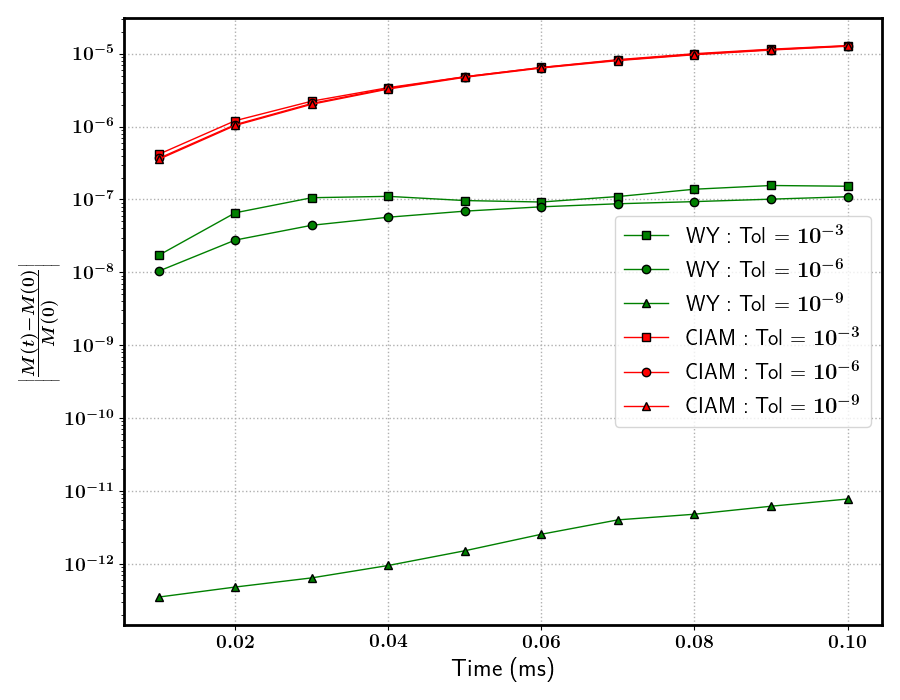
\includegraphics[width=0.7\textwidth]{plots/raindrop/raindrop_mass_conv_16ppd.png} & 
\hspace{-0.2cm}%
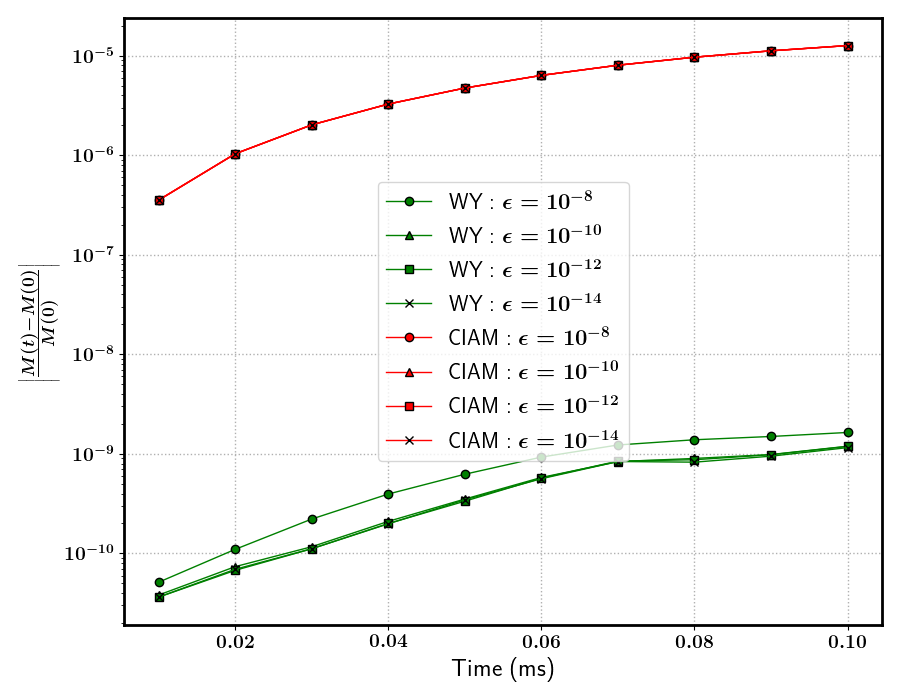
\includegraphics[width=0.7\textwidth]{plots/raindrop/raindrop_mass_conv_clipping.png} \\ 
\hspace{-0.2cm}%
(a) & (b) \\
\hspace*{-1.0cm}
\includegraphics[width=0.7\textwidth]{plots/raindrop/raindrop_mass_conv_resolution.png} & 
\hspace{-0.2cm}%
\includegraphics[width=0.7\textwidth]{plots/raindrop/new.png} \\ 
\hspace{-0.2cm}%
(c) & (d)
\end{tabular}
\end{center}
\caption{Relative change in the mass of the droplet 
as a function of time in plots (a), (b) and (c). 
The simulations are carried out with a resolution of $D/h = 16$, 
for a total time of $0.1$ milliseconds using the consistent 
scheme based on the shifted fractions (\textbf{MSHIFT}) method. 
The symbol ``WY'' in the legend corresponds to those run using 
the Weymouth-Yue advection scheme in combination with the QUICK limiter, 
and ``CIAM'' corresponds to the CIAM scheme in combination with the Superbee limiter. 
(a) Mass conservation properties of 
the scheme as a function of the Poisson solver tolerance is tested. 
For the WY-QUICK combination, using a stricter tolerance results 
in better mass conservation, whereas the conservation properties of the 
CIAM-Superbee combination seems to be independent of the tolerance.
(b) Dependence of the mass conservation on the clipping parameter ($\epsilon$) employed. 
The CIAM-Superbee combination again seems to be impervious to changes in clipping, 
whereas WY-QUICK seems to perform slightly better by lowering the parameter.
(c) Dependence of the mass conservation properties on the droplet resolution. 
The WY-QUICK combination displays better results for all except the lowest resolution.   
(d) Error estimation of the droplet acceleration in the frame of reference of the static box
	The corresponding accelerations are plotted in the inset of fig. \ref{drop_vel_caf}.}
\label{mass_conv}
\end{figure*}


We illustrate the performance of the consistent methods through the 
results of our simulations in figures \ref{multi_caf} and \ref{multi_jcp}
for the shifted fractions (\textbf{MSHIFT}) and sub-grid (\textbf{MSUB}) methods respectively. 
In case of both the methods, we use the WY advection scheme in combination with the QUICK flux limiter, 
while keeping the same value for the inflow velocity boundary condition. 
The quantities of interest while examining the robustness of the 
method are the temporal evolution of the droplet kinetic energy 
(figures \ref{multi_caf}. (a) and \ref{multi_jcp}. (a) ) 
and the moment of inertia of the droplet along the three directions 
(figures \ref{multi_caf}. (b),(c),(d) and \ref{multi_jcp}. (b),(c),(d)) . 
The inflow is along the X direction with gravity opposite to it. 
The moment of inertia is used as a descriptor of the 'average' droplet shape, 
with the three moments of inertia along the different axes $I_m$ defined as - 


\begin{align}
	I_m = \int_{\mathcal{D}} H x_m^2 d \boldsymbol{x} \quad , \quad \text{where}, \quad 1 \le m \le 3
\end{align}

where $\mathcal{D}$ is the computational domain and $x_m$ is the 
distance of the interface relative to the center of mass of the droplet.   
The droplet kinetic energy is defined relative to the droplet center-of-mass, given by 
 
\begin{align}
	E_k = \langle \rho(x,t) || \boldsymbol{u}(x,t) - \boldsymbol{u}_{CM}||^2 \rangle
	\label{drop_ke}
\end{align}

where $ \langle . \rangle$ is the spatial averaging operator over the  
entire domain and $\boldsymbol{u}_{CM}$ is the droplet center of mass.


The kinetic energy of the droplet evolves in a relatively smooth manner, 
without the presence of sudden spikes and falls which are emblematic of 
the standard non-consistent method (refer to Fig. \ref{pressure_2}). 
Such abrupt changes in kinetic energy of the droplet have been 
found to be associated with instants when the droplet undergoes 
`artificial' atomization or breakup, henceforth resulting in 
catastrophic loss of stability for the numerical method. 
We observe a systematic drop in the amount of the droplet 
kinetic energy as we increase resolution, with the most probable explanation 
being that of the suppression of spurious interfacial 
jitter which is rampant at lower resolutions. 
There is also a component of the kinetic energy of the droplet 
associated with the internal coherent vortical structures generated due to 
the interaction of aerodynamic shear at the interface, 
evidenced by the non-zero value of the kinetic 
energy even for the most highly resolved droplets. 
Finally, the moments of inertia of the droplet appear to evolve in a smooth manner 
for both our methods, for all droplet resolutions.

In figures \ref{drop_vel_caf} and \ref{drop_vel_jcp}, 
we show the velocity of the center of mass of the droplet 
(in the frame of reference of the box enclosing the droplet) 
as a function of time, and its behavior as we increase the droplet resolution. 
We have to keep in mind that the velocity inflow condition 
of $5$ m/s does not correspond to the terminal velocity 
field of an actual falling raindrop might experience, 
hence the droplet in our numerical setup has some 
near constant acceleration for very small times once the simulation are started.
The temporal variation in the droplet velocity is fitted to a 
linear polynomial in order to evaluate the droplet acceleration 
by means of a standard least-squares approach, for each droplet resolution. 
The observed accelerations (insets of figures \ref{drop_vel_caf} and \ref{drop_vel_jcp})
for the \textbf{MSHIFT} and \textbf{MSUB} methods are 
$\frac{\textrm{d}U}{\textrm{d}t} \simeq 5.8 \pm 0.1$ $m/s^2$
and $\frac{\textrm{d}U}{\textrm{d}t} \simeq 4.5 \pm 0.4$ $m/s^2$
respectively, the error estimates being obtained from the difference
between the $D/h = 2^5$ and the $D/h = 2^6$ resolutions.
The decrease of the error, obtained as above from the
difference between succesive resolutions using the \textbf{MSHIFT} method 
is plotted on Fig. \ref{mass_conv} (d), which shows the lack of any apparent 
order, although the second-order convergence line is plotted as a reference.

In Fig. \ref{mass_conv} we show the mass conservation properties 
of the shifted fractions method (\textbf{MSHIFT}) corresponding to the two most 
stable combinations, that is the WY advection with the QUICK 
flux limiter and the CIAM advection with the Superbee limiter. 
The mass conservation of the WY advection is strongly dependent
on how accurately the divergence-free condition is enforced, which
in turns is determined by the Poisson's solver tolerance. 
A clipping procedure, with no redistribution, affects mass conservation as well.
The WY combination is thus rather sensitive to these two parameters
but overall performs much better than the CIAM combination which is
inherently not mass-conserving and not very sensitive to the Poisson's solver 
tolerance and the clipping parameter $\epsilon$.
Mass conservation is also plotted with various 
resolutions $D/h$ in Fig. \ref{mass_conv}c. 
It is seen that going from $D/h=32$ to $D/h=64$
the mass variation becomes larger for both methods, and grows over time at 
high resolution for WY, pointing to an accumulation of many machine precision errors.

To sum it up, the results obtained in this chapter strongly suggest that 
our class of consistent numerical methods can be used to get relatively good 
estimates of the underlying flow features of the droplet without observing 
any un-physical evolution due to the discretization errors at low to moderate resolutions.           




\pagelayout{wide} % No margins
\addpart{Physics of Fragmentation}

\pagelayout{margin} % Restore margins
\setchapterpreamble[u]{\margintoc}

\chapter{Droplet Generation in Corrugated Ligaments}
\labch{breakup}


Ligaments constitute the penultimate stage in the complex sequence 
of capillary-driven topological changes that are 
typical of liquid fragmentation processes, 
finally resulting in the generation of polydisperse collections of drops. 
As we have seen in the previous chapter, there are several hypotheses 
in existing literature \sidecite{vill_1} 
that attempt to model the underlying physical mechanisms 
that are responsible for the selection of droplet size. 
A model first proposed by Villermaux and collaborators \sidecite{vill_2,vill_4}
asserts that the variance in the droplet sizes is strongly 
correlated to the initially corrugated shape of the 
ligament, from which the drops originate. 
These studies essentially demonstrate that the degree of polydispersity 
in the drop sizes can quite simply, be explained by considering the 
geometric shape of the ligaments, irrepective of the sequence of 
complicated fragmentation processes that gave rise to them in the first place.  


\begin{marginfigure}[4cm]
\centering
\includegraphics{plots/ligament_breakup/lig_mar_vill_pof04.png}
\caption{Fragmentation of stretched liquid (Newtonian) ligaments, reproduced 
	from Marmottant \& Villermaux \cite{vill_3}.
       	The complex rearrangement of the liquid volumes 
	inside the ligament results in its disintegration 
	into droplet of various sizes. 
	}
\end{marginfigure}

\marginnote{
The corrugation-coalescence mechanisn has been 
popularized in several studies such as \cite{vill_3,vill_1,vill_5,vill_6,vill_7},
and more recently in \cite{bonn,mckinley}.
}

In the context of the present body of work, we shall 
only concern ourselves with the dynamics of Newtonian fluids, 
described by the Navier-Stokes equations at the incompressible
and isothermal limits. 
The rearrangement of the liquid volumes that constitute
the ligaments play a key role in determining the size 
of the droplets that emerge immediately after the disintegration
of the ligament structure.  
The dynamics of these rearrangements prior to breakup are 
governed by non-linear interactions between several 
physical mechanisms such as the propagation of capillary waves
along the ligament surface, remnants of the internal flow, 
stretching induced by either the surrounding 
gas flow or acceleration into the surrounding medium itself,
and the dissipative effects of viscosity.  


%Due to the complex nature of such fragmentation processes, 
%it has proven to be quite a difficult challenge for both 
%experimental and numerical studies to establish the 
%mechanistic link between the initial surface corrugations 
%and the resulting drop size distributions.  
%
%
%In the present study, we have developed a numerical experiment 
%that grants us precise control over both quantitative and 
%qualitative aspects of such random corrugations, and its subsequent 
%influence on the resulting droplet sizes. 



\section{Breakup Regimes}

% Brief review, eggers , Keller-Miksis and Viscous regimes


%---------------------------------------------------------------
\section{Numerical Setup}
We perform direct numerical simulations of the two-phase 
Navier-Stokes equations under the incompressible framework. 
Material properties correspond to that of air-water systems at 20 degrees Celsius. 
Simulations are carried out in the axi-symmetric framework, 
therefore excluding the existence of azimuthal modes with 
respect to the central axis of the ligament. 

\paragraph{Platform : Basilisk}
\blindtext

\paragraph{Computational Schematic}
\blindtext

\paragraph{Random Surface Generation}
\blindtext

\paragraph{Parameterization}
\blindtext

\paragraph{Quantization of Waves}
\blindtext

%---------------------------------------------------------------

\section{Impact of Initial Conditions}

\paragraph{3D vs. 2D Simulations}
\blindtext

\paragraph{Effect of Spatial Resolution}
\blindtext

\paragraph{Effect of Droplet Removal}
\blindtext

\paragraph{Effect of Corrugation Amplitude}
\blindtext

\paragraph{Effect of Ohnesorge Number}
\blindtext

\paragraph{Effect of Cut-Off Wavenumber}
\blindtext

\paragraph{Effect of Aspect Ratio}
\blindtext



\setchapterpreamble[u]{\margintoc}
\chapter{Statistical Approach to Drop Formation}
\labch{dropstat}


\section{Monte Carlo Approach}



% determination of droplet diameter and volume 



\section{Millimeter Scale Ensembles}

We turn our attention towards slender ligaments whose widths are of the 
order of millimeters, a scale at which a multitude of fragmentation phenomena
\sidenote{Some examples of fragmentation at this length scale involve ligaments
generated by drop splashes on different substrates, secondary atomization of raindrops etc. 
}
take place, that are more or less visible to the naked eye.
In particular, for air-water systems (20 degree Celsius) the millimeter length 
scale corresponds to $Oh \sim O(10^{-2})$, where $Oh$ is the Ohnesorge number
based on the characteristic length scale of the ligaments. 
The characterization of our corrugated ligament setup using the set of adimensional
(e.g. \eqref{base_params}) numbers as discussed in the previous chapter is extended 
to describe our ensemble of ligaments, such that the exact set of parameters
correspond to a unique point in the phase space $\Phi$ of all possible combinations. 
The coalescences that intermittently occur after the initial breakup phase of 
the thread-like structure not only change the number of drops, but also impact the 
mean and dispersion of the size distribution due to the increase in the number of drops that 
are significantly larger than the width of the ligament of origin.   
This aspect of temporal dependence of the drop sizes corresponding to a particular ligament ensemble
is taken into account by specifying the time at which the statistics are recorded. 
Thus, our droplet ensembles associated with the millimeter scale ligaments can be uniquely described 
by a combination of the time $T$ and $\Phi_0$, where

\begin{align}
	\Phi_0 \equiv \left( Oh=10^{-2}, K=2\pi, \epsilon=1.0, \Lambda=50 \right). 
\end{align}

The definitions of the adimensional groups are identical to that used
in the previous chapter, hence are not repeated.
Statistical descriptions of the drop sizes are commonly carried out using
particular probability density functions (PDF) defined as follows 



\begin{align}
	\text{Gaussian : } \quad P\left( x ; \mu , \sigma \right) &= 
	\frac{1}{\sigma \sqrt{2\pi}} \textrm{exp}\left[-\frac{1}{2}\left(\frac{x - \mu}{\sigma}\right)^2\right] \label{gauss},\\
	\text{Log-Normal : } \quad P\left( x ; \mu , \sigma \right) &= 
	\frac{1}{x \sigma \sqrt{2\pi}} \textrm{exp}\left[-\frac{1}{2}\left(\frac{\log x - \mu}{\sigma}\right)^2\right] \label{log_normal},\\
	\text{Gamma : } \quad P\left( x ; n,k \right) &= 
	\frac{k^{n}}{\Gamma(n)} x^{n-1} \textrm{exp}\left(-k x\right) \label{gamma}, 
\end{align}

where $x$ is the variable (diameter, volume etc) in question. 
The Gamma distribution can be rearranged so that $x$ represents
the variable rescaled by its mean ($n / k$), which becomes 

\begin{align}
	P\left( x ; n \right) = \frac{n^{n}}{\Gamma(n)} x^{n-1} \textrm{exp}\left(-n x\right) . 
\end{align}

The rescaling of variable results renders the function dependent solely 
on the parameter $n$, identical to the form first used in \cite{vill_2}
to represent the distribution of the normalized diameter.  
At the large size limit of the distributions, the leading order terms 
scale as $P(x) \sim \textrm{exp}(-x^2)$ for the Gaussian, $P(x) \sim \textrm{exp}(- \log x)$ for 
the Log-Normal and finally $P(x) \sim \textrm{exp}(- x)$ in case of the Gamma function. 
In essence, out of the three density functions, the Guassian predicts the lowest frequency of
rare events (very large drops), the Log-Normal predicts the highest frequency whereas
the Gamma function prediction is somewhere in between the other two. 

\begin{marginfigure}[-1cm]
\centering
\includegraphics{plots/drop_stats/diameter_compute.pdf}
\caption{The shaded area $A$ represented by the dotted and dashed lines
	is used to estimate the diameter of the droplet in question.
	The resulting diameter is computed as $D = \sqrt{4A/\pi}$,
	and the corresponding volume is given by $V = \pi D^3/6$.
	} 
\label{dia_compute}
\end{marginfigure}

Another important aspect to consider is the bin-width of the 
histograms used to construct the probability distributions. 
There are several choices regarding the criteria used to determine the optimal bin-width, 
taking into consideration the size, variability and skewness of the underlying data set. 
In in interest of simplicity, we restrict our focus to histograms with uniform bin-width. 
In order to ascertain the dependence (if any) of the distribution on the number of bins  
(uniform size), we use $4$ different estimators, the open source implementations of which
can be found in the Numpy library \cite{numpy}.
The simplest of the four estimators selects the number 
of bins as the square root of the sample size.
Another estimator is also based solely on the size of the dataset, 
but the number of bins scales as the cube root of the data size.  
A more robust estimator that takes into account the variability in the dataset
is the Freedman Diaconis estimator, in which the bin width is proportional to the 
inter quartile range, and inversely proportional to the cube root of the data size. 
Finally, we also use an improved version of the Sturges estimator, that performs 
well for non-normal datasets due to the fact that it takes into account the skewness. 

In the subsequent sections, we present a statistical picture of the drop sizes generated 
from our ligament ensemble $\Phi_0$, where the sample size is of the order of $64,000$.
The droplet data is primarily recorded on slow time scales, so that the data reflects 
a considerable amount of coalescences after the initial destabilization of the ligaments. 
In order to extract the diameter and volumes of the drops generated in our axisymmetric
simulations, we for the commonly used area based estimation (see Fig. \ref{dia_compute}).


\subsection*{Diameter Distributions}

Figures \ref{t1_dia_bins} and \ref{t2_dia_bins} illustrate the probability distributions
of the normalized droplet diameter corresponding to $T=15$ and $T=30$ respectively. 
The diamters are normalized using the means of the associated samples. 
The bin widths are always based on the properties of the largest sample.
As one can observe, there are fewer drops in the largest sample at $T=30$ 
compared to the largest sample at $T=30$, due to the additional coalescences.  
The drop diameters are found to be more or less symmetrically distributed about the mean,
although there is an small peak at the lower end of the dis.
The choice of binning criteria does not seem to have any noticable effect on the 
overall shape of the distribution, regardless of the size of the sample $N$.   
A Guassian probability density function \eqref{gauss} appears to be a good 
approximation to the underlying distribution.
It is important to note that the Gaussian curve is not fitted to the heights of the 
histogram bins, instead it is plotted on top of the distributions using the mean and 
variance corresponding to the largest sample size, therefore rendering it independent
of the choice of bin-width and free from any additional fitting parameters.  


\begin{figure*}
\centering
\includegraphics{plots/drop_stats/short_time_diameter_bins.pdf}
\caption{Probability distribution functions of the droplet diameter at time $T = 15$. 
The ensemble is characterized by $\Phi_0 \equiv \left( Oh = 10^{-2}, K = 2\pi , \varepsilon = 1.0 , \Lambda = 50 \right)$. 
The diameters are normalized by the mean of the corresponding sample.  
The distributions are generated using datasets corresponding to four different sample sizes, 
including four different choices of (uniform) bin width. 
The Gaussian functions are characterized by the mean and variance of the original dataset, 
hence they are plotted alongside the histograms instead of being fitted to the bin heights.
	}
\label{t1_dia_bins}
\end{figure*}

% long time scales



\begin{figure*}
\centering
\includegraphics{plots/drop_stats/long_time_diameter_bins.pdf}
\caption{Probability distribution functions of the droplet diameter at time $T = 30$. 
The ensemble is characterized by $\Phi_0 \equiv \left( Oh = 10^{-2}, K = 2\pi , \varepsilon = 1.0 , \Lambda = 50 \right)$. 
The diameters are normalized by the mean of the corresponding sample.  
The distributions are generated using datasets corresponding to four different sample sizes, 
including four different choices of (uniform) bin width. 
The Gaussian functions are characterized by the mean and variance of the original dataset, 
hence they are plotted alongside the histograms instead of being fitted to the bin heights.
	}
\label{t2_dia_bins}
\end{figure*}

% PDF predictions of data at long times


\begin{figure*}
\centering
\includegraphics{plots/drop_stats/long_time_diameter_fits.pdf}
\caption{Probability distribution functions of the droplet diameter at time $T = 30$. 
The ensemble is characterized by $\Phi_0 \equiv \left( Oh = 10^{-2}, K = 2\pi , \varepsilon = 1.0 , \Lambda = 50 \right)$. 
The diameters are normalized by the mean of the corresponding sample.  
The distribution is generated using 81 bins of uniform size, represented in green.  
The Gaussian and Log-Normal functions are characterized by the mean and variance of the original dataset, 
therefore are plotted alongside the histogram, whereas, the Gamma function is fitted to the bin heights,
with $n= 11.63$ being the value corresponding to the best fit.
	}
\label{t2_dia_fits}
\end{figure*}

% N^{-1/2} scaling of error 

In Fig. \ref{t2_dia_fits}, we present a comparison of the different probaility 
density functions applied to the largest ensemble of drops characterized by $\Phi_0$ and $T=30$. 
The Gaussian is found to be the best approximation to the normalized 
diameter distribution, followed by the Gamma and Log-Normal functions.
The Gaussian and Log-Normal curves are generated using the mean and variance 
of the dataset, whereas the free parameter $n$ of the Gamma function is determined
according to the best least-squares fit over the histogram. 
A noteworthy point demonstrated by the inset of Fig. \ref{t2_dia_fits} is that
the error \sidenote{The error is defined as the $L_2$ norm of the differences 
between the bin hights of the sample and the largest sample, where both 
samples have identical bin-width.} scales as $N^{-1/2}$, $N$ being the sample size.
Additionally, the scaling is not sensitive to the choice of bin-width. 
This strongly suggests the absence of any unforeseen correlations between the 
individual realizations (corrugated ligaments) that form the ensemble.


\subsection*{Volume Distributions}

We now shift our attention towards the distribution of droplet volumes. 
Figures \ref{t1_vol_bins} and \ref{t2_vol_bins} show the PDFs 
of the normalized droplet volume corresponding to $T=15$ and $T=30$ respectively. 
The volumes are normalized by the means of the associated samples. 
As in the diameter distributions, the bin widths are always 
based on the properties of the largest sample.
In stark contrast to the case of the diameters, the drop volumes
are found to be heavily skewed towards the smaller sizes.
Similar to the diameter PDFs, the choice of bin-width seems to not have any considerable impact
on the overall shape of the distribution, and is also independent of the sample size.   
In this case though, the single parameter Gamma density function \eqref{gamma} appears to
be the approximation to the volume distribution, with the best fit corresponding to 
values of $n \approx 1.68$ and $n \approx 1.58$ corresponding to $T=15$ and $T=30$ respectively.
There is a slight dependence of the parameter $n$ on the bin-width, which is expected 
as $n$ itself is determined according to the best fit to the histogram in question.

% short time scale 

\begin{figure*}
\centering
\includegraphics{plots/drop_stats/short_time_volume_bins.pdf}
\caption{Probability distribution functions of the droplet volume at time $T = 15$. 
The ensemble is characterized by $\Phi_0 \equiv \left( Oh = 10^{-2}, K = 2\pi , \varepsilon = 1.0 , \Lambda = 50 \right)$. 
The volumes are normalized by the mean of the corresponding sample.  
The distributions are generated using datasets corresponding to four different sample sizes, 
including four different choices of (uniform) bin width. 
The Gamma functions are characterized by the parameter $n$, the value of which is determined 
by that which provides the best (least-squares) fit to the corresponding bin heights.  
	}
\label{t1_vol_bins}
\end{figure*}

% long time scale

\begin{figure*}
\centering
\includegraphics{plots/drop_stats/long_time_volume_bins.pdf}
\caption{Probability distribution functions of the droplet volume at time $T = 30$. 
The ensemble is characterized by $\Phi_0 \equiv \left( Oh = 10^{-2}, K = 2\pi , \varepsilon = 1.0 , \Lambda = 50 \right)$. 
The volumes are normalized by the mean of the corresponding sample.  
The distributions are generated using datasets corresponding to four different sample sizes, 
including four different choices of (uniform) bin width. 
The Gamma functions are characterized by the parameter $n$, the value of which is determined 
by that which provides the best (least-squares) fit to the corresponding bin heights.  
	}
\label{t2_vol_bins}
\end{figure*}

Fig. \ref{t2_vol_fits} shows a comparison of the different probaility 
density functions applied to the largest ensemble of drops characterized by $\Phi_0$ and $T=30$. 
The Gamma density function is found to be the best approximation to the normalized 
volume distribution, followed by the Log-Normal and Gaussian functions.
Similar to the diameter case, the Gaussian and Log-Normal curves are 
generated using the mean and variance of the dataset, 
whereas the free parameter $n$ of the Gamma function is determined
according to the best least-squares fit over the histogram. 
As seen before, the error (inset of Fig. \ref{t2_vol_fits}) 
scales as $N^{-1/2}$, regardless of the binning criteria used. 

% PDF predictions of data at long times

\begin{figure*}
\centering
\includegraphics{plots/drop_stats/long_time_volume_fits.pdf}
\caption{Probability distribution functions of the droplet volume at time $T = 30$. 
The ensemble is characterized by $\Phi_0 \equiv \left( Oh = 10^{-2}, K = 2\pi , \varepsilon = 1.0 , \Lambda = 50 \right)$. 
The diameters are normalized by the mean of the corresponding sample.  
The distribution is generated using 108 bins of uniform size, represented in green.  
The Gaussian and Log-Normal functions are characterized by the mean and variance of the original dataset, 
therefore are plotted alongside the histogram, whereas, the Gamma function is fitted to the bin heights,
with $n= 1.57$ being the value corresponding to the best fit.
	}
\label{t2_vol_fits}
\end{figure*}

% N^{-1/2} scaling of error 


\subsection*{Influence of Corrugation Amplitude}

\begin{marginfigure}[2cm]
\centering
\includegraphics{plots/drop_stats/amp_long_compare.pdf}
	\caption{The fate of two ligaments whose initial surfaces 
	are created using the same set of random overlapping waves, 
	but differ by the strength of the perturbations.
	The ligament on the left is part of ensemble $\Phi_1$ 
	and the one on the right is part of $\Phi_2$. 
	The droplets enclosed in the boxes (dashed lines)
	are characteristic of the distintegration of weakly perturbed ligaments,
	wherein their sizes are smaller than the typical size at least by a factor of $2$. 
	}
\label{amp_long_comp}
\end{marginfigure}

As discussed in the previous chapter, the ``smoothness'' of the initial geometrical
shape of the ligament is expected to have a significant influence on the 
destabilization of the liquid thread and the concomitant coalescence dynamics.
In order to ascertain the impact of the strength of the initial perturbations
on the resulting drop size distribution, we conduct simulations of two different 
millimeter scale ensembles $\Phi_1$ and $\Phi_2$. Both of them are characterized 
by the same set of adimensional parameters as in $\Phi_0$, except that $\varepsilon = 0.4$
in case of $\Phi_1$, whereas $\varepsilon = 1.6$ in case of $\Phi_2$.

For the case of weakly perturbed ligaments, Fig. \ref{tseries_small} 
demonstrates the temporal evolution of the droplet diameter distributions, 
where the diameter is rescaled by the (mean) width $W$ of the initial ligaments. 
At small time scales, the distribution is bimodal in nature, consisting of a large
number of drops that are quite smaller than even the initial ligament width. 
This may be a consequence of the non-linear effects \cite{satellite_1,satellite_2} 
that kick in immediately following the initial linear (exponential) growth phase, 
often resulting in the liquid thread disintegrating into a collection of main 
and (significantly smaller) satellite drops (see Fig. \ref{amp_comp} in the preceding chapter). 
At large times, the peak corresponding to the smaller sizes is considerably diminished, 
whereas the larger size peak develops into more of a ``plateau'' type shape.  
This observed shifts in the distribution as a function of time can be explained by the 
successive coalescences taking place, where the smallest drops coalesce with the largest drops.
By largest drops, we mean the ones situated to the right of the large size peak, 
corresponding to the region of the distribution which eventually gives rise to the plateau shape.


Coming to the strongly perturbed ligament shapes, Fig. \ref{tseries_large} illustrates 
the unimodal character of the overall distribution shape.
There seems to be a lack of any significant qualitative change 
when comparing the distributions at small and large time scales. 
The large amplitude perturbations of the ligament surface do not 
allow for any significant amount of liquid rearrangement within the bulk prior 
to disintegration, thus the collection of drops formed immediately following the breakup
of the thread-like structure are quite disperse when with respect to their sizes.
The mean of the distribution displays a slight shift towards the larger sizes, with the passage of time. 
This shift can be explained by the effect of random coalescences amongst droplets corresponding to all sizes.

To summarize, in Fig. \ref{tseries_comp} we present a side-by-side comparison of 
the aforementioned temporal evolutions of the droplet diameter distributions.  
We infer that the primary influence of the corrugation strength 
is that it changes the nature of the resulting distribution from bimodal to unimodal,
as one increases the amplitude of the initial perturbations. 
Although the dynamics of the droplet coalescences (post-breakup) follow different trajectories
in accordance with the corrugation strength (see Fig. \ref{amp_long_comp}), 
the distributions at large times end up looking rather similar.

% temporal variation in drop size PDF's for low and high levels of corrugation

\begin{figure}
\centering
\includegraphics{plots/drop_stats/small_amp.pdf}
\caption{Temporal evolution of the probability distribution functions of the droplet diameter.
	The diameter is rescaled by the initial width $W$ of the ligaments.
	The ensemble is characterized by $\Phi_1 \equiv \left( Oh = 10^{-2}, K = 2\pi 
, \varepsilon = 0.4 , \Lambda = 50 \right)$, thus consisting of \textit{weakly} perturbed 
initial ligaments shapes. 
	}
\label{tseries_small}
\end{figure}

\begin{figure}
\centering
\includegraphics{plots/drop_stats/large_amp.pdf}
\caption{Temporal evolution of the probability distribution functions of the droplet diameter.
	The diameter is rescaled by the initial width $W$ of the ligaments.
	The ensemble is characterized by $\Phi_2 \equiv \left( Oh = 10^{-2}, K = 2\pi 
, \varepsilon = 1.6 , \Lambda = 50 \right)$, thus consisting of \textit{strongly} perturbed 
initial ligaments shapes. 
	}
\label{tseries_large}
\end{figure}

% side by side comparison
% extrapolations of RP etc , limit of volume of largest drop


\begin{figure*}
\centering
\includegraphics{plots/drop_stats/amp_dist_compare.pdf}
\caption{Comparison between the temporal evolution of the probability distribution functions of the
	droplet diameter, corresponding to the strongly ($\varepsilon = 0.4$) and 
	weakly ($\varepsilon = 1.6$) perturbed ligament ensembles. 
	The diameter is rescaled by the width of the initial ligament. 
	The ensembles are characterized by $\Phi_{\{1,2\}} \equiv \left( Oh = 10^{-2}, K = 2\pi 
, \varepsilon = \{0.4,1.6 \} , \Lambda = 50 \right)$. 
The thick dashed lines correspond to the mean of the respective distribution, and the thinner
dashed lines located on both sides of the thicker line corresponding to the respective interquartile ranges. 
	}
\label{tseries_comp}
\end{figure*}


\section{Description of Large Sizes}


% estimation of error with binomial distribution



% linear fitting, with and without uncertainty, full distribution and tail zoom  

% methodology to determine best fit

\begin{figure}
\centering
	\includegraphics{plots/drop_stats/determine_fit_linear.pdf}
	\caption{\blindtext}
\label{determine_linear}
\end{figure}


% without uncertainty

\begin{figure}
\centering
\includegraphics{plots/drop_stats/linear_tail_fit_uncertainty_no.pdf} \\
\includegraphics{plots/drop_stats/linear_zoom_tail_fit_uncertainty_no.pdf} \\ 
\caption{\blindtext}
\label{linear_fits_wo}
\end{figure}

% with uncertainty

\begin{figure}
\centering
\includegraphics{plots/drop_stats/linear_tail_fit_uncertainty_yes.pdf} \\
\includegraphics{plots/drop_stats/linear_zoom_tail_fit_uncertainty_yes.pdf} \\ 
\caption{\blindtext}
\label{linear_fits_with}
\end{figure}


% log(log) vs log fitting, with and without uncertainty, full distribution and tail zoom  

% methodology to determine best fit

\begin{figure}
\centering
	\includegraphics{plots/drop_stats/determine_fit_log.pdf}
	\caption{\blindtext}
\label{determine_log}
\end{figure}

% without uncertainty

\begin{figure}
\centering
\includegraphics{plots/drop_stats/log_tail_fit_uncertainty_no.pdf} \\
\includegraphics{plots/drop_stats/log_zoom_tail_fit_uncertainty_no.pdf} \\ 
\caption{\blindtext}
\label{log_fits_wo}
\end{figure}


% with uncertainty

\begin{figure}
\centering
\includegraphics{plots/drop_stats/log_tail_fit_uncertainty_yes.pdf} \\
\includegraphics{plots/drop_stats/log_zoom_tail_fit_uncertainty_yes.pdf} \\ 
\caption{\blindtext}
\label{log_fits_with}
\end{figure}

\subsection*{Weakly Non-Linear Theory}



% stephane's predictions and verifications




\pagelayout{wide} % No margins
\setchapterpreamble[u]{\margintoc}
\chapter{Conclusions \& Perspectives}
\labch{conclusion}

In this thesis, numerical investigations pertaining to two different aspects 
of liquid-gas interfacial flows with marked density contrasts were conducted 
using advanced geometrical reconstruction based Volume-of-Fluid methods. 
The first aspect involved understanding and eventually suppressing certain types of 
instabilities that plague standard numerical models due to the cascading growth of
discretization errors that are particularly rampant at low to moderate numerical resolution.  
On the other hand, the second aspect of the investigation deals with a statistical description
of drop sizes, where the drops were generated by carrying out large ensembles of well resolved 
direct numerical simulations of the capillary-induced breakup of randomly corrugated ligaments. 

In the first part of the thesis, a detailed exposition into the design and 
development of our numerical methods is provided, where the principle 
of maintaining consistency between the discrete transport of
the discontinuous mass and momentum fields were implemented  
using a conservative discretization of the two phase 
Navier-Stokes equations on staggered Cartesian grids. 
The \textit{shifted fractions} and \textit{sub-grid} methods were developed
specifically in order to address the challenge of consistent 
advection of volume fraction, mass and momentum on staggered grids,
coupled with the extension of the conservative direction-split mass transport
algorithm of Weymouth and Yue \cite{wy} to the direction-split transport of momentum.
Several performance aspects of the aforementioned methods were presented using 
standard benchmark cases such as the behavior of spurious currents in static and
moving droplets, and the propagation of damped capillary waves. 
Each of these tests were conducted for density contrasts spanning several orders of magnitude, 
including a realistic air-water configuration for the case of capillary waves. 
Both of our consistent methods demonstrate slight to moderate levels of increased accuracy
when compared to the standard version of our method that is not 
consistent with respect to mass-momentum transport. 
A second-order error convergence rate is observed in the case of the 
static droplet and the capillary wave, with the rate
reverting to first-order in the case of droplet advection.
Finally, the robustness and stability of the present method was demonstrated
using the case of a raindrop falling in air, which involves complex interactions
of capillary forces, viscosity and inertia combined with the difficulties associated
with flows involving marked density contrasts.  
A key feature of the our class of consistent methods is the ability to circumvent 
or suppress the un-physical interfacial deformations that are rampant 
in the case of the standard non-consistent method, which typically results in the 
``artificial'' atomization of the raindrop .
Our methods are able to deliver relatively good estimates of the flow features 
especially at low to moderate resolutions, as evidenced by the smooth evolution 
of the droplet kinetic energy and the moments of inertia describing the average shape. 
Furthermore, both methods are able to reproduce the physically consistent early phase 
(almost constant) acceleration of the droplet towards the final statistical steady state.  

Many of the complications in our methods are due to the staggered arrangement of the primary variables, 
thus opening a possible avenue for exploration of different grid configurations when it comes to consistent transport.
Another perspective is an assessment of the computational speed-up 
of our methods compared to standard non-consistent methods which necessitate 
significantly higher spatial resolutions in order to ensure numerical stability.  
An interesting possibility exists in the context of the \textit{sub-grid} method, 
where volume fraction information from the doubly refined grid could be used to
obtain more accurate estimations of the interface curvature defined on the coarse grid level. 
An interesting test would be to verify if both the consistent and non-consistent methods
converge to identical solutions at sufficiently large mesh resolution, owing to the fact that they 
are based on identical governing equations and differ mainly due to the choice of discretization scheme. 


Moving onto the second part of the thesis, a thorough description of the 
methodology behind the generation of slender periodic ligaments is provided, 
where the ligament surfaces are created via superposition of random overlapping waves.
A numerical setup was developed that enables precise quantitative control over the 
statistical properties of the randomly corrugated initial surface profiles, 
therefore setting up the stage for obtaining controllable, reliable and reproducible 
ensembles of droplets that are generated via disintegration of the original ligaments.
High fidelity simulations of ligaments corresponding to air-water systems were carried out,
delineating the influence of important factors such as the length scale, time scale, 
aspect ratio and strength of the initial corrugations on the subsequent set of drops formed.  
In the case of moderately perturbed millimeter scale water ligaments in air, 
the diameters of the resulting drops were found to be (approximately) symmetrically 
distributed around the mean size, where the overall shape is relatively well described by 
a Gaussian probability density function devoid of any free parameters.
The shape of the diameter distributions are fairly robust, displaying negligible sensitivity
to the choice of bin-width used to generate the histograms.
In addition, the distributions converge towards a fixed shape as we increase the sample size $N$, 
where the error (defined with respect to the largest sample) scales as $N^{-1/2}$, therefore strongly 
suggesting the absence of any hidden correlations between the individual realizations consituting the sample. 
Amongst the initial conditions that influence the shape of the diameter distribution, the strength of 
the corrugations act as a bifurcation parameter, changing the bimodal nature of the distribution shape for 
weakly perturbed ligaments to a unimodal one as we go towards stronger initial perturbations. 
Interestingly in the case of moderately perturbed ligaments, the tail of the diameter 
distribution corresponding to the large drops are best described by an exponential scaling of
the form $e^{-d^6}$ even though the overall distribution seems to scale as $e^{-d^2}$. 
This scaling result was found to be independent of whether uncertainty in the bin heights
were included or not, and further verified by reconstructing the histograms on "$\log(\log)$ vs. $\log$" scales.      
Finally, a Gaussian random process theory for near-monochromatic waves was developed 
in an effort to explain the origins of the newfound $e^{-d^6}$ scaling.
In the surface tension dominated regime associated to weakly perturbed initial ligament shapes, 
the theory predicts a resulting drop diameter distribution in the form of a $d^3$- Gaussian, 
as well as a functional relationship between the dispersion in the size of the drops and the 
variance of the initial pertubations used to create the corrugated ligament surface. 
The theoretical predictions significantly differ from the observations derived from our numerical experiments
corresponding to \textit{moderately} perturbed ligament shapes, therefore opening the perspective
of verifying the predictions within its scope of validity i.e. adequately large ensembles of \textit{weakly} perturbed ligaments.


    



%\pagelayout{wide} % No margins
%\addpart{s}
%\pagelayout{margin} % Restore margins

%\appendix % From here onwards, chapters are numbered with letters, as is the appendix convention
%
%\pagelayout{wide} % No margins
%\addpart{Appendix}
%\pagelayout{margin} % Restore margins

%\setchapterstyle{lines}
\labpage{appendix}
\blinddocument


%----------------------------------------------------------------------------------------

\backmatter % Denotes the end of the main document content
\setchapterstyle{plain} % Output plain chapters from this point onwards

%----------------------------------------------------------------------------------------
%	BIBLIOGRAPHY
%----------------------------------------------------------------------------------------

% The bibliography needs to be compiled with biber using your LaTeX editor, or on the command line with 'biber main' from the template directory

\defbibnote{bibnote}{Here are the references in citation order.\par\bigskip} % Prepend this text to the bibliography
\printbibliography[heading=bibintoc, title=Bibliography, prenote=bibnote] % Add the bibliography heading to the ToC, set the title of the bibliography and output the bibliography note

%----------------------------------------------------------------------------------------
%	NOMENCLATURE
%----------------------------------------------------------------------------------------

% The nomenclature needs to be compiled on the command line with 'makeindex main.nlo -s nomencl.ist -o main.nls' from the template directory

%\nomenclature{$c$}{Speed of light in a vacuum inertial frame}
%\nomenclature{$h$}{Planck constant}
%
%\renewcommand{\nomname}{Notation} % Rename the default 'Nomenclature'
%\renewcommand{\nompreamble}{The next list describes several symbols that will be later used within the body of the document.} % Prepend this text to the nomenclature
%
%\printnomenclature % Output the nomenclature

%----------------------------------------------------------------------------------------
%	GREEK ALPHABET
% 	Originally from https://gitlab.com/jim.hefferon/linear-algebra
%----------------------------------------------------------------------------------------

%\vspace{1cm}
%
%{\usekomafont{chapter}Greek Letters with Pronounciation} \\[2ex]
%\begin{center}
%	\newcommand{\pronounced}[1]{\hspace*{.2em}\small\textit{#1}}
%	\begin{tabular}{l l @{\hspace*{3em}} l l}
%		\toprule
%		Character & Name & Character & Name \\ 
%		\midrule
%		$\alpha$ & alpha \pronounced{AL-fuh} & $\nu$ & nu \pronounced{NEW} \\
%		$\beta$ & beta \pronounced{BAY-tuh} & $\xi$, $\Xi$ & xi \pronounced{KSIGH} \\ 
%		$\gamma$, $\Gamma$ & gamma \pronounced{GAM-muh} & o & omicron \pronounced{OM-uh-CRON} \\
%		$\delta$, $\Delta$ & delta \pronounced{DEL-tuh} & $\pi$, $\Pi$ & pi \pronounced{PIE} \\
%		$\epsilon$ & epsilon \pronounced{EP-suh-lon} & $\rho$ & rho \pronounced{ROW} \\
%		$\zeta$ & zeta \pronounced{ZAY-tuh} & $\sigma$, $\Sigma$ & sigma \pronounced{SIG-muh} \\
%		$\eta$ & eta \pronounced{AY-tuh} & $\tau$ & tau \pronounced{TOW (as in cow)} \\
%		$\theta$, $\Theta$ & theta \pronounced{THAY-tuh} & $\upsilon$, $\Upsilon$ & upsilon \pronounced{OOP-suh-LON} \\
%		$\iota$ & iota \pronounced{eye-OH-tuh} & $\phi$, $\Phi$ & phi \pronounced{FEE, or FI (as in hi)} \\
%		$\kappa$ & kappa \pronounced{KAP-uh} & $\chi$ & chi \pronounced{KI (as in hi)} \\
%		$\lambda$, $\Lambda$ & lambda \pronounced{LAM-duh} & $\psi$, $\Psi$ & psi \pronounced{SIGH, or PSIGH} \\
%		$\mu$ & mu \pronounced{MEW} & $\omega$, $\Omega$ & omega \pronounced{oh-MAY-guh} \\
%		\bottomrule
%	\end{tabular} \\[1.5ex]
%	Capitals shown are the ones that differ from Roman capitals.
%\end{center}
%
%%----------------------------------------------------------------------------------------
%%	GLOSSARY
%%----------------------------------------------------------------------------------------
%
%% The glossary needs to be compiled on the command line with 'makeglossaries main' from the template directory
%
%\newglossaryentry{computer}{
%	name=computer,
%	description={is a programmable machine that receives input, stores and manipulates data, and provides output in a useful format}
%}
%
%% Glossary entries (used in text with e.g. \acrfull{fpsLabel} or \acrshort{fpsLabel})
%\newacronym[longplural={Frames per Second}]{fpsLabel}{FPS}{Frame per Second}
%\newacronym[longplural={Tables of Contents}]{tocLabel}{TOC}{Table of Contents}
%
%\setglossarystyle{listgroup} % Set the style of the glossary (see https://en.wikibooks.org/wiki/LaTeX/Glossary for a reference)
%\printglossary[title=Special Terms, toctitle=List of Terms] % Output the glossary, 'title' is the chapter heading for the glossary, toctitle is the table of contents heading
%
%%----------------------------------------------------------------------------------------
%%	INDEX
%%----------------------------------------------------------------------------------------
%
%% The index needs to be compiled on the command line with 'makeindex main' from the template directory
%
%\printindex % Output the index
%
%----------------------------------------------------------------------------------------
%	BACK COVER
%----------------------------------------------------------------------------------------

% If you have a PDF/image file that you want to use as a back cover, uncomment the following lines

%\clearpage
%\thispagestyle{empty}
%\null%
%\clearpage
%\includepdf{cover-back.pdf}

%----------------------------------------------------------------------------------------

\end{document}
